
\documentclass[a4paper,11pt]{article}
\usepackage[a4paper, margin=8em]{geometry}

% usa i pacchetti per la scrittura in italiano
\usepackage[french,italian]{babel}
\usepackage[T1]{fontenc}
\usepackage[utf8]{inputenc}
\frenchspacing 

% usa i pacchetti per la formattazione matematica
\usepackage{amsmath, amssymb, amsthm, amsfonts}

% usa altri pacchetti
\usepackage{gensymb}
\usepackage{hyperref}
\usepackage{standalone}

\usepackage{colortbl}

\usepackage{xstring}
\usepackage{karnaugh-map}

% imposta il titolo
\title{Appunti Calcolatori Elettronici}
\author{Luca Seggiani}
\date{2025}

% imposta lo stile
% usa helvetica
\usepackage[scaled]{helvet}
% usa palatino
\usepackage{palatino}
% usa un font monospazio guardabile
\usepackage{lmodern}

\renewcommand{\rmdefault}{ppl}
\renewcommand{\sfdefault}{phv}
\renewcommand{\ttdefault}{lmtt}

% circuiti
\usepackage{circuitikz}
\usetikzlibrary{babel}

% testo cerchiato
\newcommand*\circled[1]{\tikz[baseline=(char.base)]{
            \node[shape=circle,draw,inner sep=2pt] (char) {#1};}}

% disponi il titolo
\makeatletter
\renewcommand{\maketitle} {
	\begin{center} 
		\begin{minipage}[t]{.8\textwidth}
			\textsf{\huge\bfseries \@title} 
		\end{minipage}%
		\begin{minipage}[t]{.2\textwidth}
			\raggedleft \vspace{-1.65em}
			\textsf{\small \@author} \vfill
			\textsf{\small \@date}
		\end{minipage}
		\par
	\end{center}

	\thispagestyle{empty}
	\pagestyle{fancy}
}
\makeatother

% disponi teoremi
\usepackage{tcolorbox}
\newtcolorbox[auto counter, number within=section]{theorem}[2][]{%
	colback=blue!10, 
	colframe=blue!40!black, 
	sharp corners=northwest,
	fonttitle=\sffamily\bfseries, 
	title=Teorema~\thetcbcounter: #2, 
	#1
}

% disponi definizioni
\newtcolorbox[auto counter, number within=section]{definition}[2][]{%
	colback=red!10,
	colframe=red!40!black,
	sharp corners=northwest,
	fonttitle=\sffamily\bfseries,
	title=Definizione~\thetcbcounter: #2,
	#1
}

% disponi codice
\usepackage{listings}
\usepackage[table]{xcolor}

\definecolor{codegreen}{rgb}{0,0.6,0}
\definecolor{codegray}{rgb}{0.5,0.5,0.5}
\definecolor{codepurple}{rgb}{0.58,0,0.82}
\definecolor{backcolour}{rgb}{0.95,0.95,0.92}

\lstdefinestyle{codestyle}{
		backgroundcolor=\color{black!5}, 
		commentstyle=\color{codegreen},
		keywordstyle=\bfseries\color{magenta},
		numberstyle=\sffamily\tiny\color{black!60},
		stringstyle=\color{green!50!black},
		basicstyle=\ttfamily\footnotesize,
		breakatwhitespace=false,         
		breaklines=true,                 
		captionpos=b,                    
		keepspaces=true,                 
		numbers=left,                    
		numbersep=5pt,                  
		showspaces=false,                
		showstringspaces=false,
		showtabs=false,                  
		tabsize=2
}

\lstdefinestyle{shellstyle}{
		backgroundcolor=\color{black!5}, 
		basicstyle=\ttfamily\footnotesize\color{black}, 
		commentstyle=\color{black}, 
		keywordstyle=\color{black},
		numberstyle=\color{black!5},
		stringstyle=\color{black}, 
		showspaces=false,
		showstringspaces=false, 
		showtabs=false, 
		tabsize=2, 
		numbers=none, 
		breaklines=true
}


\lstdefinelanguage{assembler}{ 
  keywords={AAA, AAD, AAM, AAS, ADC, ADCB, ADCW, ADCL, ADD, ADDB, ADDW, ADDL, AND, ANDB, ANDW, ANDL,
        ARPL, BOUND, BSF, BSFL, BSFW, BSR, BSRL, BSRW, BSWAP, BT, BTC, BTCB, BTCW, BTCL, BTR, 
        BTRB, BTRW, BTRL, BTS, BTSB, BTSW, BTSL, CALL, CBW, CDQ, CLC, CLD, CLI, CLTS, CMC, CMP,
        CMPB, CMPW, CMPL, CMPS, CMPSB, CMPSD, CMPSW, CMPXCHG, CMPXCHGB, CMPXCHGW, CMPXCHGL,
        CMPXCHG8B, CPUID, CWDE, DAA, DAS, DEC, DECB, DECW, DECL, DIV, DIVB, DIVW, DIVL, ENTER,
        HLT, IDIV, IDIVB, IDIVW, IDIVL, IMUL, IMULB, IMULW, IMULL, IN, INB, INW, INL, INC, INCB,
        INCW, INCL, INS, INSB, INSD, INSW, INT, INT3, INTO, INVD, INVLPG, IRET, IRETD, JA, JAE,
        JB, JBE, JC, JCXZ, JE, JECXZ, JG, JGE, JL, JLE, JMP, JNA, JNAE, JNB, JNBE, JNC, JNE, JNG,
        JNGE, JNL, JNLE, JNO, JNP, JNS, JNZ, JO, JP, JPE, JPO, JS, JZ, LAHF, LAR, LCALL, LDS,
        LEA, LEAVE, LES, LFS, LGDT, LGS, LIDT, LMSW, LOCK, LODSB, LODSD, LODSW, LOOP, LOOPE,
        LOOPNE, LSL, LSS, LTR, MOV, MOVB, MOVW, MOVL, MOVSB, MOVSD, MOVSW, MOVSX, MOVSXB,
        MOVSXW, MOVSXL, MOVZX, MOVZXB, MOVZXW, MOVZXL, MUL, MULB, MULW, MULL, NEG, NEGB, NEGW,
        NEGL, NOP, NOT, NOTB, NOTW, NOTL, OR, ORB, ORW, ORL, OUT, OUTB, OUTW, OUTL, OUTSB, OUTSD,
        OUTSW, POP, POPL, POPW, POPB, POPA, POPAD, POPF, POPFD, PUSH, PUSHL, PUSHW, PUSHB, PUSHA, 
				PUSHAD, PUSHF, PUSHFD, RCL, RCLB, RCLW, MOVSL, MOVSB, MOVSW, STOSL, STOSB, STOSW, LODSB, LODSW,
				LODSL, INSB, INSW, INSL, OUTSB, OUTSL, OUTSW
        RCLL, RCR, RCRB, RCRW, RCRL, RDMSR, RDPMC, RDTSC, REP, REPE, REPNE, RET, ROL, ROLB, ROLW,
        ROLL, ROR, RORB, RORW, RORL, SAHF, SAL, SALB, SALW, SALL, SAR, SARB, SARW, SARL, SBB,
        SBBB, SBBW, SBBL, SCASB, SCASD, SCASW, SETA, SETAE, SETB, SETBE, SETC, SETE, SETG, SETGE,
        SETL, SETLE, SETNA, SETNAE, SETNB, SETNBE, SETNC, SETNE, SETNG, SETNGE, SETNL, SETNLE,
        SETNO, SETNP, SETNS, SETNZ, SETO, SETP, SETPE, SETPO, SETS, SETZ, SGDT, SHL, SHLB, SHLW,
        SHLL, SHLD, SHR, SHRB, SHRW, SHRL, SHRD, SIDT, SLDT, SMSW, STC, STD, STI, STOSB, STOSD,
        STOSW, STR, SUB, SUBB, SUBW, SUBL, TEST, TESTB, TESTW, TESTL, VERR, VERW, WAIT, WBINVD,
        XADD, XADDB, XADDW, XADDL, XCHG, XCHGB, XCHGW, XCHGL, XLAT, XLATB, XOR, XORB, XORW, XORL},
  keywordstyle=\color{blue}\bfseries,
  ndkeywordstyle=\color{darkgray}\bfseries,
  identifierstyle=\color{black},
  sensitive=false,
  comment=[l]{\#},
  morecomment=[s]{/*}{*/},
  commentstyle=\color{purple}\ttfamily,
  stringstyle=\color{red}\ttfamily,
  morestring=[b]',
  morestring=[b]"
}

\lstset{language=assembler, style=codestyle}

% disponi sezioni
\usepackage{titlesec}

\titleformat{\section}
	{\sffamily\Large\bfseries} 
	{\thesection}{1em}{} 
\titleformat{\subsection}
	{\sffamily\large\bfseries}   
	{\thesubsection}{1em}{} 
\titleformat{\subsubsection}
	{\sffamily\normalsize\bfseries} 
	{\thesubsubsection}{1em}{}

% tikz
\usepackage{tikz}

% float
\usepackage{float}

% grafici
\usepackage{pgfplots}
\pgfplotsset{width=10cm,compat=1.9}

% disponi alberi
\usepackage{forest}

\forestset{
	rectstyle/.style={
		for tree={rectangle,draw,font=\large\sffamily}
	},
	roundstyle/.style={
		for tree={circle,draw,font=\large}
	}
}

% disponi algoritmi
\usepackage{algorithm}
\usepackage{algorithmic}
\makeatletter
\renewcommand{\ALG@name}{Algoritmo}
\makeatother

% disponi numeri di pagina
\usepackage{fancyhdr}
\fancyhf{} 
\fancyfoot[L]{\sffamily{\thepage}}

\makeatletter
\fancyhead[L]{\raisebox{1ex}[0pt][0pt]{\sffamily{\@title \ \@date}}} 
\fancyhead[R]{\raisebox{1ex}[0pt][0pt]{\sffamily{\@author}}}
\makeatother

\begin{document}

\pagestyle{fancy}
\thispagestyle{empty}
\renewcommand{\thispagestyle}[1]{}

\maketitle

\documentclass[a4paper,11pt]{article}
\usepackage[a4paper, margin=8em]{geometry}

% usa i pacchetti per la scrittura in italiano
\usepackage[french,italian]{babel}
\usepackage[T1]{fontenc}
\usepackage[utf8]{inputenc}
\frenchspacing 

% usa i pacchetti per la formattazione matematica
\usepackage{amsmath, amssymb, amsthm, amsfonts}

% usa altri pacchetti
\usepackage{gensymb}
\usepackage{hyperref}
\usepackage{standalone}

\usepackage{colortbl}

\usepackage{xstring}
\usepackage{karnaugh-map}

% imposta il titolo
\title{Appunti Calcolatori Elettronici}
\author{Luca Seggiani}
\date{2025}

% imposta lo stile
% usa helvetica
\usepackage[scaled]{helvet}
% usa palatino
\usepackage{palatino}
% usa un font monospazio guardabile
\usepackage{lmodern}

\renewcommand{\rmdefault}{ppl}
\renewcommand{\sfdefault}{phv}
\renewcommand{\ttdefault}{lmtt}

% circuiti
\usepackage{circuitikz}
\usetikzlibrary{babel}

% testo cerchiato
\newcommand*\circled[1]{\tikz[baseline=(char.base)]{
            \node[shape=circle,draw,inner sep=2pt] (char) {#1};}}

% disponi il titolo
\makeatletter
\renewcommand{\maketitle} {
	\begin{center} 
		\begin{minipage}[t]{.8\textwidth}
			\textsf{\huge\bfseries \@title} 
		\end{minipage}%
		\begin{minipage}[t]{.2\textwidth}
			\raggedleft \vspace{-1.65em}
			\textsf{\small \@author} \vfill
			\textsf{\small \@date}
		\end{minipage}
		\par
	\end{center}

	\thispagestyle{empty}
	\pagestyle{fancy}
}
\makeatother

% disponi teoremi
\usepackage{tcolorbox}
\newtcolorbox[auto counter, number within=section]{theorem}[2][]{%
	colback=blue!10, 
	colframe=blue!40!black, 
	sharp corners=northwest,
	fonttitle=\sffamily\bfseries, 
	title=Teorema~\thetcbcounter: #2, 
	#1
}

% disponi definizioni
\newtcolorbox[auto counter, number within=section]{definition}[2][]{%
	colback=red!10,
	colframe=red!40!black,
	sharp corners=northwest,
	fonttitle=\sffamily\bfseries,
	title=Definizione~\thetcbcounter: #2,
	#1
}

% disponi codice
\usepackage{listings}
\usepackage[table]{xcolor}

\definecolor{codegreen}{rgb}{0,0.6,0}
\definecolor{codegray}{rgb}{0.5,0.5,0.5}
\definecolor{codepurple}{rgb}{0.58,0,0.82}
\definecolor{backcolour}{rgb}{0.95,0.95,0.92}

\lstdefinestyle{codestyle}{
		backgroundcolor=\color{black!5}, 
		commentstyle=\color{codegreen},
		keywordstyle=\bfseries\color{magenta},
		numberstyle=\sffamily\tiny\color{black!60},
		stringstyle=\color{green!50!black},
		basicstyle=\ttfamily\footnotesize,
		breakatwhitespace=false,         
		breaklines=true,                 
		captionpos=b,                    
		keepspaces=true,                 
		numbers=left,                    
		numbersep=5pt,                  
		showspaces=false,                
		showstringspaces=false,
		showtabs=false,                  
		tabsize=2
}

\lstdefinestyle{shellstyle}{
		backgroundcolor=\color{black!5}, 
		basicstyle=\ttfamily\footnotesize\color{black}, 
		commentstyle=\color{black}, 
		keywordstyle=\color{black},
		numberstyle=\color{black!5},
		stringstyle=\color{black}, 
		showspaces=false,
		showstringspaces=false, 
		showtabs=false, 
		tabsize=2, 
		numbers=none, 
		breaklines=true
}


\lstdefinelanguage{assembler}{ 
  keywords={AAA, AAD, AAM, AAS, ADC, ADCB, ADCW, ADCL, ADD, ADDB, ADDW, ADDL, AND, ANDB, ANDW, ANDL,
        ARPL, BOUND, BSF, BSFL, BSFW, BSR, BSRL, BSRW, BSWAP, BT, BTC, BTCB, BTCW, BTCL, BTR, 
        BTRB, BTRW, BTRL, BTS, BTSB, BTSW, BTSL, CALL, CBW, CDQ, CLC, CLD, CLI, CLTS, CMC, CMP,
        CMPB, CMPW, CMPL, CMPS, CMPSB, CMPSD, CMPSW, CMPXCHG, CMPXCHGB, CMPXCHGW, CMPXCHGL,
        CMPXCHG8B, CPUID, CWDE, DAA, DAS, DEC, DECB, DECW, DECL, DIV, DIVB, DIVW, DIVL, ENTER,
        HLT, IDIV, IDIVB, IDIVW, IDIVL, IMUL, IMULB, IMULW, IMULL, IN, INB, INW, INL, INC, INCB,
        INCW, INCL, INS, INSB, INSD, INSW, INT, INT3, INTO, INVD, INVLPG, IRET, IRETD, JA, JAE,
        JB, JBE, JC, JCXZ, JE, JECXZ, JG, JGE, JL, JLE, JMP, JNA, JNAE, JNB, JNBE, JNC, JNE, JNG,
        JNGE, JNL, JNLE, JNO, JNP, JNS, JNZ, JO, JP, JPE, JPO, JS, JZ, LAHF, LAR, LCALL, LDS,
        LEA, LEAVE, LES, LFS, LGDT, LGS, LIDT, LMSW, LOCK, LODSB, LODSD, LODSW, LOOP, LOOPE,
        LOOPNE, LSL, LSS, LTR, MOV, MOVB, MOVW, MOVL, MOVSB, MOVSD, MOVSW, MOVSX, MOVSXB,
        MOVSXW, MOVSXL, MOVZX, MOVZXB, MOVZXW, MOVZXL, MUL, MULB, MULW, MULL, NEG, NEGB, NEGW,
        NEGL, NOP, NOT, NOTB, NOTW, NOTL, OR, ORB, ORW, ORL, OUT, OUTB, OUTW, OUTL, OUTSB, OUTSD,
        OUTSW, POP, POPL, POPW, POPB, POPA, POPAD, POPF, POPFD, PUSH, PUSHL, PUSHW, PUSHB, PUSHA, 
				PUSHAD, PUSHF, PUSHFD, RCL, RCLB, RCLW, MOVSL, MOVSB, MOVSW, STOSL, STOSB, STOSW, LODSB, LODSW,
				LODSL, INSB, INSW, INSL, OUTSB, OUTSL, OUTSW
        RCLL, RCR, RCRB, RCRW, RCRL, RDMSR, RDPMC, RDTSC, REP, REPE, REPNE, RET, ROL, ROLB, ROLW,
        ROLL, ROR, RORB, RORW, RORL, SAHF, SAL, SALB, SALW, SALL, SAR, SARB, SARW, SARL, SBB,
        SBBB, SBBW, SBBL, SCASB, SCASD, SCASW, SETA, SETAE, SETB, SETBE, SETC, SETE, SETG, SETGE,
        SETL, SETLE, SETNA, SETNAE, SETNB, SETNBE, SETNC, SETNE, SETNG, SETNGE, SETNL, SETNLE,
        SETNO, SETNP, SETNS, SETNZ, SETO, SETP, SETPE, SETPO, SETS, SETZ, SGDT, SHL, SHLB, SHLW,
        SHLL, SHLD, SHR, SHRB, SHRW, SHRL, SHRD, SIDT, SLDT, SMSW, STC, STD, STI, STOSB, STOSD,
        STOSW, STR, SUB, SUBB, SUBW, SUBL, TEST, TESTB, TESTW, TESTL, VERR, VERW, WAIT, WBINVD,
        XADD, XADDB, XADDW, XADDL, XCHG, XCHGB, XCHGW, XCHGL, XLAT, XLATB, XOR, XORB, XORW, XORL},
  keywordstyle=\color{blue}\bfseries,
  ndkeywordstyle=\color{darkgray}\bfseries,
  identifierstyle=\color{black},
  sensitive=false,
  comment=[l]{\#},
  morecomment=[s]{/*}{*/},
  commentstyle=\color{purple}\ttfamily,
  stringstyle=\color{red}\ttfamily,
  morestring=[b]',
  morestring=[b]"
}

\lstset{language=assembler, style=codestyle}

% disponi sezioni
\usepackage{titlesec}

\titleformat{\section}
	{\sffamily\Large\bfseries} 
	{\thesection}{1em}{} 
\titleformat{\subsection}
	{\sffamily\large\bfseries}   
	{\thesubsection}{1em}{} 
\titleformat{\subsubsection}
	{\sffamily\normalsize\bfseries} 
	{\thesubsubsection}{1em}{}

% tikz
\usepackage{tikz}

% float
\usepackage{float}

% grafici
\usepackage{pgfplots}
\pgfplotsset{width=10cm,compat=1.9}

% disponi alberi
\usepackage{forest}

\forestset{
	rectstyle/.style={
		for tree={rectangle,draw,font=\large\sffamily}
	},
	roundstyle/.style={
		for tree={circle,draw,font=\large}
	}
}

% disponi algoritmi
\usepackage{algorithm}
\usepackage{algorithmic}
\makeatletter
\renewcommand{\ALG@name}{Algoritmo}
\makeatother

% disponi numeri di pagina
\usepackage{fancyhdr}
\fancyhf{} 
\fancyfoot[L]{\sffamily{\thepage}}

\makeatletter
\fancyhead[L]{\raisebox{1ex}[0pt][0pt]{\sffamily{\@title \ \@date}}} 
\fancyhead[R]{\raisebox{1ex}[0pt][0pt]{\sffamily{\@author}}}
\makeatother

\begin{document}
% sezione (data)
\section{Lezione del 24-02-25}

% stili pagina
\thispagestyle{empty}
\pagestyle{fancy}

% testo
\subsection{Introduzione al corso}
Continuiamo lo studio di una particolare architettura per calcolatori, a partire da quanto detto riguardo alle reti logiche, introducendo i concetti di \textbf{interruzione}, \textbf{protezione} e \textbf{memoria virtuale}.
Questi 3 strumenti ci permetterano di realizzare il paradigma della \textbf{multiprogrammazione}, cioè di far eseguire ad una macchina con un singolo processore più programmi contemporaneamente.
Non si pensi questo significhi avere più processori, in quanto il corso riguarda esclusivamente processori \textit{single-threading}.

\subsection{Architettura}
L'archittettura di riferimento è quella classica, composta da \textbf{CPU}, \textbf{memoria} e \textbf{I/O} interconnessi da un \textbf{bus}.

Durante lo studio di un archiettura è oppurtuno porsi la domanda \textit{"chi fa cosa?"}, che fornisce determinati \textit{chi} ai determinati \textit{cosa} forniti da un opportuno livello di astrazione (transistor, porte logiche, diagrammi funzionali, ecc...).

La domanda che potremo porci adesso è \textit{"chi comanda?"} all'interno dell'architettura vista.
La risposta più giusta è quella del \textbf{software}: l'architettura è fatta per \textit{eseguire} software.

Per convincerci di questo possiamo sostituire la domanda \textit{"chi fa cosa?"} con la domanda \textit{"chi sa cosa?"}.

\begin{itemize}
	\item 
La \textbf{CPU} conosce lo stato corrente dei registri e l'istruzione in esecuzione.
Fra un'istruzione e l'altra non c'è alcun bisogno di sapere cosa è accaduto finora, e cosa accadrà in futuro, ma solamente l'istruzione corrente.
Quindi si può pensare che la CPU non \textit{sa} qual'è l'obiettivo della computazione, ma si limita a portarla avanti.

	\item
La \textbf{memoria} è un oggetto passivo, che contiene il programma, ma si limita a restiture i dati richiesti quando sono richiesti.
Notiamo che le memorie che usiamo sono ad \textbf{accesso casuale}, ergo nessuno scorre alla ricerca di indirizzi, ma si può leggere e scrivere in posizioni arbitrarie in tempo pressoché costante.
La memoria contiene \textbf{sempre} qualcosa, che questo sia significativo o meno, e la sua tipizzazione dipende solamente dalle intenzioni del programmatore.
	
	\item
L'\textbf{I/O} è il componente più variegato dell'architettura.
L'unica costante che rende la comunicazione con le periferiche più facile è la presenza di un interfaccia, che riduce tale comunicazione ad una semplice lettura o scrittura nello spazio di I/O.
La differenza fra le letture e scritture nello spazio di I/O e lo spazio di memoria è la possibile presenza di \textbf{effetti collaterali}, cioè effetti non riconducibili alla sola variazione di stato di una locazione di memoria.
Inoltre la CPU non è l'unica a scrivere nello spazio di I/O, in quanto questo può essere fatto anche dalle periferiche stesse.

	\item
Il \textbf{bus} è un insieme di linee (\textit{fili}), che trasportano ciò che ogni componente sta comunicando in un dato momento.
Ogni componente vede ciò che viene scritto sul bus in qualsiasi momento, e l'indirizzamento di locazioni specifiche nello spazio di memoria o nello spazio di I/O viene fatto attraverso \textbf{maschere} di indirizzo. 
\end{itemize}

\subsubsection{Flusso di controllo}
Abbiamo visto come la CPU si limita a prelevare ed eseguire istruzioni nel ciclo di \textbf{fetch-execute}.
L'istruzione successiva alla corrente, il cui indirizzo viene scritto nell'\textbf{instruction pointer}, viene decisa dall'istruzione corrente stessa (si pensi alle istruzioni di salto).
Il \textbf{flusso di controllo} è quindi deciso dall istruzioni stesse, cioè dal programma.

\subsubsection{Bootstrap}
Il \textbf{bootstrap} è un processo secondo il quale si porta il sistema in un certo stato di esecuzione, apparentemente impossibile, o comunque molto difficile, da raggiungere.
Ad esempio, il compilatore del linguaggio C è scritto esso stesso in linguaggio C.
La domanda naturale è \textit{"come è stato compilato il compilatore?"}.
La risposta è un processo di boostrap, usando o un compilatore presesistente, magari che implementa un sottoinsieme parziale del C, o scrivendo l'intero compilatore in linguaggio macchina, cioè assemblando codice assembler.

Il boostrap si rende necessario anche all'avvio del calcolatore, per il caricamento del programma all'interno della memoria e l'inizio dell'esecuzione.
Nei calcolatori moderni questo viene fatto attraverso la \textbf{ROM}, cioè una memoria a sola lettura che contiene un programma di bootstrap.
All'avvio il processore è impostato in modo che al reset prenda come indirizzo proprio quello della ROM, e quindi inizi ad eseguire il programma di boostrap.
All'interno della ROM si trova, nei calcolatori moderni, il \textbf{BIOS} (o \textit{UEFI}, nei sistemi moderni), che ha il solo compito di impostare alcune periferiche di base e caricare il sistema operativo.

\par\medskip 

Iniziamo quindi ad approfondire, uno per uno, i moduli dell'architettura.

\subsection{Memoria}
La memoria è un insieme contiguo di locazioni di memoria, che nelle architetture moderne sono rappresentate da byte.
Storicamente, la memoria era indirizzata a \textit{parole}, cioè insiemi di bit coincidenti in dimensioni coi registri del processore.
Una parola poteva essere di più byte, mentre oggi le memorie sono accessibili ai singoli byte.
Ad esempio, le memorie usate nell'architettura Intel x86 sono accessibili ad 1 byte (\lstinline|MOVB|), 2 byte (\lstinline|MOVW|), 4 byte (\lstinline|MOVL|), e 8 byte (\lstinline|MOVQ|).

\subsubsection{Endianess}
Notiamo che la posizione in memoria del byte più significativo di una parola (in questo caso consideriamo una "parola" da 8 byte, da cui si ricavano tutte le altre misure) determina l'\textit{endianess} dell'architettura.
In particolare, se l'ultimo byte sta in fondo nella memoria, si dice \textbf{big-endian}, mentre se viceversa l'ultimo byte viene per primo nella memoria, si dice \textbf{little-endian}.

L'architettura Intel x86 che andiamo a considerare è little-endian, come lo sono la maggior parte delle architetture moderne.
Un esempio di utilizzo del big-endian e nella trasmissione di dati attraverso il protocollo IP, usato nelle comunicazioni Internet.

\subsubsection{Allineamento}
Indicheremo con \textbf{offset} la distanza in byte fra due locazioni di memoria, inteso come il numero di locazioni che vanno saltate per raggiungere un indirizzo a partire dall'altro.
In questo ha senso parlare anche di offset \textit{negativi}.

Visto che lo spazio di memoria è effettivamente ciclico, cioò si ha \textit{wrap-around} ai suoi capi, si ha che gli offset rimangono validi \textbf{modulo} la dimensione dello spazio di memoria, che è sempre $2^n$, con $n$ nel nostro caso uguale a 64.

Il \textit{wrap-around} si comporta bene con gli offset, ma lo stesso non si può dire per quanto riguarda \textbf{intervalli} di byte.
Preso un certo intervallo $[x, y)$, quindi, si ha che questo contiene gli indirizzi $\{n \, | \, x \leq n < y\}$, ammesso che $x < y$, cosa che risulta falsa nel caso di intervalli che hanno \textit{wrap-around}. 
Decidiamo di non considerare intervalli di questo tipo.
Questo rende necessaria un'eccezione per intervalli che comprendono l'ultimo byte: in questo caso è concesso $[x, 0)$, con 0 che indica il fondo dello spazio di memoria.

Veniamo quindi all'\textbf{allineamento}.
Dire che un indirizzo è allineato ad un numero $n$ significa dire che quell'indirizzo è un multiplo di $n$.
Chiaramente, conviene scegliere $n$ potenze di 2.
In questo caso, per riconoscere se un indirizzo è allineato a $2^k$, basta guardare i suoi primi $k$ bit.

Si dice spesso che oggetti sono \textit{allineati alla parola}, ecc...
Questo significa che sono allineati alla \textit{dimensione} della parola specificata.
Altrimenti, si può dire che un oggetto è allineato \textit{naturalmente}, nel caso in cui sia allineato alla dimensione di stesso.

Infine, il \textbf{confine} di un oggetto è l'indirizzo che lo delimita dal resto dello spazio di memoria.

\end{document}


\documentclass[a4paper,11pt]{article}
\usepackage[a4paper, margin=8em]{geometry}

% usa i pacchetti per la scrittura in italiano
\usepackage[french,italian]{babel}
\usepackage[T1]{fontenc}
\usepackage[utf8]{inputenc}
\frenchspacing 

% usa i pacchetti per la formattazione matematica
\usepackage{amsmath, amssymb, amsthm, amsfonts}

% usa altri pacchetti
\usepackage{gensymb}
\usepackage{hyperref}
\usepackage{standalone}

\usepackage{colortbl}

\usepackage{xstring}
\usepackage{karnaugh-map}

% imposta il titolo
\title{Appunti Calcolatori Elettronici}
\author{Luca Seggiani}
\date{2025}

% imposta lo stile
% usa helvetica
\usepackage[scaled]{helvet}
% usa palatin
\usepackage{palatino}
% usa un font monospazio guardabile
\usepackage{lmodern}

\renewcommand{\rmdefault}{ppl}
\renewcommand{\sfdefault}{phv}
\renewcommand{\ttdefault}{lmtt}

% circuiti
\usepackage{circuitikz}
\usetikzlibrary{babel}

% testo cerchiato
\newcommand*\circled[1]{\tikz[baseline=(char.base)]{
            \node[shape=circle,draw,inner sep=2pt] (char) {#1};}}

% disponi il titolo
\makeatletter
\renewcommand{\maketitle} {
	\begin{center} 
		\begin{minipage}[t]{.8\textwidth}
			\textsf{\huge\bfseries \@title} 
		\end{minipage}%
		\begin{minipage}[t]{.2\textwidth}
			\raggedleft \vspace{-1.65em}
			\textsf{\small \@author} \vfill
			\textsf{\small \@date}
		\end{minipage}
		\par
	\end{center}

	\thispagestyle{empty}
	\pagestyle{fancy}
}
\makeatother

% disponi teoremi
\usepackage{tcolorbox}
\newtcolorbox[auto counter, number within=section]{theorem}[2][]{%
	colback=blue!10, 
	colframe=blue!40!black, 
	sharp corners=northwest,
	fonttitle=\sffamily\bfseries, 
	title=Teorema~\thetcbcounter: #2, 
	#1
}

% disponi definizioni
\newtcolorbox[auto counter, number within=section]{definition}[2][]{%
	colback=red!10,
	colframe=red!40!black,
	sharp corners=northwest,
	fonttitle=\sffamily\bfseries,
	title=Definizione~\thetcbcounter: #2,
	#1
}

% disponi codice
\usepackage{listings}
\usepackage[table]{xcolor}

\definecolor{codegreen}{rgb}{0,0.6,0}
\definecolor{codegray}{rgb}{0.5,0.5,0.5}
\definecolor{codepurple}{rgb}{0.58,0,0.82}
\definecolor{backcolour}{rgb}{0.95,0.95,0.92}

\lstdefinestyle{codestyle}{
		backgroundcolor=\color{black!5}, 
		commentstyle=\color{codegreen},
		keywordstyle=\bfseries\color{magenta},
		numberstyle=\sffamily\tiny\color{black!60},
		stringstyle=\color{green!50!black},
		basicstyle=\ttfamily\footnotesize,
		breakatwhitespace=false,         
		breaklines=true,                 
		captionpos=b,                    
		keepspaces=true,                 
		numbers=left,                    
		numbersep=5pt,                  
		showspaces=false,                
		showstringspaces=false,
		showtabs=false,                  
		tabsize=2
}

\lstdefinestyle{shellstyle}{
		backgroundcolor=\color{black!5}, 
		basicstyle=\ttfamily\footnotesize\color{black}, 
		commentstyle=\color{black}, 
		keywordstyle=\color{black},
		numberstyle=\color{black!5},
		stringstyle=\color{black}, 
		showspaces=false,
		showstringspaces=false, 
		showtabs=false, 
		tabsize=2, 
		numbers=none, 
		breaklines=true
}


\lstdefinelanguage{assembler}{ 
  keywords={AAA, AAD, AAM, AAS, ADC, ADCB, ADCW, ADCL, ADD, ADDB, ADDW, ADDL, AND, ANDB, ANDW, ANDL,
        ARPL, BOUND, BSF, BSFL, BSFW, BSR, BSRL, BSRW, BSWAP, BT, BTC, BTCB, BTCW, BTCL, BTR, 
        BTRB, BTRW, BTRL, BTS, BTSB, BTSW, BTSL, CALL, CBW, CDQ, CLC, CLD, CLI, CLTS, CMC, CMP,
        CMPB, CMPW, CMPL, CMPS, CMPSB, CMPSD, CMPSW, CMPXCHG, CMPXCHGB, CMPXCHGW, CMPXCHGL,
        CMPXCHG8B, CPUID, CWDE, DAA, DAS, DEC, DECB, DECW, DECL, DIV, DIVB, DIVW, DIVL, ENTER,
        HLT, IDIV, IDIVB, IDIVW, IDIVL, IMUL, IMULB, IMULW, IMULL, IN, INB, INW, INL, INC, INCB,
        INCW, INCL, INS, INSB, INSD, INSW, INT, INT3, INTO, INVD, INVLPG, IRET, IRETD, JA, JAE,
        JB, JBE, JC, JCXZ, JE, JECXZ, JG, JGE, JL, JLE, JMP, JNA, JNAE, JNB, JNBE, JNC, JNE, JNG,
        JNGE, JNL, JNLE, JNO, JNP, JNS, JNZ, JO, JP, JPE, JPO, JS, JZ, LAHF, LAR, LCALL, LDS,
        LEA, LEAVE, LES, LFS, LGDT, LGS, LIDT, LMSW, LOCK, LODSB, LODSD, LODSW, LOOP, LOOPE,
        LOOPNE, LSL, LSS, LTR, MOV, MOVB, MOVW, MOVL, MOVSB, MOVSD, MOVSW, MOVSX, MOVSXB,
        MOVSXW, MOVSXL, MOVZX, MOVZXB, MOVZXW, MOVZXL, MUL, MULB, MULW, MULL, NEG, NEGB, NEGW,
        NEGL, NOP, NOT, NOTB, NOTW, NOTL, OR, ORB, ORW, ORL, OUT, OUTB, OUTW, OUTL, OUTSB, OUTSD,
        OUTSW, POP, POPL, POPW, POPB, POPA, POPAD, POPF, POPFD, PUSH, PUSHL, PUSHW, PUSHB, PUSHA, 
				PUSHAD, PUSHF, PUSHFD, RCL, RCLB, RCLW, MOVSL, MOVSB, MOVSW, STOSL, STOSB, STOSW, LODSB, LODSW,
				LODSL, INSB, INSW, INSL, OUTSB, OUTSL, OUTSW
        RCLL, RCR, RCRB, RCRW, RCRL, RDMSR, RDPMC, RDTSC, REP, REPE, REPNE, RET, ROL, ROLB, ROLW,
        ROLL, ROR, RORB, RORW, RORL, SAHF, SAL, SALB, SALW, SALL, SAR, SARB, SARW, SARL, SBB,
        SBBB, SBBW, SBBL, SCASB, SCASD, SCASW, SETA, SETAE, SETB, SETBE, SETC, SETE, SETG, SETGE,
        SETL, SETLE, SETNA, SETNAE, SETNB, SETNBE, SETNC, SETNE, SETNG, SETNGE, SETNL, SETNLE,
        SETNO, SETNP, SETNS, SETNZ, SETO, SETP, SETPE, SETPO, SETS, SETZ, SGDT, SHL, SHLB, SHLW,
        SHLL, SHLD, SHR, SHRB, SHRW, SHRL, SHRD, SIDT, SLDT, SMSW, STC, STD, STI, STOSB, STOSD,
        STOSW, STR, SUB, SUBB, SUBW, SUBL, TEST, TESTB, TESTW, TESTL, VERR, VERW, WAIT, WBINVD,
        XADD, XADDB, XADDW, XADDL, XCHG, XCHGB, XCHGW, XCHGL, XLAT, XLATB, XOR, XORB, XORW, XORL},
  keywordstyle=\color{blue}\bfseries,
  ndkeywordstyle=\color{darkgray}\bfseries,
  identifierstyle=\color{black},
  sensitive=false,
  comment=[l]{\#},
  morecomment=[s]{/*}{*/},
  commentstyle=\color{purple}\ttfamily,
  stringstyle=\color{red}\ttfamily,
  morestring=[b]',
  morestring=[b]"
}

\lstset{language=assembler, style=codestyle}

% disponi sezioni
\usepackage{titlesec}

\titleformat{\section}
	{\sffamily\Large\bfseries} 
	{\thesection}{1em}{} 
\titleformat{\subsection}
	{\sffamily\large\bfseries}   
	{\thesubsection}{1em}{} 
\titleformat{\subsubsection}
	{\sffamily\normalsize\bfseries} 
	{\thesubsubsection}{1em}{}

% tikz
\usepackage{tikz}

% float
\usepackage{float}

% grafici
\usepackage{pgfplots}
\pgfplotsset{width=10cm,compat=1.9}

% disponi alberi
\usepackage{forest}

\forestset{
	rectstyle/.style={
		for tree={rectangle,draw,font=\large\sffamily}
	},
	roundstyle/.style={
		for tree={circle,draw,font=\large}
	}
}

% disponi algoritmi
\usepackage{algorithm}
\usepackage{algorithmic}
\makeatletter
\renewcommand{\ALG@name}{Algoritmo}
\makeatother

% disponi numeri di pagina
\usepackage{fancyhdr}
\fancyhf{} 
\fancyfoot[L]{\sffamily{\thepage}}

\makeatletter
\fancyhead[L]{\raisebox{1ex}[0pt][0pt]{\sffamily{\@title \ \@date}}} 
\fancyhead[R]{\raisebox{1ex}[0pt][0pt]{\sffamily{\@author}}}
\makeatother

\begin{document}
% sezione (data)
\section{Lezione del 25-02-25}

% stili pagina
\thispagestyle{empty}
\pagestyle{fancy}

% testo
\subsection{Interazione fra CPU e memoria}
Nell'architettura Intel x86 la CPU interroga la RAM in due situazioni:
\begin{itemize}
	\item Durante la lettura di un istruzione;
	\item Durante la lettura di \textit{eventuali} operandi in memoria richiesti dall'istruzione.
		Notiamo che per ogni istruzione è previsto un solo indirizzo esplicito di un operando in memoria (non è permesso scrivere qualcosa come \lstinline|MOV (%RBP), (%RDI)|). indirizzo
		Alcune istruzioni possono però avere comunque più di un operando in memoria (ad esempio le istruzioni di stringa, \lstinline|MOVS|, ecc... o la stessa istruzione di pila \lstinline|POP|).
\end{itemize}

Dal punto di vista pratico, il collegamento fra CPU e RAM è rappresentato da:
\begin{itemize}
	\item Un \textbf{bus dati} a 64 bit;
	\item Un certo numero di linee per il \textbf{numero di riga}. Questo non corrisponde all'indirizzo del primo byte contenuto in ogni riga, ma l'indice proprio di ogni regione (intesa come riga) da 64 bit all'interno della RAM. Si noti inoltre che queste non sono necessariamente $2^{64}$, o $2^{57}$ (il massimo spazio indirizzabile secondo l'architettura x86), ma più spesso intorno alle $2^{36}$-$2^{37}$;
	\item Determinate \textbf{linee di controllo} che segnalano l'operazione in corso da parte del processore.
	\item 8 linee di \textbf{byte enable}, attive basse, che rappresentano i byte di interesse all'interno di ogni locazione da 64 bit della RAM. Dal punto di vista della lettura, queste linee non sono particolarmente utili in quanto tutta la locazione verrà comunque riportata sul bus dati, o comunque le locazioni non selezionate potranno essere invalide o in alta impedenza, senza avere effetto sulla CPU (che non le leggerà). Per quanto riguarda la scrittura, invece, la RAM lascerà inalterati i byte con byte enable alto. 
\end{itemize}

\subsubsection{Struttura della RAM}
Modelliziamo un modulo di RAM come una rete provvista di:
\begin{itemize}
	\item Una linea di \textbf{select}, attiva bassa;
	\item Le \textbf{linee di indirizzo};
	\item Una linea di \textit{memory read} e una linea di \textit{memory write}, o comunque un certo numero di \textbf{linee di controllo} necessarie all'accesso in scrittura e lettura;
	\item Un \textbf{bus dati} di ingresso/uscita. 
\end{itemize}

Dalla CPU arriveranno, come abbiamo detto, i \textbf{numeri di riga}, i \textbf{byte enable}, il \textbf{bus dati} e le \textbf{linee di controllo}.

I numeri di riga si collegano direttamente alle linee di indirizzo di ogni modulo, che rappresenterà un certo byte della locazione (avremo quindi, nell'architettura descritta, 8 moduli per 8 byte, quindi 64 bit).
I byte enable dovranno quindi smistarsi nelle linee di select di ogni modulo di RAM, a selezionare il modulo corrispondente.
Il bus dati verrà composto, analogamente, concatenando le linee di uscita da 8 bit di ogni modulo di RAM. 
Notiamo che avevamo chiamato questo montaggio \textbf{parallelo}.

\par\smallskip 

Vorremo poter estendere la memoria disponibile oltre il numero di locazioni da un byte fornite da ogni modulo di RAM.
Pensiamo di fare questo attraverso più banchi di memoria con locazioni da 64 bit.
In questo caso avremo bisogno di montaggio in \textbf{serie}, e quindi di generare un segnale di select a partire non solo dalle line di byte enable, ma anche da una \textbf{maschera} generata a partire dal numero di riga.
Questo si potrà fare agevolemnte mettendo il segnale di uscita della maschera in OR (ricordiamo segnali attivi bassi, quindi si applica De Morgan) con il byte enable di ogni modulo di RAM compreso nel banco di memoria associato a tale maschera.

\subsubsection{Allineamento e RAM}
Quanto discusso finora rende più chiaro l'importanza del corretto allineamento degli oggetti in memoria.
Leggere un oggetto da 8 byte non allineato nel montaggio di RAM descritto, infatti, richiederà necessariamente 2 accessi, contro il singolo accesso necessario per un oggetto allineato.
Inoltre, alcuni dei byte più significativi risulteranno invertiti di posto rispetto ai byte meno significativi, cioè si richiede un operazione di shift interna al processore.

Questa combinazione di operazioni, eseguite in \textbf{hardware}, rende gli accessi in memoria non allineati molto poco performanti, e quindi sconsigliati (anche se l'architettura Intel x86 li permette comunque).

\par\medskip 

Un problema che potrebbe interessarci è, data una regione di memoria $[x, y)]$ di dimensione $b$ uguale a un singolo banco di RAM, ottenere gli indici della prima regione in cui cade l'intervallo, e la prima in cui non cade più.

Vediamo come calcolare la prima regione di appartenenza.
In \textbf{hardware}, questo può essere calcolato semplicemente prendendo gli $n - b$ bit più significativi dei numeri di riga $x$ e $y$.

In \textbf{software}, questo equivarrà ad uno shift a destra che conservi i soli $n-b$ bit più significativi.

Vediamo come calcolare l'offset di $x$ o $y$ all'interno delle rispettive regioni.
Mascherando gli stessi bit, invece, si può ottenere l'indirizzo all'interno del banco del confine della regione.
Per la precisione, vogliamo una maschera fatta da $n - b$ 0 e $b$ 1.
Questa si può ricavare agevolmente prendendo $2^b$ come \lstinline|1UL << b| e sottrandogli 1, ottenendo la maschera desiderata (si avranno borrow propagati dal bit in $b$ fino al LSB).

Infine, vediamo come calcolare la prima regione di non appartenenza.
In questo caso potremo calcolare la regione in cui cade $y - 1$, e aggiungervi 1 (tenendo conto di eventuali \textit{wrap-around}). Il $-1$ è richiesto dal fatto che $y$ potrebbe cadere sul confine.
In questo caso avremo \lstinline|((y - 1) >> b) + 1|, considerata somma modulo $n - b$.
Alternativamente, si può prendere $y + b$ e calcolarne la regione di appartenenza.

\subsection{Spazio di I/O}
Veniamo quindi alla trattazione dello spazio di I/O e delle interfacce ivi connesse.
L'accesso alle periferiche viene fatto attraverso le istruzioni \lstinline|IN| e \lstinline|OUT|, ammesso che non ci sia nessun sistema operativo in esecuzione, ma solo il nostro programma, e appositi sottoprogrammi di ingresso/uscita, la cui struttura non è al momento importante.

Le periferiche che studieremo, per semplicità di trattazione, derivano in parte da quelle disponibili sui PC \textbf{IBM AT} (famiglia \textit{IBM 5170}).
I PC di questa categoria (compresi tutti i vari \textit{IBM compatible}) si basavano sullo standard per periferiche \textbf{ISA} (\textit{Industry Standard Architecture}).
Visto che i PC moderni derivano dai vecchi IBM compatible, anche oggi si cerca di emulare (almeno in parte) questo standard.

Le periferiche, nello specifico saranno:
\begin{itemize}
	\item La \textbf{tastiera};
	\item Il \textbf{video} su VGA;
	\item Il \textbf{timer};
	\item Gli \textbf{hard disk}.
\end{itemize}

\subsection{Tastiera}
Dal punto di vista funzionale, la tastiera deve solo scoprire quali tasti sono premuti e comunicarlo al calcolatore.
In particolare, noi studieremo tastiere IBM che trasmettono secondo lo standard PS/2.

Nei PC IBM il tasto non restituisce il carattere ASCII del carattere premuto, ma un codice associato ad ogni tasto che va convertito in software.
Questo codice viene ottenuto per \textit{scansione} dell'intero piano della tastiera.
Dal punto di vista meccanico, ci sono \textbf{tracce} orizzontali e verticali disposte, rispettivamente, su ogni riga o colonna di tasti.
La pressione di un tasto comporta una deformazione delle tracce che chiude un circuito fra la riga e la colonna del tasto corrispondente.
Un \textbf{microcontrollore} (originariamente un Intel 8042) collegato sia alle tracce orizzontali che alle tracce verticali scansiona ciclicamente, con impulsi, o le righe leggendo le colonne, o le colonne leggendo rige, cercando un circuito chiuso.
Un cortocircuito viene quindi rilevato dal microcontrollore, che aggiorna una (piccola) memoria interna con il tasto premuto.
Di conseguenza, invia al calcolatore un segnale che codifica quali tasti sono stati premuti rispetto al precedente istante temporale, e quali tasti sono stati rilasciati rispetto al precedente istante temporale. 

La tastiera non restituisce solo pressioni di tasti, ma anche i loro rilasci, cosa che può essere utile per ottenere combinazioni di tasti, pressioni estese nel tempo, ecc...
I codici di pressione si dicono \textbf{make code}, mentre i codici di rilascio si dicono \textbf{break code} 
La stessa pressione ripetuta di un tasto quando l'utente lo tiene premuto per un certo istante temporale era, nei PC IBM, realizzata direttamente nella tastiera (tecnologia \textit{type-matic}), tra l'altro con periodo configurabile.
Tramite il \textit{type-matic}, su appositi tasti abilitati, si ha infatti una ripetizione dell'evento di \textit{pressione} (non rilascio) di un tasto a frequenza costante dopo un intervallo di pressione continua.

Lato calcolatore, il segnale prodotto dal microcontrollore della tastiera viene letto da un interfaccia provvista dei seguenti registri:
\begin{itemize}
	\item \textbf{RBR}, \textit{Receive Buffer Register};
	\item \textbf{TBR}, \textit{Transmit Buffer Register};
	\item \textbf{STR}, \textit{Status Register};
	\item \textbf{CMR}, \textit{Command register}
\end{itemize}

RBR e TBR, come STR e CMR, condividono gli indirizzi, rispettivamente \lstinline|0x60| e \lstinline|0x64|.
Il RBR conterrà i make e break code, mentre l'STR conterrà i flag di stato sia per RBR che per TBR (rispettivamente ai bit 0 e 1).

Potremmo chiederci il significato di un registro di trasmissione TBR.
Questo serve, ad esempio, a governare i led di stato per funzioni speciali quali Caps-Lock, Num-Lock, Scroll-Lock ecc... nonché a modificare le impostazioni del \text{type-matic} e, in maniera completamente slegata alla tastiera, a provocare il reset del PC, scrivendo \lstinline|0xFE| in CMR.

Vediamo quindi del codice C++ per l'interazione con l'interfaccia di tastiera:
\begin{lstlisting}[language=C++, style=codestyle]	
const ioaddr iSTR = 0x64; // indirizzo di STR e CMR
const ioaddr iRBR = 0x60; // indirizzo di RBR e TBR

natb get_code() {
	natb c;
	do {
		c = inputb(iSTR); // inputb e' una funzione che sfrutta la IN dell'asm
	}
	while (!(c & 0x01)); // controlla il LSB di STR
	return inputb(iRBR);
}
\end{lstlisting}

\end{document}


\documentclass[a4paper,11pt]{article}
\usepackage[a4paper, margin=8em]{geometry}

% usa i pacchetti per la scrittura in italiano
\usepackage[french,italian]{babel}
\usepackage[T1]{fontenc}
\usepackage[utf8]{inputenc}
\frenchspacing 

% usa i pacchetti per la formattazione matematica
\usepackage{amsmath, amssymb, amsthm, amsfonts}

% usa altri pacchetti
\usepackage{gensymb}
\usepackage{hyperref}
\usepackage{standalone}

\usepackage{colortbl}

\usepackage{xstring}
\usepackage{karnaugh-map}

% imposta il titolo
\title{Appunti Calcolatori Elettronici}
\author{Luca Seggiani}
\date{2025}

% imposta lo stile
% usa helvetica
\usepackage[scaled]{helvet}
% usa palatino
\usepackage{palatino}
% usa un font monospazio guardabile
\usepackage{lmodern}

\renewcommand{\rmdefault}{ppl}
\renewcommand{\sfdefault}{phv}
\renewcommand{\ttdefault}{lmtt}

% circuiti
\usepackage{circuitikz}
\usetikzlibrary{babel}

% testo cerchiato
\newcommand*\circled[1]{\tikz[baseline=(char.base)]{
            \node[shape=circle,draw,inner sep=2pt] (char) {#1};}}

% disponi il titolo
\makeatletter
\renewcommand{\maketitle} {
	\begin{center} 
		\begin{minipage}[t]{.8\textwidth}
			\textsf{\huge\bfseries \@title} 
		\end{minipage}%
		\begin{minipage}[t]{.2\textwidth}
			\raggedleft \vspace{-1.65em}
			\textsf{\small \@author} \vfill
			\textsf{\small \@date}
		\end{minipage}
		\par
	\end{center}

	\thispagestyle{empty}
	\pagestyle{fancy}
}
\makeatother

% disponi teoremi
\usepackage{tcolorbox}
\newtcolorbox[auto counter, number within=section]{theorem}[2][]{%
	colback=blue!10, 
	colframe=blue!40!black, 
	sharp corners=northwest,
	fonttitle=\sffamily\bfseries, 
	title=Teorema~\thetcbcounter: #2, 
	#1
}

% disponi definizioni
\newtcolorbox[auto counter, number within=section]{definition}[2][]{%
	colback=red!10,
	colframe=red!40!black,
	sharp corners=northwest,
	fonttitle=\sffamily\bfseries,
	title=Definizione~\thetcbcounter: #2,
	#1
}

% disponi codice
\usepackage{listings}
\usepackage[table]{xcolor}

\definecolor{codegreen}{rgb}{0,0.6,0}
\definecolor{codegray}{rgb}{0.5,0.5,0.5}
\definecolor{codepurple}{rgb}{0.58,0,0.82}
\definecolor{backcolour}{rgb}{0.95,0.95,0.92}

\lstdefinestyle{codestyle}{
		backgroundcolor=\color{black!5}, 
		commentstyle=\color{codegreen},
		keywordstyle=\bfseries\color{magenta},
		numberstyle=\sffamily\tiny\color{black!60},
		stringstyle=\color{green!50!black},
		basicstyle=\ttfamily\footnotesize,
		breakatwhitespace=false,         
		breaklines=true,                 
		captionpos=b,                    
		keepspaces=true,                 
		numbers=left,                    
		numbersep=5pt,                  
		showspaces=false,                
		showstringspaces=false,
		showtabs=false,                  
		tabsize=2
}

\lstdefinestyle{shellstyle}{
		backgroundcolor=\color{black!5}, 
		basicstyle=\ttfamily\footnotesize\color{black}, 
		commentstyle=\color{black}, 
		keywordstyle=\color{black},
		numberstyle=\color{black!5},
		stringstyle=\color{black}, 
		showspaces=false,
		showstringspaces=false, 
		showtabs=false, 
		tabsize=2, 
		numbers=none, 
		breaklines=true
}


\lstdefinelanguage{assembler}{ 
  keywords={AAA, AAD, AAM, AAS, ADC, ADCB, ADCW, ADCL, ADD, ADDB, ADDW, ADDL, AND, ANDB, ANDW, ANDL,
        ARPL, BOUND, BSF, BSFL, BSFW, BSR, BSRL, BSRW, BSWAP, BT, BTC, BTCB, BTCW, BTCL, BTR, 
        BTRB, BTRW, BTRL, BTS, BTSB, BTSW, BTSL, CALL, CBW, CDQ, CLC, CLD, CLI, CLTS, CMC, CMP,
        CMPB, CMPW, CMPL, CMPS, CMPSB, CMPSD, CMPSW, CMPXCHG, CMPXCHGB, CMPXCHGW, CMPXCHGL,
        CMPXCHG8B, CPUID, CWDE, DAA, DAS, DEC, DECB, DECW, DECL, DIV, DIVB, DIVW, DIVL, ENTER,
        HLT, IDIV, IDIVB, IDIVW, IDIVL, IMUL, IMULB, IMULW, IMULL, IN, INB, INW, INL, INC, INCB,
        INCW, INCL, INS, INSB, INSD, INSW, INT, INT3, INTO, INVD, INVLPG, IRET, IRETD, JA, JAE,
        JB, JBE, JC, JCXZ, JE, JECXZ, JG, JGE, JL, JLE, JMP, JNA, JNAE, JNB, JNBE, JNC, JNE, JNG,
        JNGE, JNL, JNLE, JNO, JNP, JNS, JNZ, JO, JP, JPE, JPO, JS, JZ, LAHF, LAR, LCALL, LDS,
        LEA, LEAVE, LES, LFS, LGDT, LGS, LIDT, LMSW, LOCK, LODSB, LODSD, LODSW, LOOP, LOOPE,
        LOOPNE, LSL, LSS, LTR, MOV, MOVB, MOVW, MOVL, MOVSB, MOVSD, MOVSW, MOVSX, MOVSXB,
        MOVSXW, MOVSXL, MOVZX, MOVZXB, MOVZXW, MOVZXL, MUL, MULB, MULW, MULL, NEG, NEGB, NEGW,
        NEGL, NOP, NOT, NOTB, NOTW, NOTL, OR, ORB, ORW, ORL, OUT, OUTB, OUTW, OUTL, OUTSB, OUTSD,
        OUTSW, POP, POPL, POPW, POPB, POPA, POPAD, POPF, POPFD, PUSH, PUSHL, PUSHW, PUSHB, PUSHA, 
				PUSHAD, PUSHF, PUSHFD, RCL, RCLB, RCLW, MOVSL, MOVSB, MOVSW, STOSL, STOSB, STOSW, LODSB, LODSW,
				LODSL, INSB, INSW, INSL, OUTSB, OUTSL, OUTSW
        RCLL, RCR, RCRB, RCRW, RCRL, RDMSR, RDPMC, RDTSC, REP, REPE, REPNE, RET, ROL, ROLB, ROLW,
        ROLL, ROR, RORB, RORW, RORL, SAHF, SAL, SALB, SALW, SALL, SAR, SARB, SARW, SARL, SBB,
        SBBB, SBBW, SBBL, SCASB, SCASD, SCASW, SETA, SETAE, SETB, SETBE, SETC, SETE, SETG, SETGE,
        SETL, SETLE, SETNA, SETNAE, SETNB, SETNBE, SETNC, SETNE, SETNG, SETNGE, SETNL, SETNLE,
        SETNO, SETNP, SETNS, SETNZ, SETO, SETP, SETPE, SETPO, SETS, SETZ, SGDT, SHL, SHLB, SHLW,
        SHLL, SHLD, SHR, SHRB, SHRW, SHRL, SHRD, SIDT, SLDT, SMSW, STC, STD, STI, STOSB, STOSD,
        STOSW, STR, SUB, SUBB, SUBW, SUBL, TEST, TESTB, TESTW, TESTL, VERR, VERW, WAIT, WBINVD,
        XADD, XADDB, XADDW, XADDL, XCHG, XCHGB, XCHGW, XCHGL, XLAT, XLATB, XOR, XORB, XORW, XORL},
  keywordstyle=\color{blue}\bfseries,
  ndkeywordstyle=\color{darkgray}\bfseries,
  identifierstyle=\color{black},
  sensitive=false,
  comment=[l]{\#},
  morecomment=[s]{/*}{*/},
  commentstyle=\color{purple}\ttfamily,
  stringstyle=\color{red}\ttfamily,
  morestring=[b]',
  morestring=[b]"
}

\lstset{language=assembler, style=codestyle}

% disponi sezioni
\usepackage{titlesec}

\titleformat{\section}
	{\sffamily\Large\bfseries} 
	{\thesection}{1em}{} 
\titleformat{\subsection}
	{\sffamily\large\bfseries}   
	{\thesubsection}{1em}{} 
\titleformat{\subsubsection}
	{\sffamily\normalsize\bfseries} 
	{\thesubsubsection}{1em}{}

% tikz
\usepackage{tikz}

% float
\usepackage{float}

% grafici
\usepackage{pgfplots}
\pgfplotsset{width=10cm,compat=1.9}

% disponi alberi
\usepackage{forest}

\forestset{
	rectstyle/.style={
		for tree={rectangle,draw,font=\large\sffamily}
	},
	roundstyle/.style={
		for tree={circle,draw,font=\large}
	}
}

% disponi algoritmi
\usepackage{algorithm}
\usepackage{algorithmic}
\makeatletter
\renewcommand{\ALG@name}{Algoritmo}
\makeatother

% disponi numeri di pagina
\usepackage{fancyhdr}
\fancyhf{} 
\fancyfoot[L]{\sffamily{\thepage}}

\makeatletter
\fancyhead[L]{\raisebox{1ex}[0pt][0pt]{\sffamily{\@title \ \@date}}} 
\fancyhead[R]{\raisebox{1ex}[0pt][0pt]{\sffamily{\@author}}}
\makeatother

\begin{document}
% sezione (data)
\section{Lezione del 03-03-25}

% stili pagina
\thispagestyle{empty}
\pagestyle{fancy}

% testo
\subsection{Video}
Il supporto principale al video è la \textbf{memoria video}, che lato software si comporta perlopiù come una normale memoria ad accesso casuale.

Questo è quindi il primo esempio di un oggetto che si trova nello spazio di memoria, senza necessariamente \textit{essere} memoria: ciò che vi viene scritto non viene memorizzato, ma visualizzato sullo schermo.

Inoltre, la memoria video supporta un accesso \textit{bidirezionale}: cioè vi si può accedere sia lato CPU che lato \textbf{adattatore video}, cioè la rete che si occupa di gestire tale memoria e visualizzarla sul \textit{display}.
Lo standard VGA usato dal PC IBM prevede che l'adattatore sia configurabile e utilizzabile in due modalità:
\begin{itemize}
	\item \textbf{Modalità testo:} ogni locazione viene associata ad un carattere ASCII da visualizzare sullo schermo, diviso in 80 colonne $\times$ 25 righe (con un carattere di 9 $\times$ 16 pixel, per una risoluzione totale di 720 $\times$ 400 pixel a 70 Hz). È questa la modalità di default in cui si avvia l'adattatore.

		In questo caso il compito dell'adattatore è quello di leggere i 4 KB di memoria, e convertire ogni codice nel carattere principale.
		Questo viene fatto consultando una ROM di caratteri che contiene quello che è effettivamente il carattere (\textit{font}) dell'adattatore.
		Solitamente si può anche redirezionare la lettura in ROM ad una certa regione della RAM, modificando così il font.

		La faccenda è veramente più complicata: si dedicano non 1 ma 2 byte ad ogni carattere, dove il byte più significativo rappresenta informazioni riguardo al \textbf{colore} del carattere:
		\begin{itemize}
			\item I 4 bit meno significativi rappresentano il colore del \textit{foreground};
			\item I 3 bit successivi rappresentano il colore del \textit{background};
				\item Il bit più significativo rappresenta il \textit{blinking}, cioè indica all'adattatore di far \textit{lampeggiare} quel carattere nel tempo.
		\end{itemize}

		La modalità testo non ha idea della posizione del cursore sullo scherm: attraverso registri si può indicare la posizione del cursore, e modificando la regione di memoria interessata si possono cambiare i caratteri in qualsiasi zona dello schermo.
		Il comportamento del cursore (spostamento, ritorno a capo, ritorno carrello, ecc...) è quindi gestito interamente lato software.
	\item \textbf{Modalità grafica:} programmando i registri dell'adattatore si possono ottenere diverse modalità grafiche, che permettono al progammatore di colorare singoli pixel sul display.
		Le modalità più popolari di questo tipo su schede VGA erano o a 640 $\times$ 400 pixel a 70 Hz (fase di boot grafica), o a 640 $\times$ 480 pixel a 60 Hz non interlacciati (la modalità di default di Microsoft Windows). 
	Nella macchina virtuale usata incapsuliamo tale operazione di conversione in un apposita libreria, e scriviamo pixel con colori su 8 bit (per 256 colori diversi).
	Nei sistemi moderni la memoria video non viene scritta dalla CPU, ma da un \textit{coprocessore grafico} che esegue un suo programma, mentre la CPU può dedicarsi ad altro.	
\end{itemize}

\subsubsection{Indirizzamento dei registri dell'adattatore video}
Vediamo nel dettaglio come si possono indirizzare i registri interni dell'adattatore video.
Questo dispone infatti di una vasta gamma di registri, ma una sola linea di ingresso da un byte per indirizzamento e scrittura.
Le scritture vengono quindi eseguite inserie:
\begin{itemize}
	\item Prima specificando l'\textbf{indirizzo} del registro da aggiornare;
	\item Poi inserendo i \textbf{dati} da scrivere a tale indirizzo.
\end{itemize}inpulso

\par\smallskip

Vediamo quindi un programma di esempio che sfrutta l'adattatore grafico in modalita testo a 25 $\times$ 80 caratteri.
Dalla libreria \lstinline|libce| si è importata la variabile \lstinline|video|, che rappresenta l'intero buffer da 4 KB di memoria video (2 byte per cella) a disposizione dall'adattotore.
Le scritture vengono fatte, come avevamo detto, sovrascrivendo dati in tale buffer, mantenendo \textit{lato software} un cursore che ci indica la posizione sullo schermo.

\lstset{style=codestyle, language=c++}
\lstinputlisting{../code/interfaces/video/video.cpp}

\subsection{Timer}
Il timer è realizzato come un interfaccia ad eventi, che riceve in ingresso un clock e aggiorna ciclicamente un registro contatore.
Al raggiungimento di 0 da parte del contatore, si resetta e si invia un certo evento (un impulso).

Nel PC IBM in particolare troviamo 3 contatori:
\begin{itemize}
	\item \textbf{Contatore 0:} è collegata al controllore delle interruzioni;
	\item \textbf{Contatore 1:} era storicamente usato per il refreseh della RAM, oggi non viene più usato;
	\item \textbf{Contatore 2:} era collegato all'unico dispositivo audio presente sull'IBM, cioè il beeper speaker.
\end{itemize}

Il timer dispone di una vasta gamma di parametri e di solo 2 piedini di indirizzo, quindi 4 locazioni nello spazio di I/O, che sono \textbf{CWR}, un registro comune di configurazione delle interfacce, più 4 registri per timer collegati ad ognuna delle 3 porte rimanenti.
L'accesso ai registri di un singolo timer va quindi fatto, cosa interessante del chip, in serie, modificando la stessa porta 1 o 2 volte consecutivamente.


\subsubsection{Sonoro}
Vediamo in particolare il lato sonoro del PC IBM.
Essendo stato questo un calcolatore pensato per l'uso da ufficio, le capabilità audio erano molto limitata: si disponeva di un beeper speeker a frequenza modulabile dal timer (contatore 2).
Inoltre, un particolare registro in memoria era collegato direttamente in AND con l'uscita del contatore 2, permettendo la modulazione on/off del segnale allo speaker.
La modulazione in volume del pc speaker, in particolare, viene fatta attraverso un ulteriore registro detto \textbf{SPR}.

Questo tipo di modulazione permetteva effettivamente di sfruttare, in maniera non prevista dalla IBM, per riprodurre segnali generici.

Mostriamo un esempio di un programma per la riproduzione di un brano musicale monofonico, inteso come una sequenza di note:

\lstinputlisting{../code/interfaces/timer/clean/clean_timer.cpp}

In particolare, il programma si basa sullo scorrimento di un array di strutture \lstinline|song_frame| (definite in \lstinline|song.h|, la cui struttura non ci interessa) ad intervalli regolari.
Questi intervalli vengono ottenuti configurando il timer 0 per oscillare in modalità 2 (oscillazione a onda quadra) con un divisore di 65536, che per un clock a 1.19 MHz fa:
$$
\frac{1.19 \, \mathrm{MHz}}{65536} \approx 17.158 \, \mathrm{Hz}
$$

Lato software, si aspettano 3 di queste oscillazioni, per ottenere una frequenza di $\approx \, 6 \mathrm{Hz}$ (abbastanza vicina a quella delle crome a 120 BPM).

Una volta ottenuto il frame, quindi, si aggiorna il timer 2 di conseguenza, sfruttando il registro SPR per il volume della nota (qui solo on/off) e il suo registro di scrittura per la nota stessa.

\end{document}


\documentclass[a4paper,11pt]{article}
\usepackage[a4paper, margin=8em]{geometry}

% usa i pacchetti per la scrittura in italiano
\usepackage[french,italian]{babel}
\usepackage[T1]{fontenc}
\usepackage[utf8]{inputenc}
\frenchspacing 

% usa i pacchetti per la formattazione matematica
\usepackage{amsmath, amssymb, amsthm, amsfonts}

% usa altri pacchetti
\usepackage{gensymb}
\usepackage{hyperref}
\usepackage{standalone}

\usepackage{colortbl}

\usepackage{xstring}
\usepackage{karnaugh-map}

% imposta il titolo
\title{Appunti Calcolatori Elettronici}
\author{Luca Seggiani}
\date{2025}

% imposta lo stile
% usa helvetica
\usepackage[scaled]{helvet}
% usa palatino
\usepackage{palatino}
% usa un font monospazio guardabile
\usepackage{lmodern}

\renewcommand{\rmdefault}{ppl}
\renewcommand{\sfdefault}{phv}
\renewcommand{\ttdefault}{lmtt}

% circuiti
\usepackage{circuitikz}
\usetikzlibrary{babel}

% testo cerchiato
\newcommand*\circled[1]{\tikz[baseline=(char.base)]{
            \node[shape=circle,draw,inner sep=2pt] (char) {#1};}}

% disponi il titolo
\makeatletter
\renewcommand{\maketitle} {
	\begin{center} 
		\begin{minipage}[t]{.8\textwidth}
			\textsf{\huge\bfseries \@title} 
		\end{minipage}%
		\begin{minipage}[t]{.2\textwidth}
			\raggedleft \vspace{-1.65em}
			\textsf{\small \@author} \vfill
			\textsf{\small \@date}
		\end{minipage}
		\par
	\end{center}

	\thispagestyle{empty}
	\pagestyle{fancy}
}
\makeatother

% disponi teoremi
\usepackage{tcolorbox}
\newtcolorbox[auto counter, number within=section]{theorem}[2][]{%
	colback=blue!10, 
	colframe=blue!40!black, 
	sharp corners=northwest,
	fonttitle=\sffamily\bfseries, 
	title=Teorema~\thetcbcounter: #2, 
	#1
}

% disponi definizioni
\newtcolorbox[auto counter, number within=section]{definition}[2][]{%
	colback=red!10,
	colframe=red!40!black,
	sharp corners=northwest,
	fonttitle=\sffamily\bfseries,
	title=Definizione~\thetcbcounter: #2,
	#1
}

% disponi codice
\usepackage{listings}
\usepackage[table]{xcolor}

\definecolor{codegreen}{rgb}{0,0.6,0}
\definecolor{codegray}{rgb}{0.5,0.5,0.5}
\definecolor{codepurple}{rgb}{0.58,0,0.82}
\definecolor{backcolour}{rgb}{0.95,0.95,0.92}

\lstdefinestyle{codestyle}{
		backgroundcolor=\color{black!5}, 
		commentstyle=\color{codegreen},
		keywordstyle=\bfseries\color{magenta},
		numberstyle=\sffamily\tiny\color{black!60},
		stringstyle=\color{green!50!black},
		basicstyle=\ttfamily\footnotesize,
		breakatwhitespace=false,         
		breaklines=true,                 
		captionpos=b,                    
		keepspaces=true,                 
		numbers=left,                    
		numbersep=5pt,                  
		showspaces=false,                
		showstringspaces=false,
		showtabs=false,                  
		tabsize=2
}

\lstdefinestyle{shellstyle}{
		backgroundcolor=\color{black!5}, 
		basicstyle=\ttfamily\footnotesize\color{black}, 
		commentstyle=\color{black}, 
		keywordstyle=\color{black},
		numberstyle=\color{black!5},
		stringstyle=\color{black}, 
		showspaces=false,
		showstringspaces=false, 
		showtabs=false, 
		tabsize=2, 
		numbers=none, 
		breaklines=true
}


\lstdefinelanguage{assembler}{ 
  keywords={AAA, AAD, AAM, AAS, ADC, ADCB, ADCW, ADCL, ADD, ADDB, ADDW, ADDL, AND, ANDB, ANDW, ANDL,
        ARPL, BOUND, BSF, BSFL, BSFW, BSR, BSRL, BSRW, BSWAP, BT, BTC, BTCB, BTCW, BTCL, BTR, 
        BTRB, BTRW, BTRL, BTS, BTSB, BTSW, BTSL, CALL, CBW, CDQ, CLC, CLD, CLI, CLTS, CMC, CMP,
        CMPB, CMPW, CMPL, CMPS, CMPSB, CMPSD, CMPSW, CMPXCHG, CMPXCHGB, CMPXCHGW, CMPXCHGL,
        CMPXCHG8B, CPUID, CWDE, DAA, DAS, DEC, DECB, DECW, DECL, DIV, DIVB, DIVW, DIVL, ENTER,
        HLT, IDIV, IDIVB, IDIVW, IDIVL, IMUL, IMULB, IMULW, IMULL, IN, INB, INW, INL, INC, INCB,
        INCW, INCL, INS, INSB, INSD, INSW, INT, INT3, INTO, INVD, INVLPG, IRET, IRETD, JA, JAE,
        JB, JBE, JC, JCXZ, JE, JECXZ, JG, JGE, JL, JLE, JMP, JNA, JNAE, JNB, JNBE, JNC, JNE, JNG,
        JNGE, JNL, JNLE, JNO, JNP, JNS, JNZ, JO, JP, JPE, JPO, JS, JZ, LAHF, LAR, LCALL, LDS,
        LEA, LEAVE, LES, LFS, LGDT, LGS, LIDT, LMSW, LOCK, LODSB, LODSD, LODSW, LOOP, LOOPE,
        LOOPNE, LSL, LSS, LTR, MOV, MOVB, MOVW, MOVL, MOVSB, MOVSD, MOVSW, MOVSX, MOVSXB,
        MOVSXW, MOVSXL, MOVZX, MOVZXB, MOVZXW, MOVZXL, MUL, MULB, MULW, MULL, NEG, NEGB, NEGW,
        NEGL, NOP, NOT, NOTB, NOTW, NOTL, OR, ORB, ORW, ORL, OUT, OUTB, OUTW, OUTL, OUTSB, OUTSD,
        OUTSW, POP, POPL, POPW, POPB, POPA, POPAD, POPF, POPFD, PUSH, PUSHL, PUSHW, PUSHB, PUSHA, 
				PUSHAD, PUSHF, PUSHFD, RCL, RCLB, RCLW, MOVSL, MOVSB, MOVSW, STOSL, STOSB, STOSW, LODSB, LODSW,
				LODSL, INSB, INSW, INSL, OUTSB, OUTSL, OUTSW
        RCLL, RCR, RCRB, RCRW, RCRL, RDMSR, RDPMC, RDTSC, REP, REPE, REPNE, RET, ROL, ROLB, ROLW,
        ROLL, ROR, RORB, RORW, RORL, SAHF, SAL, SALB, SALW, SALL, SAR, SARB, SARW, SARL, SBB,
        SBBB, SBBW, SBBL, SCASB, SCASD, SCASW, SETA, SETAE, SETB, SETBE, SETC, SETE, SETG, SETGE,
        SETL, SETLE, SETNA, SETNAE, SETNB, SETNBE, SETNC, SETNE, SETNG, SETNGE, SETNL, SETNLE,
        SETNO, SETNP, SETNS, SETNZ, SETO, SETP, SETPE, SETPO, SETS, SETZ, SGDT, SHL, SHLB, SHLW,
        SHLL, SHLD, SHR, SHRB, SHRW, SHRL, SHRD, SIDT, SLDT, SMSW, STC, STD, STI, STOSB, STOSD,
        STOSW, STR, SUB, SUBB, SUBW, SUBL, TEST, TESTB, TESTW, TESTL, VERR, VERW, WAIT, WBINVD,
        XADD, XADDB, XADDW, XADDL, XCHG, XCHGB, XCHGW, XCHGL, XLAT, XLATB, XOR, XORB, XORW, XORL},
  keywordstyle=\color{blue}\bfseries,
  ndkeywordstyle=\color{darkgray}\bfseries,
  identifierstyle=\color{black},
  sensitive=false,
  comment=[l]{\#},
  morecomment=[s]{/*}{*/},
  commentstyle=\color{purple}\ttfamily,
  stringstyle=\color{red}\ttfamily,
  morestring=[b]',
  morestring=[b]"
}

\lstset{language=assembler, style=codestyle}

% disponi sezioni
\usepackage{titlesec}

\titleformat{\section}
	{\sffamily\Large\bfseries} 
	{\thesection}{1em}{} 
\titleformat{\subsection}
	{\sffamily\large\bfseries}   
	{\thesubsection}{1em}{} 
\titleformat{\subsubsection}
	{\sffamily\normalsize\bfseries} 
	{\thesubsubsection}{1em}{}

% tikz
\usepackage{tikz}

% float
\usepackage{float}

% grafici
\usepackage{pgfplots}
\pgfplotsset{width=10cm,compat=1.9}

% disponi alberi
\usepackage{forest}

\forestset{
	rectstyle/.style={
		for tree={rectangle,draw,font=\large\sffamily}
	},
	roundstyle/.style={
		for tree={circle,draw,font=\large}
	}
}

% disponi algoritmi
\usepackage{algorithm}
\usepackage{algorithmic}
\makeatletter
\renewcommand{\ALG@name}{Algoritmo}
\makeatother

% disponi numeri di pagina
\usepackage{fancyhdr}
\fancyhf{} 
\fancyfoot[L]{\sffamily{\thepage}}

\makeatletter
\fancyhead[L]{\raisebox{1ex}[0pt][0pt]{\sffamily{\@title \ \@date}}} 
\fancyhead[R]{\raisebox{1ex}[0pt][0pt]{\sffamily{\@author}}}
\makeatother

\begin{document}
% sezione (data)
\section{Lezione del 04-03-25}

% stili pagina
\thispagestyle{empty}
\pagestyle{fancy}

% testo
\subsection{Hard disk}
Gli \textbf{hard disk} (\textit{dischi rigidi}) sono effettivamente, seppur memorie, \textbf{periferiche}, collegate al bus attraverso la loro interfaccia.
La CPU non puo' eseguire programmi direttamente dall'hard disk, ma deve prima caricarli in memoria principale (memoria RAM).

	Questo perchè letture e scritture in hard disk vengono effettuate per \textbf{blocchi} (storicamente di 512 byte), e richiedono molto più tempo di quanto sia possibile aspettare al prelievo di istruzioni o operandi.

Dal punto di vista elettromeccanico venivano realizzati attraverso dischi di materiale ferromagnetico imperniati ad un asse centrale, con testine mobili che scandivano il raggio dei dischi, rilevando o modificando la loro magnetizzazione per accedere all'informazione.
Il complesso di dischi e testine viene detto \textbf{drive}.

L'informazione viene disposta su ogni disco in \textbf{settori} e \textbf{tracce}.
Le tracce sono concentriche e i settori formano degli "spicchi" di ogni faccia.
Notiamo che entrambe le facce di ogni disco possono memorizzare informazione.
Un \textbf{blocco} è quindi formato dalla regione di una traccia compresa in un certo sensore.

I dischi vengono tenuti continuamente in rotazione (negli ordini delle centinaia/migliaia di RPM).
Il tempo che la testina impiega a raggiungere una tracca viene detto \textbf{tempo di seek}, $t_{seek}$, il tempo che alla velocità di rotazione del disco l'informazione si trovi sotto la testina \textbf{latenza} $t_{latency}$ e il tempo necessario ad effettuare l'operazione vera e propria \textbf{tempo di lettura/scrittura} $t_{r/w}$, per cui il tempo di lettura/scrittura complessivo risulta:
$$
t_{seek} + t_{latency} + t_{r/w} \sim 1 \, \mathrm{ms}
$$
nell'ordine del millisecondo, per la CPU estremamente (milioni di volte) più lento della RAM.

Quello che accade al tempo di lettura è che il blocco viene copiato in un buffer di memoria nell'interfaccia che viene poi reso disponibile alla CPU.
Viceversa, al tempo di scrittura il buffer viene riempito dalla CPU, e l'interfaccia si occupa poi di copiarlo all'interno del settore giusto.

Per effettuare un operazione dobbiamo quindi sapere:
\begin{itemize}
	\item Quale \textit{testina} individuare;
	\item Quale \textit{traccia} individuare;
	\item Quale \textit{regione} (quindi quale \textit{blocco}) individuare.
\end{itemize}
Storicamente queste informazioni erano gestite lato software, concedendo la possibilità di alterare la \textit{formattazione} del disco.
Oggi la formattazione è definita in fabbrica, e l'interfaccia offre una sua astrazione.
In questa astrazione ogni blocco è quindi indirizzato da un indirizzo logico, il \textbf{Logical Block Address}, \textbf{LBA}.

\subsubsection{Interfaccia ATA}
Nello standard PC AT gli hard disk usano interfacce \textbf{ATA} (capaci di gestire 2 drive, in configurazione \textit{master}/\textit{slave}).
L'interfaccia ATA è dotata di diversi registri a 8 bit e uno a 16 bit:
\begin{itemize}
	\item \textbf{Registri di selezione} del blocco:
		\begin{itemize}
			\item \textbf{SNR} (Sector Number);
			\item \textbf{CNL} (Cylinder Number Low);
			\item \textbf{CNH} (Cylinder Number High);
			\item \textbf{HND} (Head And Drive): solo gli ultimi 4 bit di questo registro formano l'informazione sulla testina da utilizzare.
				Gli altri bit vengono usati diversamente, ad esempio per selezionare quale drive usare in configurazioni master/slave, o per abilitare il LBA, usando quindi i registri di selezione per specificare un indirizzo logico (su $3 \cdot 8 = 4 = 28$ bit) anzichè un informazione geometrica sulla posizione del blocco desiderato.
		\end{itemize}

		Vediamo che dalla dimensione dell'LBA (assumiamo che per indirizzamento geometrico si trova la stessa cosa) si ha una dimensione del disco:
		$$
		2^{28} \cdot 2^9 = 2^{37} = 128 \, \mathrm{GB}
		$$
		Per questo si puo' abilitare la modalità \textbf{LBA48} (che non è un gruppo di idol giapponesi), dove ci si aspetta che l'LBA venga specificato in due passate, una da 24 bit e una da 20 bit sugli stessi registri.
	\item \textbf{SCR} (Section Counter): permette di specificare su quanti settori contigui a partire da quello specificato prima eseguire l'operazione;
	\item \textbf{BR} (Buffer Register): l'unico registro a 16 bit, permette di accedere al buffer 2 byte alla volta;
	\item \textbf{STS} (Status Register): il classico registro di stato che ci notifica se un'operazione è conclusa o si puo' effettuare;
	\item \textbf{CMD} (Command): serve a specificare l'operazione da effettuare (lettura, scrittura, ecc...).
\end{itemize}

Questi registri sono disposti in memoria come segue:
\begin{table}[h!]
	\center 
	\begin{tabular} { c | p{7cm} }
		\lstinline|0x01f0| & \textbf{BR}, \textit{Buffer Register} \\
		\lstinline|0x01f1| & \textbf{ERR}, \textit{Error Register} \\
		\lstinline|0x01f2| & \textbf{SCR}, \textit{Section Counter} \\
		\hline
		\lstinline|0x01f3| & \textbf{SNR}, \textit{Sector Number} \\
		\lstinline|0x01f4| & \textbf{CNL}, \textit{Cylinder Number Low} \\
		\lstinline|0x01f5| & \textbf{CNH}, \textit{Cylinder Number High} \\
		\lstinline|0x01f6| & \textbf{HND}, \textit{Head And Drive} \\
		\hline
		\lstinline|0x01f7| & \textbf{CMD}, \textit{Command Register} \\
		\lstinline|0x01f8| & \textbf{STS}, \textit{Status Register} \\
	\end{tabular}
\end{table}

\par\smallskip

Vediamo quindi un ultimo programma di esempio delle periferiche, che permette di scrivere un buffer di caratteri da 512 byte, stampandolo a schermo, e scriverlo/leggerlo su un settore di memoria ad un indirizzo LBA (prendiamo 1).

\lstset{style=codestyle, language=C++}
\lstinputlisting{../code/interfaces/disk/disk.cpp}

Gli header \lstinline|keyboard.h| e \lstinline|video.h| contengono funzioni simili a quelle viste negli esempi precedenti per l'interfacciamento con tastiera e video (ci sono due funzioni video non viste, \lstinline|prt_screen()| per la scrittura di tutto il buffer video, e \lstinline|set_cursor()|, che imposta la posizione del cursore hardware agendo su registri specifici).

La scrittura viene effettuata alla pressione del tasto \lstinline|"1"|, e la lettura alla pressione del tasto \lstinline|"2"|.
Entrambe le operazioni si riassumono fondamentalmente nell'invio di un comando (\lstinline|give_command()|), che include la scrittura dell'indirizzo LBA (\lstinline|give_lba()|), e nella successiva scrittura o lettura di un settore (\lstinline|write_sector()| o \lstinline|read_sector()|), che comprende di aspettare un certo bit di stato del disco (\lstinline|wait_for_disk()|).
Il bit particolare si può verificare consultando i manuali appositi.

Le funzioni viste finora su periferiche di I/O sono disponibili nella cartella \lstinline|/code| degli appunti del corso, assieme a vari esperimenti e la definizione completa di tutti gli header usati.
Si noti che questi non sempre corrispondono con \lstinline|libce|, ma spesso riprendono, ridefiniscono o usano (probabilmente in maniera erronea) funzioni e oggetti ivi definiti.

\subsection{Caching}
Abbiamo detto che la memoria RAM è molto più veloce dei dischi rigidi.
Questo è vero, ma non significa che non ci sia comunque un certo dislivello tra la velocità della CPU e la velocità della RAM: un operazione puo' comunque richiedere un tempo nell'ordine dei $\sim 100$ circa cicli di clock.

Per questo motivo si inframezzano fra la CPU e la RAM più memorie, relativamente piccole ma veloci, dette \textbf{memorie di cache}.
L'idea è che la RAM in sè è costituita da memoria dinamica (DRAM), quindi a condensatori, relativamente lenta e con tempo di refresh, mentre le memorie di cache vengono implementate con memorie statiche, più veloci ma più costose da realizzare su larga scala (per cui le dimensioni ridotte).

Vediamo che ci sono due modi principali di organizzare queste memorie: in \textit{grandezza} delle singole memorie di cache, o in \textit{distanza} dal processore, implementando una gerarchia di memorie sempre più grandi allontanandosi dal processore e avvicinandosi alla RAM.
Vedremo nel dettaglio solo il primo metodo, introducendo le \textbf{cache ad indirizzamento diretto} e le \textbf{cache associative ad insiemi}, mentre ci limiteremo solo ad accennare al secondo metodo.

\subsubsection{Principi di località}
Le piccole dimensioni delle memorie vengono aiutate dalla \textbf{località} del codice in memoria: istruzioni che compongono le stesse funzioni avranno istruzioni vicine fra di loro, le strutture definite dal programmatore conterranno dati locali, ecc...
In particolare, potremo distinguere fra due \textbf{principi di località}:
\begin{itemize}
	\item \textbf{Località temporale:} una volta visto un indirizzo, è probabile che questo o indirizzi ad esso vicini siano visti di nuovo;
	\item \textbf{Località spaziale:} solitamente si accede ad indirizzi vicini fra di loro.
\end{itemize}

\par\smallskip

La cache avrà quindi il compito di memoizzare i valori prelevati con frequenza dalla DRAM.
Possiamo immaginare che la prima lettura di un dato richiederà il tempo completo di accesso, ma la lettura successiva, ammesso che quel dato sia stato salvato nella cache, richiederà un tempo di accesso significativamente minore.

L'importante è che questo processo sia \textbf{trasparente} per la CPU, cioè che questa non si debba preoccupare di quali indirizzi sono stati visti dalla cache e memoizzati e quali no.
Il risultato finale è la velocizzazione di un qualsiasi programma senza dover agire in nessun modo sul programma stesso.
Di contro, non è detto che il programmatore non possa sfruttare la presenza della memoria cache, cercando di sviluppare algoritmi e strutture dati che rispettano il più possibile i principi di località (tecniche \textit{data driven}).

\subsubsection{Cache ad indirizzamento diretto}
Vediamo un primo esempio di memoria cache.
Abbiamo che lato processore ci arriveranno le linee di byte enable (BE) e le linee di indirizzo (A).
Inoltre avremo a disposizione un bus dati (D) di un certo numero di linee.

Vorremo porre fra CPU e DRAM una cache, connessa a quest'ultima dalle linee di indirizzo A.
La memoria interna della cache, di dimensione complessiva 64 KB, sarà rappresentata da una serie di blocchi, o \textbf{cacheline} da 64 byte.

In fase di lettura, invece di leggere l'unica riga richiesta dal processore, si procederà alla lettura di un certo numero di righe (poniamo 8).
Questo significa che per un tempo di lettura di riga di $t$, ci vorrà un tempo $\sim 8t$ (solitamente meno).
La speranza è che queste righe verranno lette successivamente dal processore.

Inoltre, ad ogni blocco di memoria letto dalla cache si dovrà associare dell'informazione riguardo alla posizione in memoria: questa viene contenuta in un altra memoria, dette \textbf{memoria delle etichette}.
E' quindi più conveniente leggere regioni relativamente più grandi di memoria, in modo da non sprecare \textit{overhead} per piccole quantità di dati.

\subsubsection{Principio di funzionamento}
La divisione della DRAM sulle cacheline è quindi realizzata giocando sulle scomposizioni degli indirizzi.
Si divide ogni indirizzo in tre parti:
\begin{itemize}
	\item L'\textbf{etichetta}, formata dai bit più significativi del bus;
	\item L'\textbf{indice}, formato dai 10 bit centrali (per indirizzare la totalità dei 64 KB di cache);
	\item L'\textbf{offset}, formato dai 3 bit meno significativi di A (per ottenere cache line da 64 byte, cioe $8 = 2^3$ parole quadruple da 8 byte.). 
\end{itemize}

Noto l'offset, l'\textbf{indice} verrà calcolato per indirizzare la totalità delle cacheline come stante su un numero di linee tali a:
$$
\mathrm{bit}_{\mathrm{indice}} = \frac{\text{dimensione cache}}{\text{dimensione cacheline}}
$$

Per ottenere la regione corrispondente ad un indirizzo (il numero di cacheline) si realizza una sorta di \textit{funzione di hash}, prendonendo l'etichetta e usandola come chiave per la regione di dati di indice corrispondente.
Inoltre, alla regione selezionata si associa solitamente un singolo bit di validità.
Un comparatore fra etichetta e gli $n$ bit piu significativi messo in AND a questo bit di validità ci assicurerà quindi la presenza nella cacheline del dato richiesto, detta \textbf{hit/miss}.

\noindent
\begin{minipage}{\textwidth}
La struttura complessiva è quindi la seguente:
\begin{center}
	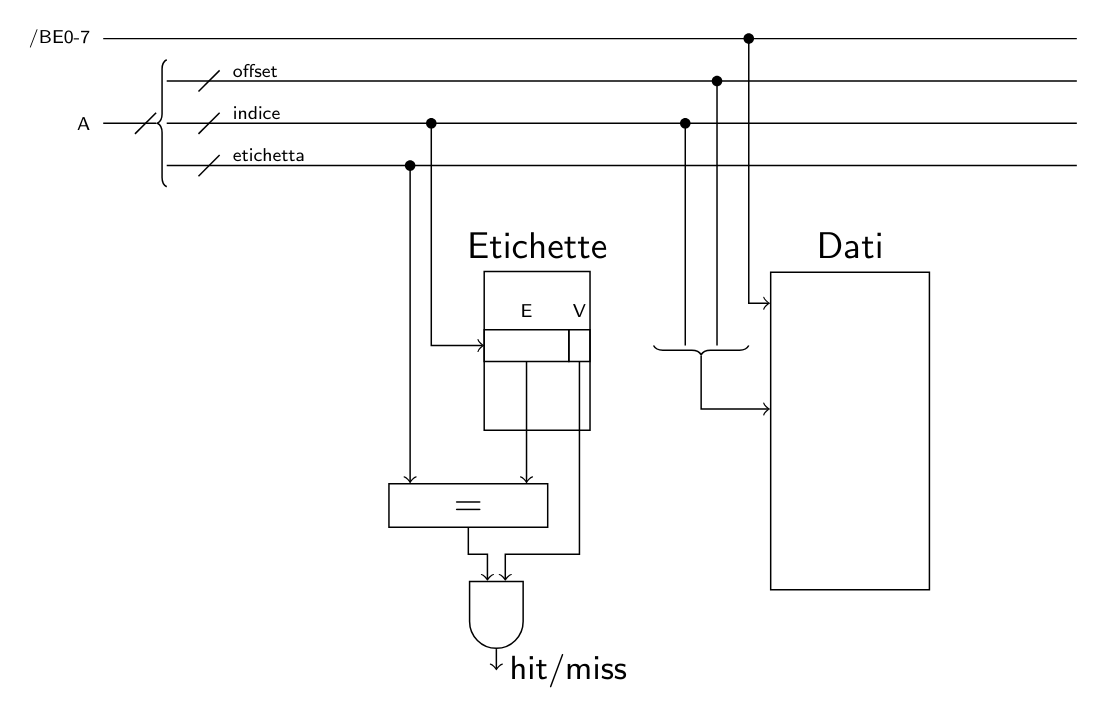
\includegraphics[scale = 0.5]{../figures/cache_diretta.png}
\end{center}
\end{minipage}

\subsubsection{Lettura}
A questo punto, in fase di lettura, nel caso di hit basterà ricavare una linea di offset dai bit meno significativi di A, e leggere dalla memoria cache a tale offset, all'indice indicato dall'etichetta.
Nel caso di miss si dovrà invece svolgere la lettura in memoria RAM, e poi riportare l'informazione nella cacheline di indice giusto della cache aggiornando l'etichetta.

\subsubsection{Scrittura}
Per quanto riguarda le scritture invece, potremo muoverci in due strade: \textbf{write allocate} e \textbf{write no allocate}.

\begin{itemize}
	\item \textbf{Write allocate:}
ci comportiamo in maniera simile alla lettura nel caso di hit.
Nel caso di miss, invece, riportiamo il dato in cache.

A questo punto potremmo pensare di svolgere la scrittura in RAM e in cache contemporaneamente (regola \textit{write-through}), mantenendo entrambe aggiornate.

Una tecnica più intelligente può invece essere quella di aggiornare il solo dato in cache, e rimandare la scrittura in RAM alla rimozione del dato dalla cache (per l'introduzione di un nuovo dato allo stesso indice) (regola \textit{write-back}).
In questo caso dovremo dotarci di un nuovo bit nella memoria delle etichette, il bit \textit{dirty}, che segnalerà il bisogno di ricopiare il dato in cache nella RAM in occasione del suo deallocamento dalla cache.
La difficoltà principale di questo metodo è l'avere un agente che non è la CPU che scrive in RAM, e come vedremo richiede soluzioni tecniche particolari.

\item \textbf{Write no allocate:}
in questo caso ignoriamo le scritture in cache e la sfruttiamo solamente per le letture.

\end{itemize}

\par\smallskip

Notiamo che questa cache soffre di problemi di \textbf{collisione}: infatti ci sarà un numero di regioni con lo stesso indice ed etichetta diversa, pari alla dimensione della RAM fratto la dimensione della cache.

\end{document}


\documentclass[a4paper,11pt]{article}
\usepackage[a4paper, margin=8em]{geometry}

% usa i pacchetti per la scrittura in italiano
\usepackage[french,italian]{babel}
\usepackage[T1]{fontenc}
\usepackage[utf8]{inputenc}
\frenchspacing 

% usa i pacchetti per la formattazione matematica
\usepackage{amsmath, amssymb, amsthm, amsfonts}

% usa altri pacchetti
\usepackage{gensymb}
\usepackage{hyperref}
\usepackage{standalone}

\usepackage{colortbl}

\usepackage{xstring}
\usepackage{karnaugh-map}

% imposta il titolo
\title{Appunti Calcolatori Elettronici}
\author{Luca Seggiani}
\date{2025}

% imposta lo stile
% usa helvetica
\usepackage[scaled]{helvet}
% usa palatino
\usepackage{palatino}
% usa un font monospazio guardabile
\usepackage{lmodern}

\renewcommand{\rmdefault}{ppl}
\renewcommand{\sfdefault}{phv}
\renewcommand{\ttdefault}{lmtt}

% circuiti
\usepackage{circuitikz}
\usetikzlibrary{babel}

% testo cerchiato
\newcommand*\circled[1]{\tikz[baseline=(char.base)]{
            \node[shape=circle,draw,inner sep=2pt] (char) {#1};}}

% disponi il titolo
\makeatletter
\renewcommand{\maketitle} {
	\begin{center} 
		\begin{minipage}[t]{.8\textwidth}
			\textsf{\huge\bfseries \@title} 
		\end{minipage}%
		\begin{minipage}[t]{.2\textwidth}
			\raggedleft \vspace{-1.65em}
			\textsf{\small \@author} \vfill
			\textsf{\small \@date}
		\end{minipage}
		\par
	\end{center}

	\thispagestyle{empty}
	\pagestyle{fancy}
}
\makeatother

% disponi teoremi
\usepackage{tcolorbox}
\newtcolorbox[auto counter, number within=section]{theorem}[2][]{%
	colback=blue!10, 
	colframe=blue!40!black, 
	sharp corners=northwest,
	fonttitle=\sffamily\bfseries, 
	title=Teorema~\thetcbcounter: #2, 
	#1
}

% disponi definizioni
\newtcolorbox[auto counter, number within=section]{definition}[2][]{%
	colback=red!10,
	colframe=red!40!black,
	sharp corners=northwest,
	fonttitle=\sffamily\bfseries,
	title=Definizione~\thetcbcounter: #2,
	#1
}

% disponi codice
\usepackage{listings}
\usepackage[table]{xcolor}

\definecolor{codegreen}{rgb}{0,0.6,0}
\definecolor{codegray}{rgb}{0.5,0.5,0.5}
\definecolor{codepurple}{rgb}{0.58,0,0.82}
\definecolor{backcolour}{rgb}{0.95,0.95,0.92}

\lstdefinestyle{codestyle}{
		backgroundcolor=\color{black!5}, 
		commentstyle=\color{codegreen},
		keywordstyle=\bfseries\color{magenta},
		numberstyle=\sffamily\tiny\color{black!60},
		stringstyle=\color{green!50!black},
		basicstyle=\ttfamily\footnotesize,
		breakatwhitespace=false,         
		breaklines=true,                 
		captionpos=b,                    
		keepspaces=true,                 
		numbers=left,                    
		numbersep=5pt,                  
		showspaces=false,                
		showstringspaces=false,
		showtabs=false,                  
		tabsize=2
}

\lstdefinestyle{shellstyle}{
		backgroundcolor=\color{black!5}, 
		basicstyle=\ttfamily\footnotesize\color{black}, 
		commentstyle=\color{black}, 
		keywordstyle=\color{black},
		numberstyle=\color{black!5},
		stringstyle=\color{black}, 
		showspaces=false,
		showstringspaces=false, 
		showtabs=false, 
		tabsize=2, 
		numbers=none, 
		breaklines=true
}


\lstdefinelanguage{assembler}{ 
  keywords={AAA, AAD, AAM, AAS, ADC, ADCB, ADCW, ADCL, ADD, ADDB, ADDW, ADDL, AND, ANDB, ANDW, ANDL,
        ARPL, BOUND, BSF, BSFL, BSFW, BSR, BSRL, BSRW, BSWAP, BT, BTC, BTCB, BTCW, BTCL, BTR, 
        BTRB, BTRW, BTRL, BTS, BTSB, BTSW, BTSL, CALL, CBW, CDQ, CLC, CLD, CLI, CLTS, CMC, CMP,
        CMPB, CMPW, CMPL, CMPS, CMPSB, CMPSD, CMPSW, CMPXCHG, CMPXCHGB, CMPXCHGW, CMPXCHGL,
        CMPXCHG8B, CPUID, CWDE, DAA, DAS, DEC, DECB, DECW, DECL, DIV, DIVB, DIVW, DIVL, ENTER,
        HLT, IDIV, IDIVB, IDIVW, IDIVL, IMUL, IMULB, IMULW, IMULL, IN, INB, INW, INL, INC, INCB,
        INCW, INCL, INS, INSB, INSD, INSW, INT, INT3, INTO, INVD, INVLPG, IRET, IRETD, JA, JAE,
        JB, JBE, JC, JCXZ, JE, JECXZ, JG, JGE, JL, JLE, JMP, JNA, JNAE, JNB, JNBE, JNC, JNE, JNG,
        JNGE, JNL, JNLE, JNO, JNP, JNS, JNZ, JO, JP, JPE, JPO, JS, JZ, LAHF, LAR, LCALL, LDS,
        LEA, LEAVE, LES, LFS, LGDT, LGS, LIDT, LMSW, LOCK, LODSB, LODSD, LODSW, LOOP, LOOPE,
        LOOPNE, LSL, LSS, LTR, MOV, MOVB, MOVW, MOVL, MOVSB, MOVSD, MOVSW, MOVSX, MOVSXB,
        MOVSXW, MOVSXL, MOVZX, MOVZXB, MOVZXW, MOVZXL, MUL, MULB, MULW, MULL, NEG, NEGB, NEGW,
        NEGL, NOP, NOT, NOTB, NOTW, NOTL, OR, ORB, ORW, ORL, OUT, OUTB, OUTW, OUTL, OUTSB, OUTSD,
        OUTSW, POP, POPL, POPW, POPB, POPA, POPAD, POPF, POPFD, PUSH, PUSHL, PUSHW, PUSHB, PUSHA, 
				PUSHAD, PUSHF, PUSHFD, RCL, RCLB, RCLW, MOVSL, MOVSB, MOVSW, STOSL, STOSB, STOSW, LODSB, LODSW,
				LODSL, INSB, INSW, INSL, OUTSB, OUTSL, OUTSW
        RCLL, RCR, RCRB, RCRW, RCRL, RDMSR, RDPMC, RDTSC, REP, REPE, REPNE, RET, ROL, ROLB, ROLW,
        ROLL, ROR, RORB, RORW, RORL, SAHF, SAL, SALB, SALW, SALL, SAR, SARB, SARW, SARL, SBB,
        SBBB, SBBW, SBBL, SCASB, SCASD, SCASW, SETA, SETAE, SETB, SETBE, SETC, SETE, SETG, SETGE,
        SETL, SETLE, SETNA, SETNAE, SETNB, SETNBE, SETNC, SETNE, SETNG, SETNGE, SETNL, SETNLE,
        SETNO, SETNP, SETNS, SETNZ, SETO, SETP, SETPE, SETPO, SETS, SETZ, SGDT, SHL, SHLB, SHLW,
        SHLL, SHLD, SHR, SHRB, SHRW, SHRL, SHRD, SIDT, SLDT, SMSW, STC, STD, STI, STOSB, STOSD,
        STOSW, STR, SUB, SUBB, SUBW, SUBL, TEST, TESTB, TESTW, TESTL, VERR, VERW, WAIT, WBINVD,
        XADD, XADDB, XADDW, XADDL, XCHG, XCHGB, XCHGW, XCHGL, XLAT, XLATB, XOR, XORB, XORW, XORL},
  keywordstyle=\color{blue}\bfseries,
  ndkeywordstyle=\color{darkgray}\bfseries,
  identifierstyle=\color{black},
  sensitive=false,
  comment=[l]{\#},
  morecomment=[s]{/*}{*/},
  commentstyle=\color{purple}\ttfamily,
  stringstyle=\color{red}\ttfamily,
  morestring=[b]',
  morestring=[b]"
}

\lstset{language=assembler, style=codestyle}

% disponi sezioni
\usepackage{titlesec}

\titleformat{\section}
	{\sffamily\Large\bfseries} 
	{\thesection}{1em}{} 
\titleformat{\subsection}
	{\sffamily\large\bfseries}   
	{\thesubsection}{1em}{} 
\titleformat{\subsubsection}
	{\sffamily\normalsize\bfseries} 
	{\thesubsubsection}{1em}{}

% tikz
\usepackage{tikz}

% float
\usepackage{float}

% grafici
\usepackage{pgfplots}
\pgfplotsset{width=10cm,compat=1.9}

% disponi alberi
\usepackage{forest}

\forestset{
	rectstyle/.style={
		for tree={rectangle,draw,font=\large\sffamily}
	},
	roundstyle/.style={
		for tree={circle,draw,font=\large}
	}
}

% disponi algoritmi
\usepackage{algorithm}
\usepackage{algorithmic}
\makeatletter
\renewcommand{\ALG@name}{Algoritmo}
\makeatother

% disponi numeri di pagina
\usepackage{fancyhdr}
\fancyhf{} 
\fancyfoot[L]{\sffamily{\thepage}}

\makeatletter
\fancyhead[L]{\raisebox{1ex}[0pt][0pt]{\sffamily{\@title \ \@date}}} 
\fancyhead[R]{\raisebox{1ex}[0pt][0pt]{\sffamily{\@author}}}
\makeatother

\begin{document}
% sezione (data)
\section{Lezione del 07-03-25}

% stili pagina
\thispagestyle{empty}
\pagestyle{fancy}

% testo
Riprendiamo il discorso della memoria cache.
Avevamo che questa è montata fra la CPU e lo spazio di memoria.
Più propriamente, questa si trova fra la CPU e il bus.

In questo, può vedere non solo le operazioni sulla memoria, ma anche sullo spazio di I/O.
In questo caso, però, dovrà ovviamente comportarsi sempre in maniera \textit{read-through} e \textit{write-through}, quindi effettivamente disattivarsi e lasciare che il processore interagisca direttamente con l'I/O.

Questo è dovuto al fatto che allo spazio di I/O potrebbero accedere e modificare dati dispositivi esterni alla CPU (le interfacce), operazione che invaliderebbe immediatamente qualsiasi cosa venga scritta in memoriaa cache.

Inoltre, ogni operazione di lettura può comportare di per sé un aggiornamento delle interfacce, che comporterà un aggiornamento della memoria, motivo per cui un operazione di caching sarebbe superflua.

Operazione simile varrà effettuata per la memoria video (che non sta nello spazio di I/O).
Questa facoltà verra realizzata dalla cache attraverso, probabilmente, \textit{maschere} o \textit{tabelle}.

\subsubsection{Cache associative ad insiemi}
Avevamo visto come il difetto principale della cache ad indirizzamento diretta è quello delle \textit{collisioni}.
Presentiamo un metodo, quello delle \textbf{cache associative ad insiemi}, che risolve il problema permettendo di allocare più cacheline allo stesso indirizzo.

Duplichiamo quindi la struttura vista per la cache ad indirizzamento diretto (qui 2 volte), e sruttiamo le uscite hit/miss delle singole memorie delle etichette per pilotare un multiplexer con in ingresso le linee dati delle memorie di cache corrispondenti.

In questo caso a letture allo stesso indice le cache potranno rispondere diversamente (magari la prima in miss e la seconda in hit), e il processore vedrà ritornarsi il dato corretto (in questo caso quello della seconda).

Compito di scegliere quale cache sfruttare nel caso di collisioni è quello del \textbf{controllore} di cache (nella cache ad indirizzamento diretto non c'era scelta). 
La scelta migliore possibile sarebbe quella di scegliere la cacheline al cui i accederà più tardi nel futuro (per mantenere i dati immediatamente utili nella cache).

Chiaramente, visto che non si può prevedere il futuro (o almeno non lo possono fare né la CPU né il controllore di cache), occorre adottare un euristica.
Una di queste euristiche è la politica \textbf{LRU} (\textit{Least Recently Used}), dove si sceglie la cacheline al quale non si accede da più tempo.

Per realizzare tale politica si sfrutta una memoria, che chiamiamo $R$.
Con solo due vie, basterà memorizzare su $R$ l'ultima via usata, e quella su cui scriviere sarà immediatamente l'altra.

Con più di due vie sarebbe necessario mantenere l'ordine degli accessi, cio per $n$ vie ricordare informazione necessaria a controllare $n!$ diverse possibilità.
Nella pratica, però, conviene usare politiche approssimate.

\subsubsection{Pseudo-LRU dell'80486}
Vediamo una di queste politiche approssimate, che gestiva 4 vie attraverso 3 bit $b_00$, $b_1$ e $b_2$.
Si usava un albero binario per la selezione di una delle vie, disposto come:
\begin{center}
	\begin{forest}
		[$b_0$, roundstyle
			[$b_1$
				[A, rectstyle]
				[B, rectstyle]
				]
			[$b_2$
				[C, rectstyle]
				[D, rectstyle]
			]
		]	
	\end{forest}
\end{center}
dove i valori 1 sono i rami a destra, e viceversa i valori 0 sono i rami a sinistra.

In fase di rimpiazzamento, si sceglie la via seguendo l'albero.
In fase di accesso, si modificano i $b_i$ in modo da portare la via a cui si è fasso accesso in fondo all'ordinamento che si ottiene visitando l'albero.
L'errore può essere dato dal fatto che la via che si trova nello stesso gruppo della via a cui si è fatto accesso potrebbe trovarsi ad un indice più alto del necessario, visto che si abbassa cumulativamente l'intero gruppo aggiornando $b_0$.

\par\smallskip

Per cache più grandi si sfruttano sempre algoritmi ad albero di questo tipo, magari tagliando i rami più bassi per lasciare spazio a scelte completamente casuali.

Notiamo poi che le memorie cache di questo tipo incontrano sempre difficoltà quando si fanno accessi ciclici ad indici che si ripetono con un modulo con il numero di vie diverso da zero: ad esempio se si leggono ciclicamente 5 indirizzi che corrispondono allo stesso indice, la cache non riuscirà mai a mantenere tutti e 5 in una delle cacheline delle vie, e quindi ogni accesso comporterà un miss.

\subsubsection{Livelli di cache}
Nei processori moderni si hanno solitamente più livelli di cache (3 o 4), che crescono in dimensioni e associatività più si vanno a disporre "lontano" dal processore e "vicini" alla RAM.
Le cache di livello più basso saranno quindi più veloci ma più piccole, mentre le cache di livelo alto saranno più lente ma più grandi.

Il controllore di cache provvederà a gestire i livelli di cache, effettuando gli accessi controllando a partire dal livello più basso (più veloce) per arrivare al livello più basso, fino alla RAM.

\subsection{Interruzioni}
La limitazione principale del processore studiato finora è che il flusso di controllo è completamente determinato dal programma in esecuzione.
Attraverso il meccanismo dell'interruzione, il sistema definisce $e_1, ..., e_n$ \textbf{eventi}, e il programmatore $r_1, ..., r_n$ \textbf{routine} per la gestione di tali eventi.
Da qui in poi il processore continua ad eseguire il suo normale flusso di controllo, ma monitorando in qualche modo lo stato di questi eventi.
Nel caso uno degli eventi $e_i$ effettivamente si verifichi, la CPU provvederà a sospendere il flusso di controllo attuale e ad eseguire la routine $r_i$.

Un esempio classico dell'utilità di un meccanismo di questo tipo è dato dalle fasi di stampa che avevamo definito per dispositivi come le stampanti: attraverso l'approcio visto finora dovremmo controllare periodicamente un certo registro di stato per verificare la possibilità di scrivere un nuovo dato in un certo registro di buffer.
Questo occupa la CPU con operazioni inutili, che potrebbe saltare se fosse la stampante stessa ad avvertirla di quando è pronta a ricevere un nuovo dato.

L'idea di base è quella di avere una nuova operazione da svolgere in fase di esecuzione di un instruzione da parte della CPU, dopo l'esecuzione dell'istruzione stessa.
Ad esempio, potremmo riportarci un bit di valdiità, \lstinline|READY|, da parte della stampante, e controllarlo ad ogni istruzione per la chiamata di una routine di stampa.
La chiamata sarà semplicemente un aggiornamento condizionato a RIP, con scrittura del contenuto attuale di RIP in pila (che è compatibile con le regole di chiamata dei sottoprogrammi a cui siamo abituati).

Un problema di questo approccio potrebbe essere che, se il bit che segnala l'evento non si aggiorna immediatamente, la CPU andrà in un ciclo continuo di arresto dell'esecuzione e inizio di una routine.
Una soluzione potrebbe essere dotare della CPU di una \textit{rete di accettazione} della richiesta: il bit di segnalazione dell'evento va in un generatore di impulsi che setta un SR flip-flop. 
A questo punto la CPU risponde (livello hardware, nella nuova fase di esecuzione appena descritta) con un segnale di reset nel momento in cui riesce a rilevare l'evento e spostarsi nella routine. 

In verità la situazione è più complicata: ad esempio potremmo voler ignorare nuovi eventi quando stiamo già cercando di soddisfarne uno.
Per questo i processori x86 prevedono un apposito flag, il flag \textbf{IF} (\textit{Interruption Flag}), che determina se le nuove interruzioni dovranno essere soddisfatte o meno.
Il processore può essere quindi configurato per attivare automaticamente il flag IF in fase di risposta ad una richiesta di interruzione.
Per effettuare il corretto ritorno, si usa la funzione \lstinline|IRETQ|, che ripristina, oltre ad altre cose, lo stato dei flag (che era stato salvato in pila).



\end{document}


\documentclass[a4paper,11pt]{article}
\usepackage[a4paper, margin=8em]{geometry}

% usa i pacchetti per la scrittura in italiano
\usepackage[french,italian]{babel}
\usepackage[T1]{fontenc}
\usepackage[utf8]{inputenc}
\frenchspacing 

% usa i pacchetti per la formattazione matematica
\usepackage{amsmath, amssymb, amsthm, amsfonts}

% usa altri pacchetti
\usepackage{gensymb}
\usepackage{hyperref}
\usepackage{standalone}

\usepackage{colortbl}

\usepackage{xstring}
\usepackage{karnaugh-map}

% imposta il titolo
\title{Appunti Calcolatori Elettronici}
\author{Luca Seggiani}
\date{2025}

% imposta lo stile
% usa helvetica
\usepackage[scaled]{helvet}
% usa palatino
\usepackage{palatino}
% usa un font monospazio guardabile
\usepackage{lmodern}

\renewcommand{\rmdefault}{ppl}
\renewcommand{\sfdefault}{phv}
\renewcommand{\ttdefault}{lmtt}

% circuiti
\usepackage{circuitikz}
\usetikzlibrary{babel}

% testo cerchiato
\newcommand*\circled[1]{\tikz[baseline=(char.base)]{
            \node[shape=circle,draw,inner sep=2pt] (char) {#1};}}

% disponi il titolo
\makeatletter
\renewcommand{\maketitle} {
	\begin{center} 
		\begin{minipage}[t]{.8\textwidth}
			\textsf{\huge\bfseries \@title} 
		\end{minipage}%
		\begin{minipage}[t]{.2\textwidth}
			\raggedleft \vspace{-1.65em}
			\textsf{\small \@author} \vfill
			\textsf{\small \@date}
		\end{minipage}
		\par
	\end{center}

	\thispagestyle{empty}
	\pagestyle{fancy}
}
\makeatother

% disponi teoremi
\usepackage{tcolorbox}
\newtcolorbox[auto counter, number within=section]{theorem}[2][]{%
	colback=blue!10, 
	colframe=blue!40!black, 
	sharp corners=northwest,
	fonttitle=\sffamily\bfseries, 
	title=Teorema~\thetcbcounter: #2, 
	#1
}

% disponi definizioni
\newtcolorbox[auto counter, number within=section]{definition}[2][]{%
	colback=red!10,
	colframe=red!40!black,
	sharp corners=northwest,
	fonttitle=\sffamily\bfseries,
	title=Definizione~\thetcbcounter: #2,
	#1
}

% disponi codice
\usepackage{listings}
\usepackage[table]{xcolor}

\definecolor{codegreen}{rgb}{0,0.6,0}
\definecolor{codegray}{rgb}{0.5,0.5,0.5}
\definecolor{codepurple}{rgb}{0.58,0,0.82}
\definecolor{backcolour}{rgb}{0.95,0.95,0.92}

\lstdefinestyle{codestyle}{
		backgroundcolor=\color{black!5}, 
		commentstyle=\color{codegreen},
		keywordstyle=\bfseries\color{magenta},
		numberstyle=\sffamily\tiny\color{black!60},
		stringstyle=\color{green!50!black},
		basicstyle=\ttfamily\footnotesize,
		breakatwhitespace=false,         
		breaklines=true,                 
		captionpos=b,                    
		keepspaces=true,                 
		numbers=left,                    
		numbersep=5pt,                  
		showspaces=false,                
		showstringspaces=false,
		showtabs=false,                  
		tabsize=2
}

\lstdefinestyle{shellstyle}{
		backgroundcolor=\color{black!5}, 
		basicstyle=\ttfamily\footnotesize\color{black}, 
		commentstyle=\color{black}, 
		keywordstyle=\color{black},
		numberstyle=\color{black!5},
		stringstyle=\color{black}, 
		showspaces=false,
		showstringspaces=false, 
		showtabs=false, 
		tabsize=2, 
		numbers=none, 
		breaklines=true
}


\lstdefinelanguage{assembler}{ 
  keywords={AAA, AAD, AAM, AAS, ADC, ADCB, ADCW, ADCL, ADD, ADDB, ADDW, ADDL, AND, ANDB, ANDW, ANDL,
        ARPL, BOUND, BSF, BSFL, BSFW, BSR, BSRL, BSRW, BSWAP, BT, BTC, BTCB, BTCW, BTCL, BTR, 
        BTRB, BTRW, BTRL, BTS, BTSB, BTSW, BTSL, CALL, CBW, CDQ, CLC, CLD, CLI, CLTS, CMC, CMP,
        CMPB, CMPW, CMPL, CMPS, CMPSB, CMPSD, CMPSW, CMPXCHG, CMPXCHGB, CMPXCHGW, CMPXCHGL,
        CMPXCHG8B, CPUID, CWDE, DAA, DAS, DEC, DECB, DECW, DECL, DIV, DIVB, DIVW, DIVL, ENTER,
        HLT, IDIV, IDIVB, IDIVW, IDIVL, IMUL, IMULB, IMULW, IMULL, IN, INB, INW, INL, INC, INCB,
        INCW, INCL, INS, INSB, INSD, INSW, INT, INT3, INTO, INVD, INVLPG, IRET, IRETD, JA, JAE,
        JB, JBE, JC, JCXZ, JE, JECXZ, JG, JGE, JL, JLE, JMP, JNA, JNAE, JNB, JNBE, JNC, JNE, JNG,
        JNGE, JNL, JNLE, JNO, JNP, JNS, JNZ, JO, JP, JPE, JPO, JS, JZ, LAHF, LAR, LCALL, LDS,
        LEA, LEAVE, LES, LFS, LGDT, LGS, LIDT, LMSW, LOCK, LODSB, LODSD, LODSW, LOOP, LOOPE,
        LOOPNE, LSL, LSS, LTR, MOV, MOVB, MOVW, MOVL, MOVSB, MOVSD, MOVSW, MOVSX, MOVSXB,
        MOVSXW, MOVSXL, MOVZX, MOVZXB, MOVZXW, MOVZXL, MUL, MULB, MULW, MULL, NEG, NEGB, NEGW,
        NEGL, NOP, NOT, NOTB, NOTW, NOTL, OR, ORB, ORW, ORL, OUT, OUTB, OUTW, OUTL, OUTSB, OUTSD,
        OUTSW, POP, POPL, POPW, POPB, POPA, POPAD, POPF, POPFD, PUSH, PUSHL, PUSHW, PUSHB, PUSHA, 
				PUSHAD, PUSHF, PUSHFD, RCL, RCLB, RCLW, MOVSL, MOVSB, MOVSW, STOSL, STOSB, STOSW, LODSB, LODSW,
				LODSL, INSB, INSW, INSL, OUTSB, OUTSL, OUTSW
        RCLL, RCR, RCRB, RCRW, RCRL, RDMSR, RDPMC, RDTSC, REP, REPE, REPNE, RET, ROL, ROLB, ROLW,
        ROLL, ROR, RORB, RORW, RORL, SAHF, SAL, SALB, SALW, SALL, SAR, SARB, SARW, SARL, SBB,
        SBBB, SBBW, SBBL, SCASB, SCASD, SCASW, SETA, SETAE, SETB, SETBE, SETC, SETE, SETG, SETGE,
        SETL, SETLE, SETNA, SETNAE, SETNB, SETNBE, SETNC, SETNE, SETNG, SETNGE, SETNL, SETNLE,
        SETNO, SETNP, SETNS, SETNZ, SETO, SETP, SETPE, SETPO, SETS, SETZ, SGDT, SHL, SHLB, SHLW,
        SHLL, SHLD, SHR, SHRB, SHRW, SHRL, SHRD, SIDT, SLDT, SMSW, STC, STD, STI, STOSB, STOSD,
        STOSW, STR, SUB, SUBB, SUBW, SUBL, TEST, TESTB, TESTW, TESTL, VERR, VERW, WAIT, WBINVD,
        XADD, XADDB, XADDW, XADDL, XCHG, XCHGB, XCHGW, XCHGL, XLAT, XLATB, XOR, XORB, XORW, XORL},
  keywordstyle=\color{blue}\bfseries,
  ndkeywordstyle=\color{darkgray}\bfseries,
  identifierstyle=\color{black},
  sensitive=false,
  comment=[l]{\#},
  morecomment=[s]{/*}{*/},
  commentstyle=\color{purple}\ttfamily,
  stringstyle=\color{red}\ttfamily,
  morestring=[b]',
  morestring=[b]"
}

\lstset{language=assembler, style=codestyle}

% disponi sezioni
\usepackage{titlesec}

\titleformat{\section}
	{\sffamily\Large\bfseries} 
	{\thesection}{1em}{} 
\titleformat{\subsection}
	{\sffamily\large\bfseries}   
	{\thesubsection}{1em}{} 
\titleformat{\subsubsection}
	{\sffamily\normalsize\bfseries} 
	{\thesubsubsection}{1em}{}

% tikz
\usepackage{tikz}

% float
\usepackage{float}

% grafici
\usepackage{pgfplots}
\pgfplotsset{width=10cm,compat=1.9}

% disponi alberi
\usepackage{forest}

\forestset{
	rectstyle/.style={
		for tree={rectangle,draw,font=\large\sffamily}
	},
	roundstyle/.style={
		for tree={circle,draw,font=\large}
	}
}

% disponi algoritmi
\usepackage{algorithm}
\usepackage{algorithmic}
\makeatletter
\renewcommand{\ALG@name}{Algoritmo}
\makeatother

% disponi numeri di pagina
\usepackage{fancyhdr}
\fancyhf{} 
\fancyfoot[L]{\sffamily{\thepage}}

\makeatletter
\fancyhead[L]{\raisebox{1ex}[0pt][0pt]{\sffamily{\@title \ \@date}}} 
\fancyhead[R]{\raisebox{1ex}[0pt][0pt]{\sffamily{\@author}}}
\makeatother

\begin{document}
% sezione (data)
\section{Lezione del 10-03-25}

% stili pagina
\thispagestyle{empty}
\pagestyle{fancy}

% testo
Torniamo sull'argomento delle interruzioni, specificando il modo in cui dobbiamo definire dei \textit{gestori} per ogni interruzione.

Il calcolatore visto finora dispone di 4 interfacce: \begin{itemize}
	\item L'interfaccia \textit{tastiera}, letta finora in controllo di programma, valutando la validità di un bit FI sul registro di stato;
	\item L'interfaccia \textit{timer}, dotata di 3 singoli timer, di cui abbiamo detto il primo viene usato per generare interruzioni, il secondo non è più usato, e il terzo e connesso al \textit{beeper speaker};
	\item L'interfaccia a blocchi per \textit{hard disk}, che accede ad un drive pilotando in base al suo stato un registro di stato (per noi era utile implementare la funzione di attesa del drive a controllo programma \lstinline|wait_for_br()|).
\end{itemize} 

Ignoriamo, per adesso, il video.
Ognuna di queste interfacce può trarre beneficio dalla presenza di interruzioni:
\begin{itemize}
	\item La tastiera potrebbe \textit{avvertirci} dei nuovi tasti premuti, anziché costringerci a controllare;
	\item Il timer ci deve avvisare, al termine del conteggio del timer 0, attraverso un interruzione;
	\item L'hard disk, come la tastiera, ci può avvisare con un interruzione quando è pronto ad una nuova scrittura.
\end{itemize}

Questo comportamento, delle cosiddette \textbf{interruzioni esterne}, è definito nella macchina studiata dal \textbf{controllore delle interruzioni}, che è l'Intel \textbf{APIC} (\textit{Advanced Progammable Interruption Controller}).
Questo scansiona periodicamente tutte le linee di richiesta d'interruzione (le \textbf{IRQ}) ottenute dalle varie interfacce, e invia le interruzioni corrispondenti, una per volta, alla CPU. 

Avevamo già reputato necessario specificare un \textbf{tipo di interruzione}, su 8 bit (per 256 tipi) per ogni interruzione lanciata.
L'APIC, allora, fornirà semplicemente la possibilità di assegnare un tipo di interruzione diverso ad ogni piedino di ingresso dall interfacce, in modo che si possa assegnare ad ogni interruzione la routine di gestione più adatta.
In questo, la configurazione dell'APIC si svolge come la configurazione di una qualsiasi periferica attraverso un'apposita interfaccia.

La comunicazione fra CPU e APIC in fase di interruzione viene effettuata attraverso un \textit{handshake} su due linee, \textbf{INTR} (\textit{Interrupt Request}) e \textbf{INTA} (\textit{Interrupt Acknowledge}), che comporta anche una lettura da parte della CPU di quanto l'APIC metterà sul bus (cioè il tipo di interruzione).

A questo punto, le routine vere e proprie verrano definite nell'\textbf{IDT}, (\textit{Interrupt Descriptor Table}), contenente in sequenza gli indirizzi delle prime istruzioni di ogni routine per ogni tipo di interruzione, e specificata a partire da un certo indirizzo indicato nel registro \textbf{IDTR}.

Come abbiamo visto, la reazione o meno della CPU ad una interuzione è data dall'attivazione del flag IF.
Nel caso si passi effettivamente ad eseguire l'interruzione, ricordiamo che sia l'IP che lo stato dei flags verrà salvato in pila, e ripristinato a fine routine attraverso l'istruzione \lstinline|IRET|.

\subsubsection{Rilevamento di interruzioni da parte dell'APIC}
Potremmo chiederci come fa il controllore APIC a capire quando un'interfaccia sta richiedendo una nuova richiesta.

Un primo approccio potrebbe essere di non rileggere il piedino di ingresso di quell'interfaccia, all'ottenimento e successivo invio alla CPU di un interruzione, fino alla segnalazione, sempre da parte della CPU, di avvenuta gestione dell'interruzione.
Questo può essere effettuato dotando l'APIC di un opportuno registro (\textbf{EOI}, \textit{End Of Interrupt}), che la CPU andrà a modificare conclusa la gestione dell'interruzione.

Un approccio più sicuro può essere ottenuto dotando il controllore delle interruzioni di due registri, entrambi su 256 bit (un bit per ogni tipo di interruzione):
\begin{itemize}
	\item \textbf{IRR} (\textit{Interrupt Request Register}): indica con bit alti quali interruzioni sono state inviate dalle interfacce attualmente;
	\item \textbf{ISR} (\textit{Interrupt Service Register}): indica con bit alti a quali interruzioni sta rispondendo il processore attualmente. In un processore single-threaded come quello che studiamo al più uno solo dei suoi bit sarà alto in un dato momento (escluso il caso della \textit{gestione annidata}).
\end{itemize}

Si avrà quindi la seguente organizzazione:
\begin{table}[h!]
	\center 
	\begin{tabular} { c | c  }
		\textbf{IRR}, \textit{Interrupt Request Register} & 256 bit \\
		\textbf{ISR}, \textit{Interrupt Service Register} & 256 bit
	\end{tabular}
\end{table}

Un interruzione generata lato hardware si tradurrà nell'innalzamento (se non era già alto) di un bit nell'IRR, e l'inizio (o schedulazione dell'inizio) di un handshake con la CPU.
Al termine dell'handshake (quindi all'abbassamento di INTA successivo ad un suo innalzamento per acknowledge) il bit dell'interruzione corrente passa dall'IRR all'ISR.
Infine, la transizione dal bit presente nell'ISR all'interruzione gestita (bit nuovamente basso) si ha sempre con il segnale EOI da parte della CPU (con successivo inizio, se necessario, di un nuovo ciclo di handshake per una nuova richiesta di interruzione).

\subsubsection{Priorità delle interruzioni e gestione annidata}
Ci rendiamo quindi conto che alcune richieste sono più importanti di altre: ad esempio, la pressione di un tasto su tastiera può essere ignorata, se ad esempio nel frattempo arriva una richiesta di interruzione da parte di un timer.
La pressione del tasto non si ripeterà infatti in tempo utile, mentre il timer potrebbe inviarci nuove richieste mentre ancora non siamo pronti a riceverle, e continuerà a farlo a scadenze regolari (potremmo finire per gestire solo un sottoinsieme delle richieste che ci vengono effettivamente inviate).

Possiamo quindi chiederci come l'APIC si comporta in caso di più richieste concorrenti.
Un idea potrebbe essere di assegnare una priorità ad ogni richiesta, e rispondere prima alle richieste di priorità più alta.
Questa priorità può essere implementata chiamando i 4 bit più significativi del tipo dell'interruzione \textbf{classe di precedenza} dell'interruzione: a classi di precedenza maggiore abbiamo gestione prioritaria delle richieste di interruzione.
Il trasferimento da IRR a ISR avverrà quindi prima per richieste di classe di precedenza più alta, e poi per quelle di classe di precedenza \textit{uguale} o più bassa, con la possibilità per le prime di \textit{interrompere} i gestori di interruzione delle ultime.

La precedenza delle interruzioni è quindi necessaria all'implementazione corretta della \textbf{gestione annidata} delle interruzioni, dove un interruzione di precedenza più altra può interrompere (a patto che IF sia alto) un gestore di interruzione in esecuzione. 
Questo è il caso a cui accennavamo prima, dove più bit di ISR possono essere alti contemporaneamente (a patto che si dispongano nel tempo, da destra verso sinistra, cioè da minore priorità a maggiore priorità), e che si risolvano da sinistra verso destra (cioè da maggiore priorità a minore priorità).

\end{document}


\documentclass[a4paper,11pt]{article}
\usepackage[a4paper, margin=8em]{geometry}

% usa i pacchetti per la scrittura in italiano
\usepackage[french,italian]{babel}
\usepackage[T1]{fontenc}
\usepackage[utf8]{inputenc}
\frenchspacing 

% usa i pacchetti per la formattazione matematica
\usepackage{amsmath, amssymb, amsthm, amsfonts}

% usa altri pacchetti
\usepackage{gensymb}
\usepackage{hyperref}
\usepackage{standalone}

\usepackage{colortbl}

\usepackage{xstring}
\usepackage{karnaugh-map}

% imposta il titolo
\title{Appunti Calcolatori Elettronici}
\author{Luca Seggiani}
\date{2025}

% imposta lo stile
% usa helvetica
\usepackage[scaled]{helvet}
% usa palatino
\usepackage{palatino}
% usa un font monospazio guardabile
\usepackage{lmodern}

\renewcommand{\rmdefault}{ppl}
\renewcommand{\sfdefault}{phv}
\renewcommand{\ttdefault}{lmtt}

% circuiti
\usepackage{circuitikz}
\usetikzlibrary{babel}

% testo cerchiato
\newcommand*\circled[1]{\tikz[baseline=(char.base)]{
\node[shape=circle,draw,inner sep=2pt] (char) {#1};}}

% disponi il titolo
\makeatletter
\renewcommand{\maketitle} {
	\begin{center} 
		\begin{minipage}[t]{.8\textwidth}
			\textsf{\huge\bfseries \@title} 
		\end{minipage}%
		\begin{minipage}[t]{.2\textwidth}
			\raggedleft \vspace{-1.65em}
			\textsf{\small \@author} \vfill
			\textsf{\small \@date}
		\end{minipage}
		\par
	\end{center}

	\thispagestyle{empty}
	\pagestyle{fancy}
}
\makeatother

% disponi teoremi
\usepackage{tcolorbox}
\newtcolorbox[auto counter, number within=section]{theorem}[2][]{%
	colback=blue!10, 
	colframe=blue!40!black, 
	sharp corners=northwest,
	fonttitle=\sffamily\bfseries, 
	title=Teorema~\thetcbcounter: #2, 
	#1
}

% disponi definizioni
\newtcolorbox[auto counter, number within=section]{definition}[2][]{%
	colback=red!10,
	colframe=red!40!black,
	sharp corners=northwest,
	fonttitle=\sffamily\bfseries,
	title=Definizione~\thetcbcounter: #2,
	#1
}

% disponi codice
\usepackage{listings}
\usepackage[table]{xcolor}

\definecolor{codegreen}{rgb}{0,0.6,0}
\definecolor{codegray}{rgb}{0.5,0.5,0.5}
\definecolor{codepurple}{rgb}{0.58,0,0.82}
\definecolor{backcolour}{rgb}{0.95,0.95,0.92}

\lstdefinestyle{codestyle}{
	backgroundcolor=\color{black!5}, 
	commentstyle=\color{codegreen},
	keywordstyle=\bfseries\color{magenta},
	numberstyle=\sffamily\tiny\color{black!60},
	stringstyle=\color{green!50!black},
	basicstyle=\ttfamily\footnotesize,
	breakatwhitespace=false,         
	breaklines=true,                 
	captionpos=b,                    
	keepspaces=true,                 
	numbers=left,                    
	numbersep=5pt,                  
	showspaces=false,                
	showstringspaces=false,
	showtabs=false,                  
	tabsize=2
}

\lstdefinestyle{shellstyle}{
	backgroundcolor=\color{black!5}, 
	basicstyle=\ttfamily\footnotesize\color{black}, 
	commentstyle=\color{black}, 
	keywordstyle=\color{black},
	numberstyle=\color{black!5},
	stringstyle=\color{black}, 
	showspaces=false,
	showstringspaces=false, 
	showtabs=false, 
	tabsize=2, 
	numbers=none, 
	breaklines=true
}


\lstdefinelanguage{assembler}{ 
	keywords={AAA, AAD, AAM, AAS, ADC, ADCB, ADCW, ADCL, ADD, ADDB, ADDW, ADDL, AND, ANDB, ANDW, ANDL,
		ARPL, BOUND, BSF, BSFL, BSFW, BSR, BSRL, BSRW, BSWAP, BT, BTC, BTCB, BTCW, BTCL, BTR, 
		BTRB, BTRW, BTRL, BTS, BTSB, BTSW, BTSL, CALL, CBW, CDQ, CLC, CLD, CLI, CLTS, CMC, CMP,
		CMPB, CMPW, CMPL, CMPS, CMPSB, CMPSD, CMPSW, CMPXCHG, CMPXCHGB, CMPXCHGW, CMPXCHGL,
		CMPXCHG8B, CPUID, CWDE, DAA, DAS, DEC, DECB, DECW, DECL, DIV, DIVB, DIVW, DIVL, ENTER,
		HLT, IDIV, IDIVB, IDIVW, IDIVL, IMUL, IMULB, IMULW, IMULL, IN, INB, INW, INL, INC, INCB,
		INCW, INCL, INS, INSB, INSD, INSW, INT, INT3, INTO, INVD, INVLPG, IRET, IRETD, JA, JAE,
		JB, JBE, JC, JCXZ, JE, JECXZ, JG, JGE, JL, JLE, JMP, JNA, JNAE, JNB, JNBE, JNC, JNE, JNG,
		JNGE, JNL, JNLE, JNO, JNP, JNS, JNZ, JO, JP, JPE, JPO, JS, JZ, LAHF, LAR, LCALL, LDS,
		LEA, LEAVE, LES, LFS, LGDT, LGS, LIDT, LMSW, LOCK, LODSB, LODSD, LODSW, LOOP, LOOPE,
		LOOPNE, LSL, LSS, LTR, MOV, MOVB, MOVW, MOVL, MOVSB, MOVSD, MOVSW, MOVSX, MOVSXB,
		MOVSXW, MOVSXL, MOVZX, MOVZXB, MOVZXW, MOVZXL, MUL, MULB, MULW, MULL, NEG, NEGB, NEGW,
		NEGL, NOP, NOT, NOTB, NOTW, NOTL, OR, ORB, ORW, ORL, OUT, OUTB, OUTW, OUTL, OUTSB, OUTSD,
		OUTSW, POP, POPL, POPW, POPB, POPA, POPAD, POPF, POPFD, PUSH, PUSHL, PUSHW, PUSHB, PUSHA, 
		PUSHAD, PUSHF, PUSHFD, RCL, RCLB, RCLW, MOVSL, MOVSB, MOVSW, STOSL, STOSB, STOSW, LODSB, LODSW,
		LODSL, INSB, INSW, INSL, OUTSB, OUTSL, OUTSW
		RCLL, RCR, RCRB, RCRW, RCRL, RDMSR, RDPMC, RDTSC, REP, REPE, REPNE, RET, ROL, ROLB, ROLW,
		ROLL, ROR, RORB, RORW, RORL, SAHF, SAL, SALB, SALW, SALL, SAR, SARB, SARW, SARL, SBB,
		SBBB, SBBW, SBBL, SCASB, SCASD, SCASW, SETA, SETAE, SETB, SETBE, SETC, SETE, SETG, SETGE,
		SETL, SETLE, SETNA, SETNAE, SETNB, SETNBE, SETNC, SETNE, SETNG, SETNGE, SETNL, SETNLE,
		SETNO, SETNP, SETNS, SETNZ, SETO, SETP, SETPE, SETPO, SETS, SETZ, SGDT, SHL, SHLB, SHLW,
		SHLL, SHLD, SHR, SHRB, SHRW, SHRL, SHRD, SIDT, SLDT, SMSW, STC, STD, STI, STOSB, STOSD,
		STOSW, STR, SUB, SUBB, SUBW, SUBL, TEST, TESTB, TESTW, TESTL, VERR, VERW, WAIT, WBINVD,
	XADD, XADDB, XADDW, XADDL, XCHG, XCHGB, XCHGW, XCHGL, XLAT, XLATB, XOR, XORB, XORW, XORL},
	keywordstyle=\color{blue}\bfseries,
	ndkeywordstyle=\color{darkgray}\bfseries,
	identifierstyle=\color{black},
	sensitive=false,
	comment=[l]{\#},
	morecomment=[s]{/*}{*/},
	commentstyle=\color{purple}\ttfamily,
	stringstyle=\color{red}\ttfamily,
	morestring=[b]',
	morestring=[b]"
}

\lstset{language=assembler, style=codestyle}

% disponi sezioni
\usepackage{titlesec}

\titleformat{\section}
{\sffamily\Large\bfseries} 
{\thesection}{1em}{} 
\titleformat{\subsection}
{\sffamily\large\bfseries}   
{\thesubsection}{1em}{} 
\titleformat{\subsubsection}
{\sffamily\normalsize\bfseries} 
{\thesubsubsection}{1em}{}

% tikz
\usepackage{tikz}

% float
\usepackage{float}

% grafici
\usepackage{pgfplots}
\pgfplotsset{width=10cm,compat=1.9}

% disponi alberi
\usepackage{forest}

\forestset{
	rectstyle/.style={
		for tree={rectangle,draw,font=\large\sffamily}
	},
	roundstyle/.style={
		for tree={circle,draw,font=\large}
	}
}

% disponi algoritmi
\usepackage{algorithm}
\usepackage{algorithmic}
\makeatletter
\renewcommand{\ALG@name}{Algoritmo}
\makeatother

% disponi numeri di pagina
\usepackage{fancyhdr}
\fancyhf{} 
\fancyfoot[L]{\sffamily{\thepage}}

\makeatletter
\fancyhead[L]{\raisebox{1ex}[0pt][0pt]{\sffamily{\@title \ \@date}}} 
\fancyhead[R]{\raisebox{1ex}[0pt][0pt]{\sffamily{\@author}}}
\makeatother

\begin{document}
% sezione (data)
\section{Lezione del 11-03-25}

% stili pagina
\thispagestyle{empty}
\pagestyle{fancy}

% testo
Riprendiamo la trattazione dell controllore di interruzini APIC.

\subsubsection{Interruzione di livello o di fronte}
Vediamo un dettaglio sul comportamento dell'APIC: questo può rilevare, in base alla sua configurazione, i \textbf{livelli} o i \textbf{fronti} delle variabili in ingresso.

Questo può avere delle implicazioni diverse a seconda dell'interfaccia.
Ad esempio, avevamo detto che il timer in modalità 2 genera un onda quadra.
Se si usa una routine lanciata dal timer a interruzione di programma, e si configura l'APIC per rilevare il livello, potrebbe essere che a routine concluse il livello del timer è sempre alto, e quindi l'interruzione viene lanciata nuovamente.

Questo è chiaramente diverso dal comportamento desiderato, ed è quindi opportuno configurare l'APIC per rilevare i soli fronti di salita.

\par\medskip

Abbiamo quindi notato praticamente tutte le caratteristiche che ci interessavano dell'APIC, e possiamo procedere ad implementare un esempio di gestione di un interfaccia a controllo di interruzione.
Vediamo ad esempio il seguente programma, che gestisce la tastiera a controllo di interruzione, di cui la parte C++:
\lstset{style=codestyle, language=C++}
\lstinputlisting{../code/interrupts/hw_basic/main.cpp}
e la parte assembly:
\lstset{style=codestyle, language=assembler}
\lstinputlisting{../code/interrupts/hw_basic/main.s}

Il meccanismo di chiamata dell'interruzione (macro per il salvataggio/caricamento registri, istruzione \lstinline|iretq|, ecc...) è identico all'esempio precedente.
Una novità è la presenza della funzione \lstinline|send_EOI()| nel gestore di interruzione, che invia il segnale di End Of Interrupt all'APIC e gli fa capire, assieme alla lettura che facciamo sulla tastiera (con \lstinline|kbd::get_code()|) che l'interruzione è stata effettivamente gestita.
Inoltre, la parte di configurazione dell'interruzione è più complessa.
Bisogna infatti:
\begin{itemize}
	\item Attivare le interruzioni da tastiera con \lstinline|kbd::enable_intr()|;
	\item Impostare l'APIC per inviare tali interruzini al tipo interruzione \lstinline|0x20|, configurandolo per riconoscere fronti, e disattivando la maschera (rispettivamente \lstinline|set_TRGM()| e \lstinline|set_MIRQ|);
	\item Infine, inizializzare il gate corrispondente al tipo interruzione \lstinline|0x20| come avevamo già visto.
\end{itemize}

Abbiamo quindi realizzato pienamente quanto ci eravamo posti di fare quando abbiamo iniziato a parlare di interruzione: la CPU è lasciata libera (nell'esempio specifico, esegue un loop infinito), e viene \textit{interrotta} dalla periferica tastiera quando questa ha un nuovo dato disponibile.
Vediamo che in verità esiste un altra casistica di applicazione delle interruzioni che non abbiamo trattato, cioè quella delle \textit{eccezioni}.

\subsection{Eccezioni}
Ci rimangono da vedere le \textbf{eccezioni}.
Queste sono particolari errori logici che il processore potrebbe incontrare nel corso dell'esecuzione, come ad esempio la divisione per 0, il tentativo di eseguire un istruzione non riconosciuta, ecc...

Una differenza fra le interruzioni esterne e le eccezioni è che le eccezioni possono essere sollevate \textit{durante} la lettura e esecuzione di un istruzione, quindi ad esempio mentre si stava interpetando un codice operativo (si pensi all'interruzione di operazione non riconosciuta).
In verità, per assicurare l'atomicità dei cicli di esecuzione, la CPU ripristina automaticamente il suo stato a prima del lancio dell'interruzione.
In particolare, possiamo distinguere 3 tipi di eccezione:
\begin{itemize}
	\item \textbf{Fault:} l'esecuzione non viene ancora eseguita, lo stato IP prima della sua esecuzione viene salvato (quindi si rimane alla stessa istruzione), e si può riprovare ad eseguirla dopo aver risolto l'errore;
	\item \textbf{Trap:} l'esecuzione ormai è stata eseguita, e si salva l'IP successivo.
	\item \textbf{Abort:} raggruppa degli eventi particolarmente disastrosi in cui l'esecuzione si arresta completamente (ad esempio la tripla eccezione).
\end{itemize}

Quando viene lanciata una \textit{fault} o una \textit{trap}, il processore cerca nella IDT se esiste un handler corrispondente (segnalato attraverso un bit nell'IDT stessa, alla riga della tabella corrispondente all'eccezione considerata).
Nel caso questo non esista, si riprova con la fault di \textit{doppia eccezione}, che quindi rappresenta una fault a sé.
Nel caso nemmeno questo handler esista, viene lanciata una fault di \textit{tripla eccezione}, che è di tipo \textit{abort} e comporta quindi l'arresto del programma.

\par\medskip

Vediamo quindi un programma di esempio delle eccezioni, che gestisce ad esempio la divisione per zero (tipo \lstinline|0x00| nella IDT), di cui la parte C++:
\lstset{style=codestyle, language=C++}
\lstinputlisting{../code/interrupts/div_zero/main.cpp}
e la parte assembly:
\lstset{style=codestyle, language=assembler}
\lstinputlisting{../code/interrupts/div_zero/main.s}

Notiamo che questo è il primo esempio che vediamo di valore di ritorno dal gestore di eccezione: il valore di RIP al momento dell'interruzione, che viene passato nel registro \lstinline|%RDI| (come definisce l'ABI System V).

\subsubsection{Eccezioni e debug}
Un interruzione particolare è quella rappresentata da \lstinline|INT3|, l'interruzione di \textit{debug}.
Attraverso questa, un \textit{debugger} è capace di interrompere l'esecuzione di un programma ad un certo indirizzo del suo codice macchina.

Un'altra interruzione di debug è data dalla single step, che viene lanciata ad ogni istruzione quando è attivo un certo flag (appunto, il flag single step). Questo permette al debugger di eseguire il programma in modalità \textit{passo singolo}, cioè eseguendo un istruzione e interrompendo, permettendo al programmatore di osservare il suo andamento passo per passo.

\subsection{Riassunto sui tipi di interruzioni}
Abbiamo quindi visto tutti i tipi di interruzione, di cui riportiamo una lista completa:
\begin{itemize}
	\item \textbf{Interruzioni esterne:} causate da interfacce esterne e gestite dall'APIC I/O, di cui distinguiamo:
		\begin{itemize}
			\item \textbf{Interruzioni esterne mascherabli:} quelle che abbiamo visto finora, relative a normali eventi I/O;
			\item \textbf{Interruzioni esterne non mascherabili:} cioè che non possono essere mascherate, solitamente rappresentano eventi particolarmente gravi o comunque la cui gestione ha alta importanza.
		\end{itemize}
	\item \textbf{Interruzioni interne} (\textit{Eccezioni}): eventi che non arrivano dall'esterno, ma si generano all'interno del processore stesso;
	\item \textbf{Interruzioni software:} interruzioni che vengono lanciate direttamente dal programma attraverso l'istruzione \lstinline|INT|, la cui utilità è stata per ora dimostrativa, e verrà inquadrata meglio studiando il meccanismo della \textit{protezione}, e in generale lo sviluppo del sistema multiprogrammato e delle relative \textit{primitive}.
\end{itemize}

\end{document}


\documentclass[a4paper,11pt]{article}
\usepackage[a4paper, margin=8em]{geometry}

% usa i pacchetti per la scrittura in italiano
\usepackage[french,italian]{babel}
\usepackage[T1]{fontenc}
\usepackage[utf8]{inputenc}
\frenchspacing 

% usa i pacchetti per la formattazione matematica
\usepackage{amsmath, amssymb, amsthm, amsfonts}

% usa altri pacchetti
\usepackage{gensymb}
\usepackage{hyperref}
\usepackage{standalone}

\usepackage{colortbl}

\usepackage{xstring}
\usepackage{karnaugh-map}

% imposta il titolo
\title{Appunti Calcolatori Elettronici}
\author{Luca Seggiani}
\date{2025}

% imposta lo stile
% usa helvetica
\usepackage[scaled]{helvet}
% usa palatino
\usepackage{palatino}
% usa un font monospazio guardabile
\usepackage{lmodern}

\renewcommand{\rmdefault}{ppl}
\renewcommand{\sfdefault}{phv}
\renewcommand{\ttdefault}{lmtt}

% circuiti
\usepackage{circuitikz}
\usetikzlibrary{babel}

% testo cerchiato
\newcommand*\circled[1]{\tikz[baseline=(char.base)]{
            \node[shape=circle,draw,inner sep=2pt] (char) {#1};}}

% disponi il titolo
\makeatletter
\renewcommand{\maketitle} {
	\begin{center} 
		\begin{minipage}[t]{.8\textwidth}
			\textsf{\huge\bfseries \@title} 
		\end{minipage}%
		\begin{minipage}[t]{.2\textwidth}
			\raggedleft \vspace{-1.65em}
			\textsf{\small \@author} \vfill
			\textsf{\small \@date}
		\end{minipage}
		\par
	\end{center}

	\thispagestyle{empty}
	\pagestyle{fancy}
}
\makeatother

% disponi teoremi
\usepackage{tcolorbox}
\newtcolorbox[auto counter, number within=section]{theorem}[2][]{%
	colback=blue!10, 
	colframe=blue!40!black, 
	sharp corners=northwest,
	fonttitle=\sffamily\bfseries, 
	title=Teorema~\thetcbcounter: #2, 
	#1
}

% disponi definizioni
\newtcolorbox[auto counter, number within=section]{definition}[2][]{%
	colback=red!10,
	colframe=red!40!black,
	sharp corners=northwest,
	fonttitle=\sffamily\bfseries,
	title=Definizione~\thetcbcounter: #2,
	#1
}

% disponi codice
\usepackage{listings}
\usepackage[table]{xcolor}

\definecolor{codegreen}{rgb}{0,0.6,0}
\definecolor{codegray}{rgb}{0.5,0.5,0.5}
\definecolor{codepurple}{rgb}{0.58,0,0.82}
\definecolor{backcolour}{rgb}{0.95,0.95,0.92}

\lstdefinestyle{codestyle}{
		backgroundcolor=\color{black!5}, 
		commentstyle=\color{codegreen},
		keywordstyle=\bfseries\color{magenta},
		numberstyle=\sffamily\tiny\color{black!60},
		stringstyle=\color{green!50!black},
		basicstyle=\ttfamily\footnotesize,
		breakatwhitespace=false,         
		breaklines=true,                 
		captionpos=b,                    
		keepspaces=true,                 
		numbers=left,                    
		numbersep=5pt,                  
		showspaces=false,                
		showstringspaces=false,
		showtabs=false,                  
		tabsize=2
}

\lstdefinestyle{shellstyle}{
		backgroundcolor=\color{black!5}, 
		basicstyle=\ttfamily\footnotesize\color{black}, 
		commentstyle=\color{black}, 
		keywordstyle=\color{black},
		numberstyle=\color{black!5},
		stringstyle=\color{black}, 
		showspaces=false,
		showstringspaces=false, 
		showtabs=false, 
		tabsize=2, 
		numbers=none, 
		breaklines=true
}


\lstdefinelanguage{assembler}{ 
  keywords={AAA, AAD, AAM, AAS, ADC, ADCB, ADCW, ADCL, ADD, ADDB, ADDW, ADDL, AND, ANDB, ANDW, ANDL,
        ARPL, BOUND, BSF, BSFL, BSFW, BSR, BSRL, BSRW, BSWAP, BT, BTC, BTCB, BTCW, BTCL, BTR, 
        BTRB, BTRW, BTRL, BTS, BTSB, BTSW, BTSL, CALL, CBW, CDQ, CLC, CLD, CLI, CLTS, CMC, CMP,
        CMPB, CMPW, CMPL, CMPS, CMPSB, CMPSD, CMPSW, CMPXCHG, CMPXCHGB, CMPXCHGW, CMPXCHGL,
        CMPXCHG8B, CPUID, CWDE, DAA, DAS, DEC, DECB, DECW, DECL, DIV, DIVB, DIVW, DIVL, ENTER,
        HLT, IDIV, IDIVB, IDIVW, IDIVL, IMUL, IMULB, IMULW, IMULL, IN, INB, INW, INL, INC, INCB,
        INCW, INCL, INS, INSB, INSD, INSW, INT, INT3, INTO, INVD, INVLPG, IRET, IRETD, JA, JAE,
        JB, JBE, JC, JCXZ, JE, JECXZ, JG, JGE, JL, JLE, JMP, JNA, JNAE, JNB, JNBE, JNC, JNE, JNG,
        JNGE, JNL, JNLE, JNO, JNP, JNS, JNZ, JO, JP, JPE, JPO, JS, JZ, LAHF, LAR, LCALL, LDS,
        LEA, LEAVE, LES, LFS, LGDT, LGS, LIDT, LMSW, LOCK, LODSB, LODSD, LODSW, LOOP, LOOPE,
        LOOPNE, LSL, LSS, LTR, MOV, MOVB, MOVW, MOVL, MOVSB, MOVSD, MOVSW, MOVSX, MOVSXB,
        MOVSXW, MOVSXL, MOVZX, MOVZXB, MOVZXW, MOVZXL, MUL, MULB, MULW, MULL, NEG, NEGB, NEGW,
        NEGL, NOP, NOT, NOTB, NOTW, NOTL, OR, ORB, ORW, ORL, OUT, OUTB, OUTW, OUTL, OUTSB, OUTSD,
        OUTSW, POP, POPL, POPW, POPB, POPA, POPAD, POPF, POPFD, PUSH, PUSHL, PUSHW, PUSHB, PUSHA, 
				PUSHAD, PUSHF, PUSHFD, RCL, RCLB, RCLW, MOVSL, MOVSB, MOVSW, STOSL, STOSB, STOSW, LODSB, LODSW,
				LODSL, INSB, INSW, INSL, OUTSB, OUTSL, OUTSW
        RCLL, RCR, RCRB, RCRW, RCRL, RDMSR, RDPMC, RDTSC, REP, REPE, REPNE, RET, ROL, ROLB, ROLW,
        ROLL, ROR, RORB, RORW, RORL, SAHF, SAL, SALB, SALW, SALL, SAR, SARB, SARW, SARL, SBB,
        SBBB, SBBW, SBBL, SCASB, SCASD, SCASW, SETA, SETAE, SETB, SETBE, SETC, SETE, SETG, SETGE,
        SETL, SETLE, SETNA, SETNAE, SETNB, SETNBE, SETNC, SETNE, SETNG, SETNGE, SETNL, SETNLE,
        SETNO, SETNP, SETNS, SETNZ, SETO, SETP, SETPE, SETPO, SETS, SETZ, SGDT, SHL, SHLB, SHLW,
        SHLL, SHLD, SHR, SHRB, SHRW, SHRL, SHRD, SIDT, SLDT, SMSW, STC, STD, STI, STOSB, STOSD,
        STOSW, STR, SUB, SUBB, SUBW, SUBL, TEST, TESTB, TESTW, TESTL, VERR, VERW, WAIT, WBINVD,
        XADD, XADDB, XADDW, XADDL, XCHG, XCHGB, XCHGW, XCHGL, XLAT, XLATB, XOR, XORB, XORW, XORL},
  keywordstyle=\color{blue}\bfseries,
  ndkeywordstyle=\color{darkgray}\bfseries,
  identifierstyle=\color{black},
  sensitive=false,
  comment=[l]{\#},
  morecomment=[s]{/*}{*/},
  commentstyle=\color{purple}\ttfamily,
  stringstyle=\color{red}\ttfamily,
  morestring=[b]',
  morestring=[b]"
}

\lstset{language=assembler, style=codestyle}

% disponi sezioni
\usepackage{titlesec}

\titleformat{\section}
	{\sffamily\Large\bfseries} 
	{\thesection}{1em}{} 
\titleformat{\subsection}
	{\sffamily\large\bfseries}   
	{\thesubsection}{1em}{} 
\titleformat{\subsubsection}
	{\sffamily\normalsize\bfseries} 
	{\thesubsubsection}{1em}{}

% tikz
\usepackage{tikz}

% float
\usepackage{float}

% grafici
\usepackage{pgfplots}
\pgfplotsset{width=10cm,compat=1.9}

% disponi alberi
\usepackage{forest}

\forestset{
	rectstyle/.style={
		for tree={rectangle,draw,font=\large\sffamily}
	},
	roundstyle/.style={
		for tree={circle,draw,font=\large}
	}
}

% disponi algoritmi
\usepackage{algorithm}
\usepackage{algorithmic}
\makeatletter
\renewcommand{\ALG@name}{Algoritmo}
\makeatother

% disponi numeri di pagina
\usepackage{fancyhdr}
\fancyhf{} 
\fancyfoot[L]{\sffamily{\thepage}}

\makeatletter
\fancyhead[L]{\raisebox{1ex}[0pt][0pt]{\sffamily{\@title \ \@date}}} 
\fancyhead[R]{\raisebox{1ex}[0pt][0pt]{\sffamily{\@author}}}
\makeatother

\begin{document}
% sezione (data)
\section{Lezione del 17-03-25}

% stili pagina
\thispagestyle{empty}
\pagestyle{fancy}

% testo
\subsection{Protezione}
Tutti i programmi che abbiamo visto finora hanno il pieno controllo su la macchina su cui sono in esecuzione.
Questo significa che possono impattare qualsiasi regione di memoria, incluso il loro stesso codice macchina, o i frame di stack di programmi lanciati prima di loro.

Un approccio di questo tipo non è ideale quando più programmi, magari di utenti diversi, vengono lanciati ed eseguiti \textit{quasi} in contemporanea (\textit{time-sharing}) sulla stessa macchina.

Un esempio di questa situazione può verificarsi nel caso di esecuziono \textit{batch}, cioè di esecuzione successiva di più programmi, magari scritti da più utenti.
Vorremmo massimizzare l'uso della CPU sospendendo un programma e iniziandone un altro nel caso il primo fra questi inizi un'operazione che richiede una quantità significativa di tempo (ad esempio un accesso a un dispositivo di I/O).
In questo caso, visto che non possiamo fidarci della benevolenza degli utenti nell'inserire istruzioni esplicite per il cambio da un programma all'altro, vorremo agire sull'hardware per, ad esempio, vietare all'utente l'uso di certe istruzioni (qui \lstinline|IN| e \lstinline|OUT|) e costringerlo ad usare primitive messe a disposizione dal sistema.

Chiaramente, però, le primitive dovranno poter usare \lstinline|IN| e \lstinline|OUT| per fare l'I/O vero e proprio con i dispositivi.
Per permettere questo doppio comportamento introduciamo l'idea di \textbf{protezione}.

\subsubsection{Contesti di esecuzione}
Il programma nella memoria potrà essere in esecuzione, in un momento qualsiasi, in uno di due \textbf{contesti}, o \textit{modi} (vedremo nell'architettura x86 corrente, si parla di protezione a \textit{ring}): il contesto \textbf{sistema} e il contesto \textbf{utente}.
Le istruzioni di cui permetterà l'esecuzione saranno quindi determinate dal contesto corrente.

Forniamo allora il processore di un apposito registro, il \textbf{CS} (\textit{Code Segment}), a 2 bit.
I 2 bit sono necessari in quanto storicamente (il meccanismo descritto viene introdotto nell'architettura x86 a partire dal 286) si definivano quattro contesti, o \textbf{ring}:
\begin{table}[h!]
	\center \rowcolors{2}{white}{black!10}
	\begin{tabular} { c | c | c }
		\bfseries CS & \bfseries Ring & \bfseries Tipo \\
		\hline 
		00 & Ring 0 & Kernel (sistema) \\
		01 & Ring 1 & Driver \\
		10 & Ring 2 &  / / \\
		11 & Ring 3 & Utente \\
	\end{tabular}
\end{table}

Il nome CS deriva dal fatto che questo registro era pensato per gestire la \textit{segmentazione} della memoria.
Sia questo meccanismo, che i due ring interni (l'1 e il 2) sono pressoché inutilizzati nell'architettura x86-64 moderna, e quindi li ignoreremo, portandoci effettivamente alla situazione dove CS rappresenta un flag che distingue fra contesto \textit{sistema} e contesto \textit{utente}, come avevamo ipotizzato.

\subsubsection{Transizioni fra contesti}
Ipotizziamo quindi che all'avvio si parta in contesto sistema, e che si passi al contesto utente quando si esegue un programma utente, 
Per permettere all'utente di "accedere" alle istruzioni privilegiate, vogliamo che questo disponga di un modo di tornare al contesto sistema, ma lasciando il controllo al sistema operativo (altrimenti sarebbe inutile introdurre l'idea di un contesto utente in primo luogo).
Di contro, vogliamo un modo per il sistema operativo di restituire in sicurezza il controllo al programma, previa transizione del processore in contesto utente.

Vediamo come il meccanismo dell'interruzione fornisce un metodo per gestire questa situazione.

Introdurremo un tipo di interruzione apposito, che restituisce il controllo al sistema operativo (semplicemente passando ad un gestore di interruzione definito dal sistema operativo) passando a contesto sistema.
Il tipo di operazione che stiamo richedendo al sistema operativo potrà essere passato in qualche registro specifico, solitamente \lstinline|%EAX|.
Il problema potrebbe essere chiaramente che l'utente ha la possibilità di modificare tutta la memoria, e quindi la stessa IDT e il gestore impostato.

\subsubsection{Protezione di memoria}
Si rende quindi necessario un meccanismo di gestione degli accessi in memoria.
In contesto utente, quindi, oltre a permettere l'utilizzo di solo alcune istruzioni \textit{non privilegiate}, il processore dovrà permettere l'accesso solo a determinate regioni di memoria. 
Visto che non abbiamo ancora introdotto l'idea di \textit{memoria virtuale}, modellizziamo temporaneamente questa configurazione con un apposito registro a controllo sistema che decide quali regioni di memoria sono o non sono accessibili.

Abbiamo quindi l'immagine completa del meccanismo della protezione, che avevamo introdotto per privilegiare le sole istruzioni, ma ci rendiamo adesso conto deve consistere in:
\begin{itemize}
	\item Protezione delle \textbf{istruzioni} attraverso il loro privilegiamento al contesto sistema, come avevamo visto;
	\item Protezione della \textbf{memoria} definendo regioni accessibili in sola modalità sistema.
\end{itemize}

\subsubsection{Transizione da contesto utente a contesto sistema}
Vediamo nel dettaglio come si passa dal contesto utente al contesto sistema.
Per questo sfrutteremo l'istruzione x86 \lstinline|INT|, che permette di generare un interruzione software sulla base del tipo fornito come operando.
Si potrà quindi implementare il meccanismo della \textit{chiamata a sistemo}, secondo una modalità del tipo:
\begin{lstlisting}[language=assembler, style=codestyle]	
mov $0x00, %eax # tipo chiamata
int $0x80       # chiamata sistema (per x86, in x96-64 esiste syscall)
\end{lstlisting}
Notiamo che questo è l'approccio normalmente supportato dai moderni sistemi operativi x86 (specialmente Linux, anche se oggi si usa l'istruzione apposita \lstinline|syscall|).
Vedremo che il passaggio del tipo chiamata nel registro \lstinline|%EAX| non si verifica nel kernel che studieremo, dove invece ognuno dei 224 tipi di interruzioni liberi potrà rappresentare una chiamata a sistema diversa.

Questo si tradurrà a livello processore nel salvataggio dello stato corrente di esecuzione, la transizione al contesto sistema e lo spostamento in IP della prima istruzione di un apposito sottoprograma di servizio atto a gestire l'eccezione (e quindi soddisfare, se possibile, la richiesta del programma per cui questo ha sollevato in primo luogo l'interruzione).

Per capire nel dettaglio cosa accade nel processore è necessario:
\begin{itemize}
	\item Capire come è strutturata la Interrupt Descriptor Table (IDT) all'interno della memoria del sistema, che supponiamo essere privilegiata (altrimenti l'utente potrebbe manometterla);
	\item Capire come viene gestita un interruzione software, cioè come si conserva lo stato al momento dell'interruzione, e come si inizia l'esecuzione del gestore in contesto sistema.
\end{itemize}

Vediamo questi dettagli in ordine.

\subsubsection{Struttura della IDT}
Vediamo quindi nel dettaglio la struttura di un entrata della IDT.
Questa viene a trovarsi nella memoria privilegiata a partire da un indirizzo, come avevamo detto, contenuto nel registro IDTR.
L'impostazione di questo registro si fa attraverso apposite istruzioni, sempre ad accesso privilegiato.

Le entrate dell'IDT si chiamano \textbf{gate IDT}, che si distinguono in 3 tipi, \textit{Task Gate}, \textit{Interrupt Gate} e \textit{Trap Gate}, che al momento non vediamo.
La struttura a livello di memoria contiene le seguenti informazioni:
\begin{itemize}
	\item L'offset della routine di gestione dell'interruzione, in alcune modalità comprendente dell'indice di segmento, ecc...;
	\item \textbf{P:} un flag di \textbf{presenza}, indica se il descrittore è effettivamente abilitato;
	\item \textbf{L:} il livello di protezione (contesto sistema o utente) a cui deve essere eseguito il gestore. Notiamo che questa sembra essere una semplificazione del corso (il professore si è rivelato ombroso a riguardo). In verità, l'IDT mantiene un riferimento al CS dell'istruzione, che anche se ora abbiamo assunto come un semplice flag sistema/utente, rappresenta invece un riferimento al \textit{segmento} vero e proprio all'interno del cui è allocata la routine. Informazioni riguardo al livello di ring di ogni segmento sono contenute in altre tabelle specifiche, dette \textbf{GDT} (\textit{Global Descriptor Table}) e \textbf{LDT} (\textit{Local Descriptor Table}). Il salto al livello L viene quindi fatto automaticamente in base al livello del segmento in cui è allocato il gestore (vediamo che con considerazioni simili si capisce come mai viene allocato, oltre a RIP, anche il CS corrente in fase di chiamata);
	\item \textbf{I/T:} il tipo di interruzione fra quelli sopra definiti.
	\item \textbf{DPL:} il livello minimo da cui si può accedere al gestore come interruzione interna (attraverso una \lstinline|INT|).
		Questo non significa che tale gestore non possa essere lanciato da un eccezione. 
\end{itemize}		

Sorvolando su alcuni dettagli non immediatamente rilevanti (il valore del \textit{Segment Selector} SS è piuttosto complesso, ma è quello che va a definire quello che noi intediamo con L), la struttura generale di un'entrata dell'IDT è quindi la seguente:
\begin{center}
	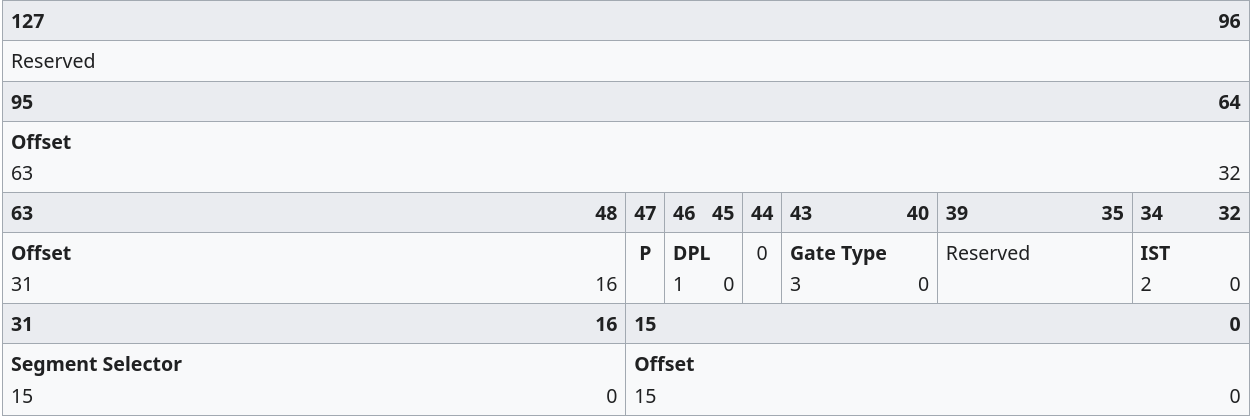
\includegraphics[scale=0.45]{../figures/entrata_idt.png}
\end{center}
come riportato su \url{https://wiki.osdev.org/Interrupt_Descriptor_Table}.

\subsubsection{Gestione dell'interruzione software}
Avevamo visto come il meccanismo dell'interruzione, definito un gate nella IDT, si riduceva al caricamento in RIP dell'indirizzo del gestore e dell'immissione in pila dei seguenti dati:
\begin{table}[H]
	\center
	\begin{tabular} { c | p{5cm} }
		\lstinline|0| & RIP \\
		\lstinline|+1| & CS \\
		\lstinline|+2| & RFLAGS 
	\end{tabular}
\end{table}
Cioè si impostava un nuovo frame sulla pila con i seguenti dati:
\begin{itemize}
	\item L'instruction pointer \textbf{RIP}, da dove si vorrà ripartire nell'esecuzione una volta gestita l'interruzione.
		Notiamo che in verità questo indirizzo, che è fra l'altro in memoria virtuale, è corredato a seconda del tipo di gate dall'\textbf{SS} (\textit{Stack Segment}) o dal \textbf{TSS} (\textit{Task State Segment}), utili alla memoria segmentata che come abbiamo visto non ci è di interesse. La caratteristica importante è che si conserva un riferimento a dove ripartire, in memoria, nell'esecuzione una volta gestita l'interruzione;
	\item Il contenuto attuale di \textbf{CS}, cioè il contesto al momento della chiamata, che chiaramente vorremo ristabilire in seguito;
	\item Come abbiamo visto, anche \textbf{RFLAGS} viene memorizzato, in quanto gli interrupt mascherabili vengono mascherati in fase di gestione di un interrupt sistema (attraverso il flag \textbf{IF}), e vogliamo resettare questo comportamente al termine della gestione.
\end{itemize}

A questo punto l'unica differenza nella chiamata di interrupt in caso di cambio di contesto sta effettivamente nella transizione fra due \textbf{pile}: la separazione fra contesto utente e contesto sistema viene infatti resa possibile anche dalla presenza di due pile separate, di cui l'ultima chiaramente sta in memoria protetta.
Il programma è normalmente in esecuzione nella pila utente: al momento del sollevamento di un interruzione software, si passa all'esecuzione (se alcune condizioni che vedremo fra poco sono rispettate) della routine di gestione definita dal sistema operativo.
Questo richiede un modo per preservare la posizione della pila utente, da cui ci spostiamo quando passiamo alla pila sistema.
Facciamo ciò conservando il vecchio \textbf{RSP}, immettendolo in pila prima dei registri visti prima, cioè creando un frame del tipo:
\begin{table}[H]
	\center
	\begin{tabular} { c | p{7cm} }
		\lstinline|0| & RIP \\
		\lstinline|+1| & CS \\
		\lstinline|+2| & RFLAGS \\ 
		\lstinline|+3| & RSP (Pila utente)
	\end{tabular}
\end{table}
Il vecchio valore di RSP permetterà, fra l'altro, di accedere e modificare il contesto del \textit{processo} in esecuzione con la sua pila utente.

Un caso particolare ma permesso è rappresentato dalla situazione dove \textbf{L}, il livello di destinazione, corrisponde allo stato attuale (ad esempio, sono permesse chiamate di interruzioni da contesto utente a contesto utente, o da contesto sistema a contesto sistema).
In questo caso, chiaramente, tutta questa operazione verrà svolta su un unica pila (sia questa la pila utente o la pila sistema).
Noteremo fra poco come questa possibilità rivela delle falle di sicurezza che vanno gestite.

\subsubsection{Transizione da contesto sistema a contesto utente}
La transizione inversa a quella vista adesso viene fatta semplicemente ritornando dall'interruzione attraverso la \lstinline|IRETQ|.
In questo caso si preleva dalla pila sistema (utente se eravamo in un interruzione a gestione livello utente) le informazioni che vi avevamo inserito al momento della chiamata dell'interruzione (RIP, CS ed EFLAGS) e si ristabilisce lo stato precedente al sollevamento dell'istruzione.
Anche qui vi sono delle particolarità, che verranno spiegato, assieme a quelle annunciate in precedenza, nel paragrafo seguente.

\subsubsection{Particolarità della gestione delle interruzioni software}
Notiamo una particolarità riguardo alla transizione di contesto in fase di chiamata dell'interruzione (nota osservando il contesto attuale e l'L dell'interruzione lanciata), e riguardo alla transizione di contesto in fase di ritorno dall'interruzione (nota osservando il contesto attuale e il contesto salvato in pila).

Infatti, in fase di chiamata (quando si usa la \lstinline|INT|), se L è minore del contesto corrente, viene lanciato un errore.
La motivazione è principalmente una questione di simmetria nel meccanismo di chiamata delle interruzioni, piuttosto che una ragione di sicurezza: si vuole che le interruzioni ci portino in contesti maggiori o uguali del livello presente in CS.

Viceversa, se si prova a passare ad un livello superiore in fase di ritorno dall'interuzione (cioè quando si usa la \lstinline|IRETQ|), viene lanciato un altro errore.
La motivazione è che, visto che prevediamo nell'IDT il flag L, livello di destinazione, che permette di chiamare interruzioni in contesto utente, l'utente potrebbe impostare un frame di pila dove si richiede effettivamente l'accesso ad un livello di protezione superiore, e poi usare \lstinline|IRETQ| per ritornare da tale frame di pila e passare quindi a tale livello di accesso.

\end{document} 


\documentclass[a4paper,11pt]{article}
\usepackage[a4paper, margin=8em]{geometry}

% usa i pacchetti per la scrittura in italiano
\usepackage[french,italian]{babel}
\usepackage[T1]{fontenc}
\usepackage[utf8]{inputenc}
\frenchspacing 

% usa i pacchetti per la formattazione matematica
\usepackage{amsmath, amssymb, amsthm, amsfonts}

% usa altri pacchetti
\usepackage{gensymb}
\usepackage{hyperref}
\usepackage{standalone}

\usepackage{colortbl}

\usepackage{xstring}
\usepackage{karnaugh-map}

% imposta il titolo
\title{Appunti Calcolatori Elettronici}
\author{Luca Seggiani}
\date{2025}

% imposta lo stile
% usa helvetica
\usepackage[scaled]{helvet}
% usa palatino
\usepackage{palatino}
% usa un font monospazio guardabile
\usepackage{lmodern}

\renewcommand{\rmdefault}{ppl}
\renewcommand{\sfdefault}{phv}
\renewcommand{\ttdefault}{lmtt}

% circuiti
\usepackage{circuitikz}
\usetikzlibrary{babel}

% testo cerchiato
\newcommand*\circled[1]{\tikz[baseline=(char.base)]{
            \node[shape=circle,draw,inner sep=2pt] (char) {#1};}}

% disponi il titolo
\makeatletter
\renewcommand{\maketitle} {
	\begin{center} 
		\begin{minipage}[t]{.8\textwidth}
			\textsf{\huge\bfseries \@title} 
		\end{minipage}%
		\begin{minipage}[t]{.2\textwidth}
			\raggedleft \vspace{-1.65em}
			\textsf{\small \@author} \vfill
			\textsf{\small \@date}
		\end{minipage}
		\par
	\end{center}

	\thispagestyle{empty}
	\pagestyle{fancy}
}
\makeatother

% disponi teoremi
\usepackage{tcolorbox}
\newtcolorbox[auto counter, number within=section]{theorem}[2][]{%
	colback=blue!10, 
	colframe=blue!40!black, 
	sharp corners=northwest,
	fonttitle=\sffamily\bfseries, 
	title=Teorema~\thetcbcounter: #2, 
	#1
}

% disponi definizioni
\newtcolorbox[auto counter, number within=section]{definition}[2][]{%
	colback=red!10,
	colframe=red!40!black,
	sharp corners=northwest,
	fonttitle=\sffamily\bfseries,
	title=Definizione~\thetcbcounter: #2,
	#1
}

% disponi codice
\usepackage{listings}
\usepackage[table]{xcolor}

\definecolor{codegreen}{rgb}{0,0.6,0}
\definecolor{codegray}{rgb}{0.5,0.5,0.5}
\definecolor{codepurple}{rgb}{0.58,0,0.82}
\definecolor{backcolour}{rgb}{0.95,0.95,0.92}

\lstdefinestyle{codestyle}{
		backgroundcolor=\color{black!5}, 
		commentstyle=\color{codegreen},
		keywordstyle=\bfseries\color{magenta},
		numberstyle=\sffamily\tiny\color{black!60},
		stringstyle=\color{green!50!black},
		basicstyle=\ttfamily\footnotesize,
		breakatwhitespace=false,         
		breaklines=true,                 
		captionpos=b,                    
		keepspaces=true,                 
		numbers=left,                    
		numbersep=5pt,                  
		showspaces=false,                
		showstringspaces=false,
		showtabs=false,                  
		tabsize=2
}

\lstdefinestyle{shellstyle}{
		backgroundcolor=\color{black!5}, 
		basicstyle=\ttfamily\footnotesize\color{black}, 
		commentstyle=\color{black}, 
		keywordstyle=\color{black},
		numberstyle=\color{black!5},
		stringstyle=\color{black}, 
		showspaces=false,
		showstringspaces=false, 
		showtabs=false, 
		tabsize=2, 
		numbers=none, 
		breaklines=true
}


\lstdefinelanguage{assembler}{ 
  keywords={AAA, AAD, AAM, AAS, ADC, ADCB, ADCW, ADCL, ADD, ADDB, ADDW, ADDL, AND, ANDB, ANDW, ANDL,
        ARPL, BOUND, BSF, BSFL, BSFW, BSR, BSRL, BSRW, BSWAP, BT, BTC, BTCB, BTCW, BTCL, BTR, 
        BTRB, BTRW, BTRL, BTS, BTSB, BTSW, BTSL, CALL, CBW, CDQ, CLC, CLD, CLI, CLTS, CMC, CMP,
        CMPB, CMPW, CMPL, CMPS, CMPSB, CMPSD, CMPSW, CMPXCHG, CMPXCHGB, CMPXCHGW, CMPXCHGL,
        CMPXCHG8B, CPUID, CWDE, DAA, DAS, DEC, DECB, DECW, DECL, DIV, DIVB, DIVW, DIVL, ENTER,
        HLT, IDIV, IDIVB, IDIVW, IDIVL, IMUL, IMULB, IMULW, IMULL, IN, INB, INW, INL, INC, INCB,
        INCW, INCL, INS, INSB, INSD, INSW, INT, INT3, INTO, INVD, INVLPG, IRET, IRETD, JA, JAE,
        JB, JBE, JC, JCXZ, JE, JECXZ, JG, JGE, JL, JLE, JMP, JNA, JNAE, JNB, JNBE, JNC, JNE, JNG,
        JNGE, JNL, JNLE, JNO, JNP, JNS, JNZ, JO, JP, JPE, JPO, JS, JZ, LAHF, LAR, LCALL, LDS,
        LEA, LEAVE, LES, LFS, LGDT, LGS, LIDT, LMSW, LOCK, LODSB, LODSD, LODSW, LOOP, LOOPE,
        LOOPNE, LSL, LSS, LTR, MOV, MOVB, MOVW, MOVL, MOVSB, MOVSD, MOVSW, MOVSX, MOVSXB,
        MOVSXW, MOVSXL, MOVZX, MOVZXB, MOVZXW, MOVZXL, MUL, MULB, MULW, MULL, NEG, NEGB, NEGW,
        NEGL, NOP, NOT, NOTB, NOTW, NOTL, OR, ORB, ORW, ORL, OUT, OUTB, OUTW, OUTL, OUTSB, OUTSD,
        OUTSW, POP, POPL, POPW, POPB, POPA, POPAD, POPF, POPFD, PUSH, PUSHL, PUSHW, PUSHB, PUSHA, 
				PUSHAD, PUSHF, PUSHFD, RCL, RCLB, RCLW, MOVSL, MOVSB, MOVSW, STOSL, STOSB, STOSW, LODSB, LODSW,
				LODSL, INSB, INSW, INSL, OUTSB, OUTSL, OUTSW
        RCLL, RCR, RCRB, RCRW, RCRL, RDMSR, RDPMC, RDTSC, REP, REPE, REPNE, RET, ROL, ROLB, ROLW,
        ROLL, ROR, RORB, RORW, RORL, SAHF, SAL, SALB, SALW, SALL, SAR, SARB, SARW, SARL, SBB,
        SBBB, SBBW, SBBL, SCASB, SCASD, SCASW, SETA, SETAE, SETB, SETBE, SETC, SETE, SETG, SETGE,
        SETL, SETLE, SETNA, SETNAE, SETNB, SETNBE, SETNC, SETNE, SETNG, SETNGE, SETNL, SETNLE,
        SETNO, SETNP, SETNS, SETNZ, SETO, SETP, SETPE, SETPO, SETS, SETZ, SGDT, SHL, SHLB, SHLW,
        SHLL, SHLD, SHR, SHRB, SHRW, SHRL, SHRD, SIDT, SLDT, SMSW, STC, STD, STI, STOSB, STOSD,
        STOSW, STR, SUB, SUBB, SUBW, SUBL, TEST, TESTB, TESTW, TESTL, VERR, VERW, WAIT, WBINVD,
        XADD, XADDB, XADDW, XADDL, XCHG, XCHGB, XCHGW, XCHGL, XLAT, XLATB, XOR, XORB, XORW, XORL},
  keywordstyle=\color{blue}\bfseries,
  ndkeywordstyle=\color{darkgray}\bfseries,
  identifierstyle=\color{black},
  sensitive=false,
  comment=[l]{\#},
  morecomment=[s]{/*}{*/},
  commentstyle=\color{purple}\ttfamily,
  stringstyle=\color{red}\ttfamily,
  morestring=[b]',
  morestring=[b]"
}

\lstset{language=assembler, style=codestyle}

% disponi sezioni
\usepackage{titlesec}

\titleformat{\section}
	{\sffamily\Large\bfseries} 
	{\thesection}{1em}{} 
\titleformat{\subsection}
	{\sffamily\large\bfseries}   
	{\thesubsection}{1em}{} 
\titleformat{\subsubsection}
	{\sffamily\normalsize\bfseries} 
	{\thesubsubsection}{1em}{}

% tikz
\usepackage{tikz}

% float
\usepackage{float}

% grafici
\usepackage{pgfplots}
\pgfplotsset{width=10cm,compat=1.9}

% disponi alberi
\usepackage{forest}

\forestset{
	rectstyle/.style={
		for tree={rectangle,draw,font=\large\sffamily}
	},
	roundstyle/.style={
		for tree={circle,draw,font=\large}
	}
}

% disponi algoritmi
\usepackage{algorithm}
\usepackage{algorithmic}
\makeatletter
\renewcommand{\ALG@name}{Algoritmo}
\makeatother

% disponi numeri di pagina
\usepackage{fancyhdr}
\fancyhf{} 
\fancyfoot[L]{\sffamily{\thepage}}

\makeatletter
\fancyhead[L]{\raisebox{1ex}[0pt][0pt]{\sffamily{\@title \ \@date}}} 
\fancyhead[R]{\raisebox{1ex}[0pt][0pt]{\sffamily{\@author}}}
\makeatother

\begin{document}
% sezione (data)
\section{Lezione del 18-03-25}

% stili pagina
\thispagestyle{empty}
\pagestyle{fancy}

% testo
\subsection{Time-sharing}
Abbiamo accennato al funzionamento dei calcolatori in modalità \textit{batch}, dove più programmi vengono eseguiti in sequenza, uno dopo l'altro.

Un paradigma sicuramente più piacevole per l'utente, e più diffuso al giorno d'oggi, è quello del \textbf{time-sharing}, dove il processore dà l'illusione agli utenti di portare avanti più attività contemporaneamente, mentre il tempo della CPU è in verita diviso in frammenti temporali ridotti dove si dedica a ogni attività singolarmente.

Il meccanismo stesso della protezione che abbiamo introdotto alla lezione precedente serve appunto a difendere i programmi l'uno dall'altro in caso di esecuzione "parallela" (da non confondere col \textit{multithreading}).
Infatti, anche se è un concetto nato nei \textit{mainframe} a uso pubblico, la protezione si è subito diffusa anche nelle macchine personali degli utenti, in modo da difendere non più programmi di diversi utenti ma più programmi dello \textit{stesso} utente, magari soggetti a bug che potrebbero corrompere lo stato di altri programmi o dell'intero sistema.

Oggi il meccanismo di protezione si trova in tutti i calcolatori moderni, dai telefoni cellulari ai supercomputer, ed è risparmiato solo nel caso dei microcontrollori più semplici.

La domanda che ci poniamo adesso è quindi quella di \textit{come} realizzare un sistema capace di dare quest'illusione dell'esecuzione "parallela" di più programmi, che avevamo introdotto all'inizio del corso come \textbf{multiprogrammazione}.

\subsubsection{Processo}
Chiamiamo \textbf{processo} un programma in esecuzione. Ciò che vorremo eseguire in parellelo sono, più propriamente, non programmi ma \textit{processi}.

Intendiamo quindi un processo non come il codice che definisce un programma, ma come il programma stesso una volta che viene messo in esecuzione nel calcolatore, quindi tutti gli stati di elaborazione (disposti nel tempo) del calcolatore nell'esecuzione di tale programma.

Il modo in cui andremo a definire il paradigma della multiprogrammazione è assumendo un processo come un insieme di operazioni \textbf{atomiche}, che possono essere interrotte al loro termine o prima del loro inizio, e che bastano insieme all'istruzione successiva del codice a determinare lo stato successivo di esecuzione del processo.

\subsubsection{Contesto}
Un altro concetto chiave nella multiprogrammazione sarà il \textbf{contesto} di un processo.
Avevamo parlato di contesto in termini di protezine: adesso diamo un significato leggermente diverso.
Ogni processo si aspetterà infatti di trovarsi nel \textit{suo} contesto personale: le operazioni intaccheranno i suoi registri, che si aspetta essere l'unico a modificare, ecc...
Il sistema operativo dovrà quindi essere in grado di fornire a ogni processo il suo contesto specifico.

Vediamo che questa idea si può tradurre già lato software.
Il \textbf{cambio di contesto} può essere infatti effettuato, prendendo l'esempio dei soli registri, mantenendo una struttura data che contiene un'entrata per ogni registro.
Al momento del cambio basterà copiare l'insieme dei registri corrispondenti al contesto di un certo processo nei registri veri e propri del processore.

Un discorso analogo sarà quella della memoria: ogni processo si aspetterà che al suo contesto corrisponda una sua copia della memoria.
Possiamo mantenere un'altra struttura dati, simile a quella posta per i registri, che si occupa di mantenere informazioni riguardo alle regioni di memoria corrispondenti ad ogni contesto, e caricare quindi queste in una sezione dedicata su e della memoria stessa, o per semplicità su e dall'hard disk (così erano i primi sistemi time-sharing).
Vedremo più nel dettaglio questo aspetto quando introdurremo la \textit{memoria virtuale}.

Facciamo un ultima nota sulla \textit{comunicazione} fra processi: nel caso più semplice, ogni processo non è al corrente dell'esistenza degli altri processi, e gestisce la sua \textit{memoria privata}.
Il sistema che studieremo dispone invece anche di una \textit{memoria condivisa}, che permette ai processi di condividere informazioni fra di loro.

\subsubsection{Kernel}
Il programma che si occupa di effettuare queste operazioni di cambio di contesto si chiama \textbf{kernel} o \textit{nucleo}.
E' sempre in esecuzione in modo sistema e gestisce i contesti e le risorse assegnate ad ogni processo.

Immaginiamo quindi il kernel come un intermediario fra \textbf{processi} e \textbf{hardware}.
Notiamo che questo non significa che kernel e processi sono \textit{contemporaneamente} in esecuzione: questo è impossibile, in quanto la CPU è una sola.
Kernel e processi sono infatti in esecuzione singolarmente, l'uno alla volta, e l'unico modo in cui si restituisce il controllo al kernel da un processo è attraverso i 3 tipi di interruzioni:
\begin{itemize}
	\item Interruzioni esterne (dai dispositivi);
	\item Eccezioni (errori e altri malfunzionamenti, non necessariamente dati da errori di programmazione);
	\item Interruzioni interne (sollevate dall'istruzione \lstinline|INT|).
\end{itemize}

\end{document}


\documentclass[a4paper,11pt]{article}
\usepackage[a4paper, margin=8em]{geometry}

% usa i pacchetti per la scrittura in italiano
\usepackage[french,italian]{babel}
\usepackage[T1]{fontenc}
\usepackage[utf8]{inputenc}
\frenchspacing 

% usa i pacchetti per la formattazione matematica
\usepackage{amsmath, amssymb, amsthm, amsfonts}

% usa altri pacchetti
\usepackage{gensymb}
\usepackage{hyperref}
\usepackage{standalone}

\usepackage{colortbl}

\usepackage{xstring}
\usepackage{karnaugh-map}

% imposta il titolo
\title{Appunti Calcolatori Elettronici}
\author{Luca Seggiani}
\date{2025}

% imposta lo stile
% usa helvetica
\usepackage[scaled]{helvet}
% usa palatino
\usepackage{palatino}
% usa un font monospazio guardabile
\usepackage{lmodern}

\renewcommand{\rmdefault}{ppl}
\renewcommand{\sfdefault}{phv}
\renewcommand{\ttdefault}{lmtt}

% circuiti
\usepackage{circuitikz}
\usetikzlibrary{babel}

% testo cerchiato
\newcommand*\circled[1]{\tikz[baseline=(char.base)]{
            \node[shape=circle,draw,inner sep=2pt] (char) {#1};}}

% disponi il titolo
\makeatletter
\renewcommand{\maketitle} {
	\begin{center} 
		\begin{minipage}[t]{.8\textwidth}
			\textsf{\huge\bfseries \@title} 
		\end{minipage}%
		\begin{minipage}[t]{.2\textwidth}
			\raggedleft \vspace{-1.65em}
			\textsf{\small \@author} \vfill
			\textsf{\small \@date}
		\end{minipage}
		\par
	\end{center}

	\thispagestyle{empty}
	\pagestyle{fancy}
}
\makeatother

% disponi teoremi
\usepackage{tcolorbox}
\newtcolorbox[auto counter, number within=section]{theorem}[2][]{%
	colback=blue!10, 
	colframe=blue!40!black, 
	sharp corners=northwest,
	fonttitle=\sffamily\bfseries, 
	title=Teorema~\thetcbcounter: #2, 
	#1
}

% disponi definizioni
\newtcolorbox[auto counter, number within=section]{definition}[2][]{%
	colback=red!10,
	colframe=red!40!black,
	sharp corners=northwest,
	fonttitle=\sffamily\bfseries,
	title=Definizione~\thetcbcounter: #2,
	#1
}

% disponi codice
\usepackage{listings}
\usepackage[table]{xcolor}

\definecolor{codegreen}{rgb}{0,0.6,0}
\definecolor{codegray}{rgb}{0.5,0.5,0.5}
\definecolor{codepurple}{rgb}{0.58,0,0.82}
\definecolor{backcolour}{rgb}{0.95,0.95,0.92}

\lstdefinestyle{codestyle}{
		backgroundcolor=\color{black!5}, 
		commentstyle=\color{codegreen},
		keywordstyle=\bfseries\color{magenta},
		numberstyle=\sffamily\tiny\color{black!60},
		stringstyle=\color{green!50!black},
		basicstyle=\ttfamily\footnotesize,
		breakatwhitespace=false,         
		breaklines=true,                 
		captionpos=b,                    
		keepspaces=true,                 
		numbers=left,                    
		numbersep=5pt,                  
		showspaces=false,                
		showstringspaces=false,
		showtabs=false,                  
		tabsize=2
}

\lstdefinestyle{shellstyle}{
		backgroundcolor=\color{black!5}, 
		basicstyle=\ttfamily\footnotesize\color{black}, 
		commentstyle=\color{black}, 
		keywordstyle=\color{black},
		numberstyle=\color{black!5},
		stringstyle=\color{black}, 
		showspaces=false,
		showstringspaces=false, 
		showtabs=false, 
		tabsize=2, 
		numbers=none, 
		breaklines=true
}


\lstdefinelanguage{assembler}{ 
  keywords={AAA, AAD, AAM, AAS, ADC, ADCB, ADCW, ADCL, ADD, ADDB, ADDW, ADDL, AND, ANDB, ANDW, ANDL,
        ARPL, BOUND, BSF, BSFL, BSFW, BSR, BSRL, BSRW, BSWAP, BT, BTC, BTCB, BTCW, BTCL, BTR, 
        BTRB, BTRW, BTRL, BTS, BTSB, BTSW, BTSL, CALL, CBW, CDQ, CLC, CLD, CLI, CLTS, CMC, CMP,
        CMPB, CMPW, CMPL, CMPS, CMPSB, CMPSD, CMPSW, CMPXCHG, CMPXCHGB, CMPXCHGW, CMPXCHGL,
        CMPXCHG8B, CPUID, CWDE, DAA, DAS, DEC, DECB, DECW, DECL, DIV, DIVB, DIVW, DIVL, ENTER,
        HLT, IDIV, IDIVB, IDIVW, IDIVL, IMUL, IMULB, IMULW, IMULL, IN, INB, INW, INL, INC, INCB,
        INCW, INCL, INS, INSB, INSD, INSW, INT, INT3, INTO, INVD, INVLPG, IRET, IRETD, JA, JAE,
        JB, JBE, JC, JCXZ, JE, JECXZ, JG, JGE, JL, JLE, JMP, JNA, JNAE, JNB, JNBE, JNC, JNE, JNG,
        JNGE, JNL, JNLE, JNO, JNP, JNS, JNZ, JO, JP, JPE, JPO, JS, JZ, LAHF, LAR, LCALL, LDS,
        LEA, LEAVE, LES, LFS, LGDT, LGS, LIDT, LMSW, LOCK, LODSB, LODSD, LODSW, LOOP, LOOPE,
        LOOPNE, LSL, LSS, LTR, MOV, MOVB, MOVW, MOVL, MOVSB, MOVSD, MOVSW, MOVSX, MOVSXB,
        MOVSXW, MOVSXL, MOVZX, MOVZXB, MOVZXW, MOVZXL, MUL, MULB, MULW, MULL, NEG, NEGB, NEGW,
        NEGL, NOP, NOT, NOTB, NOTW, NOTL, OR, ORB, ORW, ORL, OUT, OUTB, OUTW, OUTL, OUTSB, OUTSD,
        OUTSW, POP, POPL, POPW, POPB, POPA, POPAD, POPF, POPFD, PUSH, PUSHL, PUSHW, PUSHB, PUSHA, 
				PUSHAD, PUSHF, PUSHFD, RCL, RCLB, RCLW, MOVSL, MOVSB, MOVSW, STOSL, STOSB, STOSW, LODSB, LODSW,
				LODSL, INSB, INSW, INSL, OUTSB, OUTSL, OUTSW
        RCLL, RCR, RCRB, RCRW, RCRL, RDMSR, RDPMC, RDTSC, REP, REPE, REPNE, RET, ROL, ROLB, ROLW,
        ROLL, ROR, RORB, RORW, RORL, SAHF, SAL, SALB, SALW, SALL, SAR, SARB, SARW, SARL, SBB,
        SBBB, SBBW, SBBL, SCASB, SCASD, SCASW, SETA, SETAE, SETB, SETBE, SETC, SETE, SETG, SETGE,
        SETL, SETLE, SETNA, SETNAE, SETNB, SETNBE, SETNC, SETNE, SETNG, SETNGE, SETNL, SETNLE,
        SETNO, SETNP, SETNS, SETNZ, SETO, SETP, SETPE, SETPO, SETS, SETZ, SGDT, SHL, SHLB, SHLW,
        SHLL, SHLD, SHR, SHRB, SHRW, SHRL, SHRD, SIDT, SLDT, SMSW, STC, STD, STI, STOSB, STOSD,
        STOSW, STR, SUB, SUBB, SUBW, SUBL, TEST, TESTB, TESTW, TESTL, VERR, VERW, WAIT, WBINVD,
        XADD, XADDB, XADDW, XADDL, XCHG, XCHGB, XCHGW, XCHGL, XLAT, XLATB, XOR, XORB, XORW, XORL},
  keywordstyle=\color{blue}\bfseries,
  ndkeywordstyle=\color{darkgray}\bfseries,
  identifierstyle=\color{black},
  sensitive=false,
  comment=[l]{\#},
  morecomment=[s]{/*}{*/},
  commentstyle=\color{purple}\ttfamily,
  stringstyle=\color{red}\ttfamily,
  morestring=[b]',
  morestring=[b]"
}

\lstset{language=assembler, style=codestyle}

% disponi sezioni
\usepackage{titlesec}

\titleformat{\section}
	{\sffamily\Large\bfseries} 
	{\thesection}{1em}{} 
\titleformat{\subsection}
	{\sffamily\large\bfseries}   
	{\thesubsection}{1em}{} 
\titleformat{\subsubsection}
	{\sffamily\normalsize\bfseries} 
	{\thesubsubsection}{1em}{}

% tikz
\usepackage{tikz}

% float
\usepackage{float}

% grafici
\usepackage{pgfplots}
\pgfplotsset{width=10cm,compat=1.9}

% disponi alberi
\usepackage{forest}

\forestset{
	rectstyle/.style={
		for tree={rectangle,draw,font=\large\sffamily}
	},
	roundstyle/.style={
		for tree={circle,draw,font=\large}
	}
}

% disponi algoritmi
\usepackage{algorithm}
\usepackage{algorithmic}
\makeatletter
\renewcommand{\ALG@name}{Algoritmo}
\makeatother

% disponi numeri di pagina
\usepackage{fancyhdr}
\fancyhf{} 
\fancyfoot[L]{\sffamily{\thepage}}

\makeatletter
\fancyhead[L]{\raisebox{1ex}[0pt][0pt]{\sffamily{\@title \ \@date}}} 
\fancyhead[R]{\raisebox{1ex}[0pt][0pt]{\sffamily{\@author}}}
\makeatother

\begin{document}
% sezione (data)
\section{Lezione del 21-03-25}

% stili pagina
\thispagestyle{empty}
\pagestyle{fancy}

% testo
Andiamo a definire più nei dettagli la struttura di un processo e le modalità secondo le quali questi si possono creare e distruggere.

\subsection{Descrittori di processo}
Un processo è descritto fondalmente da un astrazione, detta \textbf{descrittore di processo}, idealmente contenuta in una qualche locazione contigua, assieme ad altri descrittori, in memoria.
\begin{itemize}
	\item Il primo campo del descrittore sarà un \textbf{indice} numerico unico ad ogni processo;
	\item Dovremo poi tenere conto del \textbf{contesto} del processo, inteso come la copia di tutti i registri del processore. 
\end{itemize}

# fai grafico
[ Creazione ] -> [ Pronto ] -> [ Esecuzione ] -> [ Terminato ]
												/\		   | /\								
												|				\/ |
										  	[ Bloccato ]

I descrittori vengono posti in una struttura dati che ne consente \textbf{schedulazione} e \textbf{dispatch}:
\begin{itemize}
	\item \textbf{Schedulazione:} effettivamente la scelta che il kernel fa, assunto il controllo, su qual'è il prossimo processo da portare in esecuzione (passaggio da processo \textbf{pronto} a processo in \textbf{esecuzione});
	\item \textbf{Dispatch:} l'esecuzione effettiva di una serie di operazioni di tale processo. 
\end{itemize}

I processi possono anche \textbf{bloccarsi}, cioè mettersi in attesa di qualche evento. 

Infine, un processo può \textbf{terminare}, cioè sparire dal sistema (lui e il suo descrittore).
Anche in questo caso il processo deve essere attualmente in esecuzione.

Una transizione che non è prevista da tutti i sistemi è quella di \textbf{preemption}, cioè di ritorno allo stato \textbf{pronto} a controllo dello scheduler.
La maggior parte dei sistemi operativi supporta tale funzionalità, il nucleo che vedremo solo parzialmente.

\subsection{Prima vista dell'esecuzione del kernel}
Dopo il boot della macchina, il kernel si impadronisce della macchina e lancia il primo processo (il processo utente).
Da qui in poi il kernel avrà il controllo solo fra un processo e l'altro, in caso di interruzioni (interne, esterne o eccezioni), e potrà restituirlo solo attraverso il ritorno da gestore con \lstinline|IRETQ|.

Come abbiamo visto, ad ogni chiamata di gestore di interruzione lascia RIP, CS, RFLAGS e RSP al tempo di chiamata dell'interruzione (facendo le opportune distinzioni fra \textit{fault} e \textit{trap}) in pila.
A questo punto il gestore fa una copia dei registri generali, e si ha a quel punto una \textit{"foto"} del processore al momento di attraversamento del gate, che rappresenterà quindi il \textit{contesto} del processo stesso al momento della chiamata dell'interruzione.

In questo, sfrutteremo delle routine (\lstinline|salva_stato| e \lstinline|carica_stato|) all'avvio e al termine di ogni gestore, che si occupano di salvare e caricare il contesto del processo attualmente in esecuzione.
Per conoscere quale questo processo sia, si mantiene una variabile globale nel sistema, \lstinline|esecuzione|, che punta al descrittore del processo (che è dove vogliamo mettere il contesto stesso).

I processi pronti staranno in una certa struttura dati, ordinata per la \textbf{priorità} (un altro valore che manteniamo nel descrittore di processo) di ogni processo.
Un gestore di interruzione di base, quindi, si potrebbe magari occupare di passare al contesto e all'esecuzione del processo di priorità più alta a intervalli regolari, magari regolato da un timer (cosiddetto \textit{timeslicing}).

Altre situazioni, più vicine a noi, sono quelle del termine di una gestione di un interruzione esterna, o bloccaggio automatico di un processo, dove il kernel deve selezionare il prossimo processo da eseguire, scegliendo chiaramente quello a priorità più alta.

Inseriamo un processo fittizio, \textit{dummy}, nella lista dei processi pronti con la priorità più bassa possibile.
Questo ci assicurerà di non trovarci mai una situazione dove nessun processo è pronto all'esecuzione, e quindi avere sempre qualcosa a cui il kernel può passare (idealmente il processo dummy effettua solo un ciclo a vuoto).

Un ulteriore dettaglio è quello dello stato del processo alla sua creazione.
Non è infatti realistico pensare di controllare se quel processo richiede inizializzazione ogni volta che si ritorna da un interruzione gestita a livello sistema.
Alla creazione del processo, quindi, vogliamo svolgere le seguenti azioni in modo che il processo venga eseguito per la prima volta già in uno stato completo:
\begin{itemize}
	\item Allocare una \textbf{pila sistema} dedicata al processo;
	\item Inizializzare la pila sistema. Questo consisterà nell'inizializzare a loro volta: 
		\begin{itemize}
			\item IP alla prima istruzione del processo;
			\item CS al segmento livello utente dove si trova il processo;
			\item FLAG a quanto viene richiesto dallo standard C++ al momento di avvio (solitamente tutto a 0), con l'eccezione di IF a 1.
		\end{itemize}
	\item Allocare il \textbf{descrittore} di processo, e mettere quel processo fra i processi pronti;
	\item Inizializzare il descrittore. Questo consiste nell'inizializzare a loro volta:
		\begin{itemize}
			\item Un puntatore alla pila sistema appena definita;
			\item Il contesto del processo;
			\item L'\textbf{argomento} di chiamata del processo;
			\item L'\textbf{IOPL}, \textit{IO Privilege Level}, che specifica la possibilità o meno del processo di accedere all'IO. # approfondisci
		\end{itemize}
\end{itemize}

# domanda: ma esiste una copia dei registri sia in contesto sia nella pila di stack?

\end{document}


\documentclass[a4paper,11pt]{article}
\usepackage[a4paper, margin=8em]{geometry}

% usa i pacchetti per la scrittura in italiano
\usepackage[french,italian]{babel}
\usepackage[T1]{fontenc}
\usepackage[utf8]{inputenc}
\frenchspacing 

% usa i pacchetti per la formattazione matematica
\usepackage{amsmath, amssymb, amsthm, amsfonts}

% usa altri pacchetti
\usepackage{gensymb}
\usepackage{hyperref}
\usepackage{standalone}

\usepackage{colortbl}

\usepackage{xstring}
\usepackage{karnaugh-map}

% imposta il titolo
\title{Appunti Calcolatori Elettronici}
\author{Luca Seggiani}
\date{2025}

% imposta lo stile
% usa helvetica
\usepackage[scaled]{helvet}
% usa palatino
\usepackage{palatino}
% usa un font monospazio guardabile
\usepackage{lmodern}

\renewcommand{\rmdefault}{ppl}
\renewcommand{\sfdefault}{phv}
\renewcommand{\ttdefault}{lmtt}

% circuiti
\usepackage{circuitikz}
\usetikzlibrary{babel}

% testo cerchiato
\newcommand*\circled[1]{\tikz[baseline=(char.base)]{
            \node[shape=circle,draw,inner sep=2pt] (char) {#1};}}

% disponi il titolo
\makeatletter
\renewcommand{\maketitle} {
	\begin{center} 
		\begin{minipage}[t]{.8\textwidth}
			\textsf{\huge\bfseries \@title} 
		\end{minipage}%
		\begin{minipage}[t]{.2\textwidth}
			\raggedleft \vspace{-1.65em}
			\textsf{\small \@author} \vfill
			\textsf{\small \@date}
		\end{minipage}
		\par
	\end{center}

	\thispagestyle{empty}
	\pagestyle{fancy}
}
\makeatother

% disponi teoremi
\usepackage{tcolorbox}
\newtcolorbox[auto counter, number within=section]{theorem}[2][]{%
	colback=blue!10, 
	colframe=blue!40!black, 
	sharp corners=northwest,
	fonttitle=\sffamily\bfseries, 
	title=Teorema~\thetcbcounter: #2, 
	#1
}

% disponi definizioni
\newtcolorbox[auto counter, number within=section]{definition}[2][]{%
	colback=red!10,
	colframe=red!40!black,
	sharp corners=northwest,
	fonttitle=\sffamily\bfseries,
	title=Definizione~\thetcbcounter: #2,
	#1
}

% disponi codice
\usepackage{listings}
\usepackage[table]{xcolor}

\definecolor{codegreen}{rgb}{0,0.6,0}
\definecolor{codegray}{rgb}{0.5,0.5,0.5}
\definecolor{codepurple}{rgb}{0.58,0,0.82}
\definecolor{backcolour}{rgb}{0.95,0.95,0.92}

\lstdefinestyle{codestyle}{
		backgroundcolor=\color{black!5}, 
		commentstyle=\color{codegreen},
		keywordstyle=\bfseries\color{magenta},
		numberstyle=\sffamily\tiny\color{black!60},
		stringstyle=\color{green!50!black},
		basicstyle=\ttfamily\footnotesize,
		breakatwhitespace=false,         
		breaklines=true,                 
		captionpos=b,                    
		keepspaces=true,                 
		numbers=left,                    
		numbersep=5pt,                  
		showspaces=false,                
		showstringspaces=false,
		showtabs=false,                  
		tabsize=2
}

\lstdefinestyle{shellstyle}{
		backgroundcolor=\color{black!5}, 
		basicstyle=\ttfamily\footnotesize\color{black}, 
		commentstyle=\color{black}, 
		keywordstyle=\color{black},
		numberstyle=\color{black!5},
		stringstyle=\color{black}, 
		showspaces=false,
		showstringspaces=false, 
		showtabs=false, 
		tabsize=2, 
		numbers=none, 
		breaklines=true
}


\lstdefinelanguage{assembler}{ 
  keywords={AAA, AAD, AAM, AAS, ADC, ADCB, ADCW, ADCL, ADD, ADDB, ADDW, ADDL, AND, ANDB, ANDW, ANDL,
        ARPL, BOUND, BSF, BSFL, BSFW, BSR, BSRL, BSRW, BSWAP, BT, BTC, BTCB, BTCW, BTCL, BTR, 
        BTRB, BTRW, BTRL, BTS, BTSB, BTSW, BTSL, CALL, CBW, CDQ, CLC, CLD, CLI, CLTS, CMC, CMP,
        CMPB, CMPW, CMPL, CMPS, CMPSB, CMPSD, CMPSW, CMPXCHG, CMPXCHGB, CMPXCHGW, CMPXCHGL,
        CMPXCHG8B, CPUID, CWDE, DAA, DAS, DEC, DECB, DECW, DECL, DIV, DIVB, DIVW, DIVL, ENTER,
        HLT, IDIV, IDIVB, IDIVW, IDIVL, IMUL, IMULB, IMULW, IMULL, IN, INB, INW, INL, INC, INCB,
        INCW, INCL, INS, INSB, INSD, INSW, INT, INT3, INTO, INVD, INVLPG, IRET, IRETD, JA, JAE,
        JB, JBE, JC, JCXZ, JE, JECXZ, JG, JGE, JL, JLE, JMP, JNA, JNAE, JNB, JNBE, JNC, JNE, JNG,
        JNGE, JNL, JNLE, JNO, JNP, JNS, JNZ, JO, JP, JPE, JPO, JS, JZ, LAHF, LAR, LCALL, LDS,
        LEA, LEAVE, LES, LFS, LGDT, LGS, LIDT, LMSW, LOCK, LODSB, LODSD, LODSW, LOOP, LOOPE,
        LOOPNE, LSL, LSS, LTR, MOV, MOVB, MOVW, MOVL, MOVSB, MOVSD, MOVSW, MOVSX, MOVSXB,
        MOVSXW, MOVSXL, MOVZX, MOVZXB, MOVZXW, MOVZXL, MUL, MULB, MULW, MULL, NEG, NEGB, NEGW,
        NEGL, NOP, NOT, NOTB, NOTW, NOTL, OR, ORB, ORW, ORL, OUT, OUTB, OUTW, OUTL, OUTSB, OUTSD,
        OUTSW, POP, POPL, POPW, POPB, POPA, POPAD, POPF, POPFD, PUSH, PUSHL, PUSHW, PUSHB, PUSHA, 
				PUSHAD, PUSHF, PUSHFD, RCL, RCLB, RCLW, MOVSL, MOVSB, MOVSW, STOSL, STOSB, STOSW, LODSB, LODSW,
				LODSL, INSB, INSW, INSL, OUTSB, OUTSL, OUTSW
        RCLL, RCR, RCRB, RCRW, RCRL, RDMSR, RDPMC, RDTSC, REP, REPE, REPNE, RET, ROL, ROLB, ROLW,
        ROLL, ROR, RORB, RORW, RORL, SAHF, SAL, SALB, SALW, SALL, SAR, SARB, SARW, SARL, SBB,
        SBBB, SBBW, SBBL, SCASB, SCASD, SCASW, SETA, SETAE, SETB, SETBE, SETC, SETE, SETG, SETGE,
        SETL, SETLE, SETNA, SETNAE, SETNB, SETNBE, SETNC, SETNE, SETNG, SETNGE, SETNL, SETNLE,
        SETNO, SETNP, SETNS, SETNZ, SETO, SETP, SETPE, SETPO, SETS, SETZ, SGDT, SHL, SHLB, SHLW,
        SHLL, SHLD, SHR, SHRB, SHRW, SHRL, SHRD, SIDT, SLDT, SMSW, STC, STD, STI, STOSB, STOSD,
        STOSW, STR, SUB, SUBB, SUBW, SUBL, TEST, TESTB, TESTW, TESTL, VERR, VERW, WAIT, WBINVD,
        XADD, XADDB, XADDW, XADDL, XCHG, XCHGB, XCHGW, XCHGL, XLAT, XLATB, XOR, XORB, XORW, XORL},
  keywordstyle=\color{blue}\bfseries,
  ndkeywordstyle=\color{darkgray}\bfseries,
  identifierstyle=\color{black},
  sensitive=false,
  comment=[l]{\#},
  morecomment=[s]{/*}{*/},
  commentstyle=\color{purple}\ttfamily,
  stringstyle=\color{red}\ttfamily,
  morestring=[b]',
  morestring=[b]"
}

\lstset{language=assembler, style=codestyle}

% disponi sezioni
\usepackage{titlesec}

\titleformat{\section}
	{\sffamily\Large\bfseries} 
	{\thesection}{1em}{} 
\titleformat{\subsection}
	{\sffamily\large\bfseries}   
	{\thesubsection}{1em}{} 
\titleformat{\subsubsection}
	{\sffamily\normalsize\bfseries} 
	{\thesubsubsection}{1em}{}

% tikz
\usepackage{tikz}

% float
\usepackage{float}

% grafici
\usepackage{pgfplots}
\pgfplotsset{width=10cm,compat=1.9}

% disponi alberi
\usepackage{forest}

\forestset{
	rectstyle/.style={
		for tree={rectangle,draw,font=\large\sffamily}
	},
	roundstyle/.style={
		for tree={circle,draw,font=\large}
	}
}

% disponi algoritmi
\usepackage{algorithm}
\usepackage{algorithmic}
\makeatletter
\renewcommand{\ALG@name}{Algoritmo}
\makeatother

% disponi numeri di pagina
\usepackage{fancyhdr}
\fancyhf{} 
\fancyfoot[L]{\sffamily{\thepage}}

\makeatletter
\fancyhead[L]{\raisebox{1ex}[0pt][0pt]{\sffamily{\@title \ \@date}}} 
\fancyhead[R]{\raisebox{1ex}[0pt][0pt]{\sffamily{\@author}}}
\makeatother

\begin{document}
% sezione (data)
\section{Lezione del 24-03-25}

% stili pagina
\thispagestyle{empty}
\pagestyle{fancy}

% testo
\subsection{Primitive}
Abbiamo introdotto il concetto di primitiva, cioè di routine svolte dal sistema al servizio di un dato programma.
Queste verranno implementate come gestori di interruzioni, quindi non propriamente funzioni, in quanto implicano un passaggio di contesto.
Ciò nonostante, in un linguaggio come il C++ le primitive saranno comunque rappresentate da funzioni, dette \textit{funzioni interfaccia}, scritte in assembly e che hanno il solo compito di usare la funzione \lstinline|INT| con i parametri necessari alla chiamata di una specifica primitiva primitiva.

\subsubsection{Primitiva di creazione di un processo}
Abbiamo visto che la creazione di un processo consiste nell'inizializzazione dalla memoria ad esso dedicata in contesto utente e sistema, alla creazione del suo descrittore e all'inserzione di questo in pila \textit{"pronti"}.
Se la pila è rappresentata come una linked list, l'operazione dovra quindi essere quella di un \textit{inserimento in testa}.

Notiamo che questa operazione non può essere divisa da altre interruzioni, in quanto richiede necessariamente almeno due passaggi, dove fra un passaggio e l'altro la lista viene lasciata in uno stato inconsistente:
\begin{itemize}
	\item Prima si fa puntare il processo al resto della lista;
	\item Poi si fa puntare il puntatore della lista pronti al processo inserito.
\end{itemize}
anche invertendo l'ordine delle operazioni, dopo la prima la lista è inconsistente (in questo caso perché il processo inserito non viene effettivamente visto, nel caso opposto perché non vengono visti tutti gli altri).

Nel caso di routine di sistema basterà abbassare il flag \lstinline|IF|, disabilitando effettivamente le interruzioni, durante tutta la durata della routine.
A questo punto basterà evitare di generare eccezioni, e non usare mai l'istruzione \lstinline|INT|, per ottenere una routine che viene eseguita dal processore nella sua interezza senza il rischio di interruzioni.
Chiamiamo codice di questo tipo \textbf{codice atomico}.
Il kernel Linux, ad esempio, \textit{non} è atomico.

\subsubsection{Disposizione delle primitive}
La memoria del calcolatore conterrà in qualsiasi momento la tabella IDT, di cui abbiamo detto le prime 32 entrate rappresentano le eccezioni.
Siamo quindi liberi di usare i gate dal 33 in poi per implementare le primitive.
Per queste primitive dobbiamo impostare i parametri:
\begin{itemize}
	\item \textbf{P:} 1, per attivare il gate;
	\item \textbf{L:} sistema, in quanto le primitive devono essere svolte a livello sistema;
	\item \textbf{DPL:} utente, in quanto le primitive devono essere accessibili all'utente;
	\item L'indirizzo effettivo della routine, implementata (in assembly, serve \lstinline|IRET|), che deve trovarsi da qualche altra parte;
	\item \textbf{I/T:} tipo interrupt (interruzioni esterne mascherabili disabilitate).
\end{itemize}

Notiamo che l'interruzione esterna non mascherabile 2 è comunque in grado di bloccare le nostre istruzioni atomiche.
Questo non è importante, in quanto abbiamo detto la useremo per casi particolarmente catastrofici (dove magari la salvaguardia dei dati dell'utente e del sistema e di maggiore priorità rispetto allo stato dei processi).

La struttura della routine sarà quindi tipicamente:
\begin{lstlisting}[language=assembler, style=codestyle]	
primitiva:
	CALL salva_stato
	CALL c_primitiva
	CALL carica_stato
	IRETQ
\end{lstlisting}

dove \lstinline|c_primitiva| è una funzione, scritta in C++, che termina con una \lstinline|RET| e lascia quindi che \lstinline|primitiva| restituisca il controllo all'utente con \lstinline|IRETQ|.

Per chiamare la primitiva da C++, come abbiamo detto, ci doteremo di una funzione di interfaccia del tipo:
\begin{lstlisting}[language=assembler, style=codestyle]	
primitiva_i:
	INT $ tipo %il tipo di primitiva 
	RET
\end{lstlisting}

\subsubsection{Passaggio di parametri alla primitiva}
Supponiamo di voler passare dei parametri alla nostra primitiva.
La funzione di interfaccia dovrà semplicemente essere modificata per accettare dati parametri (\lstinline|primitiva_i(params...)|).

A questo punto la \lstinline|primitiva_i| potrà svolgere il passaggio effettivo sfruttando i registri, solitamente il solo registro \lstinline|%EAX| (in quanto \lstinline|salva_stato| non modifica i registri).

\subsubsection{Passaggio di parametri dalla primitiva}
Per avere una restituzione di parametri da parte della primitiva la situazione è più complicata, in quanto abbiamo una chiamata a \lstinline|carica_stato| prima del ritorno della primitiva per \lstinline|IRETQ|.

Abbiamo però accesso al contesto di processo, nel descrittore di processo, e possiamo quindi modificare i registri che ci interessano direttamente lì.

\subsubsection{Implementazione delle primitive processo}
Vediamo quindi l'implementazione effettiva delle primitive relative a creazione e terminazione dei processi, cioè le \lstinline|activate_p| e \lstinline|terminate_p|.
Queste chiaramente vengono chiamate da un handler scritto in assembly, che si occupa di salvare e caricare il contesto correttamente, in modo da non intaccare i registri in uso dal processo in \lstinline|esecuzione|.

\begin{itemize}
	\item \lstinline|activate_p|: questa sfrutta una funzione, \lstinline|crea_processo| (per adesso non significativa), che si occupa di creare effettivamente il descrittore di processo.
		Il suo compito è quindi solo quello di controllare che i parametri siano validi, chiamare \lstinline|crea_processo()|, inserire il descrittore in lista pronti e restituire l'id del processo creato.
\begin{lstlisting}[language=C++, style=codestyle]	
// crea un nuovo processo
extern "C" void c_activate_p(void f(natq), natq a, natl prio, natl liv)
{
	des_proc* p; // descrittore per il nuovo processo
	natl id = 0xFFFFFFFF; // id da restituire in caso di fallimento

	// seguono controlli di sicurezza sul livello
	[...]

	// crea effettivamente il descrittore di processo
	p = crea_processo(f, a, prio, liv);

	if (p != nullptr) {
		inserimento_lista(pronti, p);
		processi++;
		id = p->id;			// id del processo creato
						        // (allocato da crea_processo)
	}

	esecuzione->contesto[I_RAX] = id; // restituisci l'id del processo
}
\end{lstlisting}
\item \lstinline|terminate_p|: questa viene chiamata direttamente dal processo in \lstinline|esecuzione|, quando questo desidera essere terminato. 
	In questo, sfrutta una funzione, \lstinline|distruggi_processo()| (anche questa al momento non significativa), che si occupa di ripulire il descrittore del processo (e quindi la sua pila, ecc...).
\begin{lstlisting}[language=C++, style=codestyle]	
// termina il processo attuale 
extern "C" void c_terminate_p()
{
	des_proc* p = esecuzione;

	distruggi_processo(p);
	processi--;
	schedulatore();
}
\end{lstlisting}
\end{itemize}

\subsection{Semafori}
Per gestire l'accesso condiviso ad una risorsa, nel nostro kernel adotteremo il meccanismo dei \textbf{semafori}.

Introdotti da Dijsktra nel 1962, questi si possono meglio modellizzare come una scatola piena di gettoni: ogni utente può mettere un gettone o prelevare un gettone dalla scatola, con la condizione che questa operazione sia atomica: se si tenta di prendere un gettone che non esiste, si resta in attesa finché quel gettone non viene effettivamente immesso nella scatola.

I problemi che vogliamo risolvere sfruttando i semafori sono effettivamente die due categorie:
\begin{itemize}
	\item Problemi di \textbf{mutua esclusione:} assicurarsi che solo un processo possa accedere ad una risorsa in un dato momento.

		In questo caso si associa un gettone alla risorsa: accedere alle risorsa significa prendere il gettone, restituire la risorsa significa reinserire il gettone. L'esistenza di un singolo gettone assicura che solo un processo abbia accesso alla risorsa in un dato momento.
		Al momento della reimmissione del gettone, il processo che ne vince l'accesso sarà nel nostro kernel quello a priorità più alta.

		Notiamo inoltre che un processo che cerca di estrarre un gettone da una scatola vuota (tenta l'accesso ad una risorsa occupata o comunque non disponible) dovrà aspettare che questa risorsa si renda disponibile: rappresenterà quindi il caso perfetto di \textbf{blocco} del processo, che può essere realizzato con \textbf{preemption} nei sistemi che la supportoìano;

	\item Problemi di \textbf{sincronizzazione:} esistono più attività, e ci interessa che alcune attività vengano fatte prime di altre (ordinamento \textit{parziale}).

		Prendiamo l'esempio di avere due processi, A e B, e di volerci assicurare che $\text{A} \rightarrow \text{B}$.
		In questo caso creiamo un semaforo associato al processo A, che parte vuoto. A mette il suo gettone nel semaforo quando finisce la sua esecuzione.
		A questo punto, B preleva il gettone ed esegue.
		Se B avesse provato ad entrare in esecuzione prima che A avesse terminato, non sarebbe riuscito a prelevare il gettone e avrebbe fallito.

		Nel caso di 2 processi (sempre A e B, con A che scrive e B che legge) che devono scambiare dati fra di loro ciclicamente, potremmo usare 2 semafori per realizzare un \textit{handshake}.
		Ad esempio, definiamo quelle che effettivamente sono due variabili logiche sfruttando i semafori, che intendiamo come "buffer scritto" e "buffer letto".
		Il processo A dovrà semplicemente attivare il semaforo "buffer scritto" in fase di scrittura, e il processo B attivare il semaforo "buffer letto" in fase di lettura.
		Abbassando questi semafori al termine delle rispettive operazioni, e assicurandosi, osservando l'altro semaforo, di poter effettivamente procedere ad una nuova operazione, potremmo realizzare il paradigma desiderato. 
\end{itemize}

Dal punto di vista di implementazione, il kernel fornisce una primitiva \lstinline|sem_ini(int val)| che inizializza un semaforo con \lstinline|val| gettoni iniziali, restituendone l'indirizzo.
Da qui in poi i processi hanno accesso alle primitive \lstinline|sem_wait()| e \lstinline|sem_signal()|, che si occupano rispettivamente di richiedere e restiture un gettone.

\subsubsection{Implementazione delle primitive semaforiche}
Vediamo quindi l'implementazione delle primitive relative ai semafori, \lstinline|sem_ini()| \lstinline|sem_wait()| e \lstinline|sem_signal()|.

Innanzitutto, un semaforo viene descritto dalla struttura:
\begin{lstlisting}[language=C++, style=codestyle]	
// descrittore di semaforo
struct des_sem {
	// se >= 0, numero di gettoni contenuti;
	// se < 0, il valore assoluto e' il numero di processi in coda
	int counter;
	// coda di processi bloccati sul semaforo
	des_proc* pointer;
};
\end{lstlisting}

Si definisce quindi, sulla base di un paramero \lstinline|MAX_SEM| che definisce il numero massimo di semaforo in ogni contesto:
\begin{lstlisting}[language=C++, style=codestyle]	
des_sem array_dess[MAX_SEM * 2];
\end{lstlisting}

Il \lstinline|* 2| è motivato dal fatto che si forniscono due array separate di semafori, una al contesto utente e una al contesto sistema.

L'array dei semafori non viene mai ripulita, e i semafori correntemente attivi vengono mantenuti invece da due indici:
\begin{lstlisting}[language=C++, style=codestyle]	
// numero di semafori allocati per il livello utente
natl sem_allocati_utente  = 0;

// numero di semafori allocati per il livello sistema (moduli sistema e I/O)
natl sem_allocati_sistema = 0;
\end{lstlisting}

Le primitive vere e proprie sono quindi:
\begin{itemize}
	\item \lstinline|sem_ini()|: questa si serve di una funzione, \lstinline|alloca_sem()|, che svolge gli opportuni controlli e incrementa l'indice nel vettore dei semafori corretto:
\begin{lstlisting}[language=C++, style=codestyle]
// alloca un semaforo
natl alloca_sem()
{
	// i semafori non vengono mai deallocati, quindi e' possibile allocarli
	// sequenzialmente. Per far questo e' sufficiente ricordare quanti ne
	// abbiamo gia' allocati (variabili sem_allocati_utente e
	// sem_allocati_sistema)

	int liv = liv_chiamante();
	natl i;
	if (liv == LIV_UTENTE) { // semaforo utente
		if (sem_allocati_utente >= MAX_SEM)
			return 0xFFFFFFFF;
		i = sem_allocati_utente;
		sem_allocati_utente++;
	} else { // semaforo sistema
		if (sem_allocati_sistema >= MAX_SEM)
			return 0xFFFFFFFF;
		i = sem_allocati_sistema + MAX_SEM;
		sem_allocati_sistema++;
	}
	return i;
}

// inizializza un semaforo
extern "C" void c_sem_ini(int val)
{
	natl i = alloca_sem();

	if (i != 0xFFFFFFFF)
		array_dess[i].counter = val;

	esecuzione->contesto[I_RAX] = i;
}
\end{lstlisting}
	\item \lstinline|sem_wait()|: è semplicemente:
\begin{lstlisting}[language=C++, style=codestyle]	
extern "C" void c_sem_wait(natl sem)
{
	// controlli sulla validita' del semaforo
	[...]

	des_sem* s = &array_dess[sem];
	s->counter--;

	if (s->counter < 0) {
		inserimento_lista(s->pointer, esecuzione);
		schedulatore();
	}
}
\end{lstlisting}
	\item \lstinline|sem_signal()|: una particolarità di questa è l'uso della funzione \lstinline|inspronti()|, che si rende necessario, come avevamo detto, per non svantaggiare inutilmente il processo corrente alla chiamata di \lstinline|schedulatore()|:
\begin{lstlisting}[language=C++, style=codestyle]	
extern "C" void c_sem_signal(natl sem)
{
	// controlli sulla validita' del semaforo
	[...]

	des_sem* s = &array_dess[sem];
	s->counter++;

	if (s->counter <= 0) {
		des_proc* lavoro = rimozione_lista(s->pointer);
		inspronti();	// preemption
		inserimento_lista(pronti, lavoro);
		schedulatore();	// preemption
	}
}
\end{lstlisting}
\end{itemize}

\end{document}


\documentclass[a4paper,11pt]{article}
\usepackage[a4paper, margin=8em]{geometry}

% usa i pacchetti per la scrittura in italiano
\usepackage[french,italian]{babel}
\usepackage[T1]{fontenc}
\usepackage[utf8]{inputenc}
\frenchspacing 

% usa i pacchetti per la formattazione matematica
\usepackage{amsmath, amssymb, amsthm, amsfonts}

% usa altri pacchetti
\usepackage{gensymb}
\usepackage{hyperref}
\usepackage{standalone}

\usepackage{colortbl}

\usepackage{xstring}
\usepackage{karnaugh-map}

% imposta il titolo
\title{Appunti Calcolatori Elettronici}
\author{Luca Seggiani}
\date{2025}

% imposta lo stile
% usa helvetica
\usepackage[scaled]{helvet}
% usa palatino
\usepackage{palatino}
% usa un font monospazio guardabile
\usepackage{lmodern}

\renewcommand{\rmdefault}{ppl}
\renewcommand{\sfdefault}{phv}
\renewcommand{\ttdefault}{lmtt}

% circuiti
\usepackage{circuitikz}
\usetikzlibrary{babel}

% testo cerchiato
\newcommand*\circled[1]{\tikz[baseline=(char.base)]{
            \node[shape=circle,draw,inner sep=2pt] (char) {#1};}}

% disponi il titolo
\makeatletter
\renewcommand{\maketitle} {
	\begin{center} 
		\begin{minipage}[t]{.8\textwidth}
			\textsf{\huge\bfseries \@title} 
		\end{minipage}%
		\begin{minipage}[t]{.2\textwidth}
			\raggedleft \vspace{-1.65em}
			\textsf{\small \@author} \vfill
			\textsf{\small \@date}
		\end{minipage}
		\par
	\end{center}

	\thispagestyle{empty}
	\pagestyle{fancy}
}
\makeatother

% disponi teoremi
\usepackage{tcolorbox}
\newtcolorbox[auto counter, number within=section]{theorem}[2][]{%
	colback=blue!10, 
	colframe=blue!40!black, 
	sharp corners=northwest,
	fonttitle=\sffamily\bfseries, 
	title=Teorema~\thetcbcounter: #2, 
	#1
}

% disponi definizioni
\newtcolorbox[auto counter, number within=section]{definition}[2][]{%
	colback=red!10,
	colframe=red!40!black,
	sharp corners=northwest,
	fonttitle=\sffamily\bfseries,
	title=Definizione~\thetcbcounter: #2,
	#1
}

% disponi codice
\usepackage{listings}
\usepackage[table]{xcolor}

\definecolor{codegreen}{rgb}{0,0.6,0}
\definecolor{codegray}{rgb}{0.5,0.5,0.5}
\definecolor{codepurple}{rgb}{0.58,0,0.82}
\definecolor{backcolour}{rgb}{0.95,0.95,0.92}

\lstdefinestyle{codestyle}{
		backgroundcolor=\color{black!5}, 
		commentstyle=\color{codegreen},
		keywordstyle=\bfseries\color{magenta},
		numberstyle=\sffamily\tiny\color{black!60},
		stringstyle=\color{green!50!black},
		basicstyle=\ttfamily\footnotesize,
		breakatwhitespace=false,         
		breaklines=true,                 
		captionpos=b,                    
		keepspaces=true,                 
		numbers=left,                    
		numbersep=5pt,                  
		showspaces=false,                
		showstringspaces=false,
		showtabs=false,                  
		tabsize=2
}

\lstdefinestyle{shellstyle}{
		backgroundcolor=\color{black!5}, 
		basicstyle=\ttfamily\footnotesize\color{black}, 
		commentstyle=\color{black}, 
		keywordstyle=\color{black},
		numberstyle=\color{black!5},
		stringstyle=\color{black}, 
		showspaces=false,
		showstringspaces=false, 
		showtabs=false, 
		tabsize=2, 
		numbers=none, 
		breaklines=true
}


\lstdefinelanguage{assembler}{ 
  keywords={AAA, AAD, AAM, AAS, ADC, ADCB, ADCW, ADCL, ADD, ADDB, ADDW, ADDL, AND, ANDB, ANDW, ANDL,
        ARPL, BOUND, BSF, BSFL, BSFW, BSR, BSRL, BSRW, BSWAP, BT, BTC, BTCB, BTCW, BTCL, BTR, 
        BTRB, BTRW, BTRL, BTS, BTSB, BTSW, BTSL, CALL, CBW, CDQ, CLC, CLD, CLI, CLTS, CMC, CMP,
        CMPB, CMPW, CMPL, CMPS, CMPSB, CMPSD, CMPSW, CMPXCHG, CMPXCHGB, CMPXCHGW, CMPXCHGL,
        CMPXCHG8B, CPUID, CWDE, DAA, DAS, DEC, DECB, DECW, DECL, DIV, DIVB, DIVW, DIVL, ENTER,
        HLT, IDIV, IDIVB, IDIVW, IDIVL, IMUL, IMULB, IMULW, IMULL, IN, INB, INW, INL, INC, INCB,
        INCW, INCL, INS, INSB, INSD, INSW, INT, INT3, INTO, INVD, INVLPG, IRET, IRETD, JA, JAE,
        JB, JBE, JC, JCXZ, JE, JECXZ, JG, JGE, JL, JLE, JMP, JNA, JNAE, JNB, JNBE, JNC, JNE, JNG,
        JNGE, JNL, JNLE, JNO, JNP, JNS, JNZ, JO, JP, JPE, JPO, JS, JZ, LAHF, LAR, LCALL, LDS,
        LEA, LEAVE, LES, LFS, LGDT, LGS, LIDT, LMSW, LOCK, LODSB, LODSD, LODSW, LOOP, LOOPE,
        LOOPNE, LSL, LSS, LTR, MOV, MOVB, MOVW, MOVL, MOVSB, MOVSD, MOVSW, MOVSX, MOVSXB,
        MOVSXW, MOVSXL, MOVZX, MOVZXB, MOVZXW, MOVZXL, MUL, MULB, MULW, MULL, NEG, NEGB, NEGW,
        NEGL, NOP, NOT, NOTB, NOTW, NOTL, OR, ORB, ORW, ORL, OUT, OUTB, OUTW, OUTL, OUTSB, OUTSD,
        OUTSW, POP, POPL, POPW, POPB, POPA, POPAD, POPF, POPFD, PUSH, PUSHL, PUSHW, PUSHB, PUSHA, 
				PUSHAD, PUSHF, PUSHFD, RCL, RCLB, RCLW, MOVSL, MOVSB, MOVSW, STOSL, STOSB, STOSW, LODSB, LODSW,
				LODSL, INSB, INSW, INSL, OUTSB, OUTSL, OUTSW
        RCLL, RCR, RCRB, RCRW, RCRL, RDMSR, RDPMC, RDTSC, REP, REPE, REPNE, RET, ROL, ROLB, ROLW,
        ROLL, ROR, RORB, RORW, RORL, SAHF, SAL, SALB, SALW, SALL, SAR, SARB, SARW, SARL, SBB,
        SBBB, SBBW, SBBL, SCASB, SCASD, SCASW, SETA, SETAE, SETB, SETBE, SETC, SETE, SETG, SETGE,
        SETL, SETLE, SETNA, SETNAE, SETNB, SETNBE, SETNC, SETNE, SETNG, SETNGE, SETNL, SETNLE,
        SETNO, SETNP, SETNS, SETNZ, SETO, SETP, SETPE, SETPO, SETS, SETZ, SGDT, SHL, SHLB, SHLW,
        SHLL, SHLD, SHR, SHRB, SHRW, SHRL, SHRD, SIDT, SLDT, SMSW, STC, STD, STI, STOSB, STOSD,
        STOSW, STR, SUB, SUBB, SUBW, SUBL, TEST, TESTB, TESTW, TESTL, VERR, VERW, WAIT, WBINVD,
        XADD, XADDB, XADDW, XADDL, XCHG, XCHGB, XCHGW, XCHGL, XLAT, XLATB, XOR, XORB, XORW, XORL},
  keywordstyle=\color{blue}\bfseries,
  ndkeywordstyle=\color{darkgray}\bfseries,
  identifierstyle=\color{black},
  sensitive=false,
  comment=[l]{\#},
  morecomment=[s]{/*}{*/},
  commentstyle=\color{purple}\ttfamily,
  stringstyle=\color{red}\ttfamily,
  morestring=[b]',
  morestring=[b]"
}

\lstset{language=assembler, style=codestyle}

% disponi sezioni
\usepackage{titlesec}

\titleformat{\section}
	{\sffamily\Large\bfseries} 
	{\thesection}{1em}{} 
\titleformat{\subsection}
	{\sffamily\large\bfseries}   
	{\thesubsection}{1em}{} 
\titleformat{\subsubsection}
	{\sffamily\normalsize\bfseries} 
	{\thesubsubsection}{1em}{}

% tikz
\usepackage{tikz}

% float
\usepackage{float}

% grafici
\usepackage{pgfplots}
\pgfplotsset{width=10cm,compat=1.9}

% disponi alberi
\usepackage{forest}

\forestset{
	rectstyle/.style={
		for tree={rectangle,draw,font=\large\sffamily}
	},
	roundstyle/.style={
		for tree={circle,draw,font=\large}
	}
}

% disponi algoritmi
\usepackage{algorithm}
\usepackage{algorithmic}
\makeatletter
\renewcommand{\ALG@name}{Algoritmo}
\makeatother

% disponi numeri di pagina
\usepackage{fancyhdr}
\fancyhf{} 
\fancyfoot[L]{\sffamily{\thepage}}

\makeatletter
\fancyhead[L]{\raisebox{1ex}[0pt][0pt]{\sffamily{\@title \ \@date}}} 
\fancyhead[R]{\raisebox{1ex}[0pt][0pt]{\sffamily{\@author}}}
\makeatother

\begin{document}
% sezione (data)
\section{Lezione del 25-03-25}

% stili pagina
\thispagestyle{empty}
\pagestyle{fancy}

% testo
\subsection{Attesa}
Esiste un altra primitiva, la \lstinline|delay|, che viene usata per sospendere un processo per un certo istante temporale.

Il kernel sfrutta di per sé il timer 1 per generare interruzioni periodiche, che lo assistano anche solamente a tenere traccia del tempo trascorso durante l'esecuzione.
A questo punto la \lstinline|delay(natl n)| si limita ad aspettare \lstinline|n| clicli del timer.
Un'implementazione naive del timer è quindi quella di una lista di strutture, che rappresentano \textbf{richieste}, che tengono conto del loro conteggio attuale e del processo che le ha invocate.
Un processo crea una richiesta sfruttando la primitiva \lstinline|delay|, che risulta nella creazione di una richiesta e dello spostamento del processo nella lista bloccati.
Il kernel dovrà quindi limitarsi ad aggiornare ad ogni ciclo di timer le richieste, decrementandole, e quindi ad riportare il processo in esecuzione una volta che il conteggio raggiunge 0.

Un modo più efficiente di fare la stessa cosa è quello di memorizzare non il conteggio di ogni richiesta, ma il conteggio \textit{successivo} alla richiesta precedente nella lista d'attesa.
Questo, chiaramente, implicherà un possibile riordinamento della lista in fase di inserzione (chi arriva prima sta in testa).
In questo caso basterà decrementare solo il primo elemento della lista, e in occasione di raggiungimento di 0 eliminare quel processo e i successivi con conteggio aggiuntivo pari a 0.

\subsection{Memoria dinamica}
\lstset{language=C++}
Vediamo alla gestione della memoria dinamica, in particolare alla parola chiave \lstinline|new| fornita dal linguaggio.
Per noi le \lstinline|new| non si tradurranno in altro che chiamate di funzione, che cercano una zona di memoria libera dove allocare il dato desiderato.
Di contro, la \lstinline|delete| si occuperà di deallocare lo stesso dato.

Una domanda che potremmo porci è dove si trova questa memoria.
Per quanto riguarda il \textbf{sistema}, una porzione dedicata viene inizializzta all'avvio e resta tale durante l'esecuzione dello stesso.
Per quanto riguarda l'\textbf{utente}, invece, si dedica un altra porzione di memoria, condivisa fra i processi.
Questa condivisione implica che più processi non possono fornire le loro versioni della funzione \lstinline|new| e \lstinline|delete|, in quanto se queste venissero interrotte (le funzioni utente non sono mai atomiche), lascerebbero la memoria dinamica in uno stato inconsistente per altri processi intenzionati a modificarla.

Si usa quindi un semaforo che tiene conto di chi sta scrivendo in memoria.

\subsection{Memoria virtuale}
Veniamo quindi all'ultimo argomento chiave del corso.
Abbiamo detto che la memoria di sistema è divisa fra sistema e utente.
In ogni momento ci aspettiamo che la memoria utente occupata da due porzioni: una \textbf{parte pubblica}, che rappresenta l'heap condiviso fra processi, e  la \textbf{parte privata}, che rappresenta la memoria relativa ad un \textit{singolo} processo, quello attualmente in esecuzione.
La memoria privata degli altri processi è stata quindi intesa finora come memorizzata separatamente, magari nel disco rigido, con conseguente scaricamento del processo corrente e caricamento del successivo in memoria in fase di cambio di contesto fra processi.

Per i nostri scopi, possiamo assumere anche l'heap come parte della memoria privata. Il problema principale sarà infatti quello di poter memorizzare le immagini della memoria di \textit{più} processi contemporaneamente.
Infatti, storicamente, per \textit{sistema multiprogrammato} si intendeva proprio il sistema in grado di mantenere più processi \textit{in memoria} (il sistema visto finora sarebbe stato detto \textit{multiprocesso}).

Decidiamo quindi di dividere la porzione di memoria utente in più sezioni, associate ad ogni processo.
Potremmo intanto chiederci qual'è la memoria da dedicare ad ogni processo.
La porzione dati e il codice di un programma sono infatti fissi in dimensioni, mentre pila e heap non lo sono.
Storicamente, la memoria richiesta veniva specificata dal programmatore in fase di scrittura del programma.
Quali metodologie si usino oggi non ci è immediatamente di interesse.

Si crea quindi per ogni processo una struttura di questo tipo:
\begin{table}[H]
	\center 
	\begin{tabular} { | c | }
		\sffamily Code \\ 
		\hline
		\sffamily Data \\
		\hline
		\sffamily Heap \\ 
		$\downarrow$ \\
		$\uparrow$ \\
		\sffamily Stack
	\end{tabular}
\end{table}
Dove lo stack e l'heap si espandono in una sola regione, da parti opposte.

\end{document}

\end{document}